
\section{The Graph Neural Network family of Tagger}\label{chap:GN}
As previously advertised in the PFlow- and \gls{vr}-trained \gls{dl1d}, the new generation of classifiers developped for flavour tagging at ATLAS introduce a fundamental shift in design. It moves away from the hieararchical approach, using low-level specialised methods based on physics-inspired algorithm or neural network as input to a high-level neural network. Instead, a single large neural network operates on a rich set of track information as well as some jet features to directly output the per-flavour probabilities. As suggested in Figure \ref{fig:ftagArchi}, this change to the flavour tagging software stacks greatly simplifies the maintenance and development effort, as all attention can be focused on a single network. A new framework called \uppercase{Salt} \cite{SaltCite} built on PyTorch \cite{pytorch} is introduced to simplify the definition and training of multitask multimodal models with multiple \gls{gpu}. This large network is built on a far more powerful and rich architecture with advanced expressive powers, thanks to a modified graph attention network (\gls{gat}) \cite{velickovic2018graph, brody2022how} for \gls{gn1} or a transformer encoder for \gls{gn2} \cite{NIPS_transformerPaper}. 

\begin{figure}[h!]
  \center
  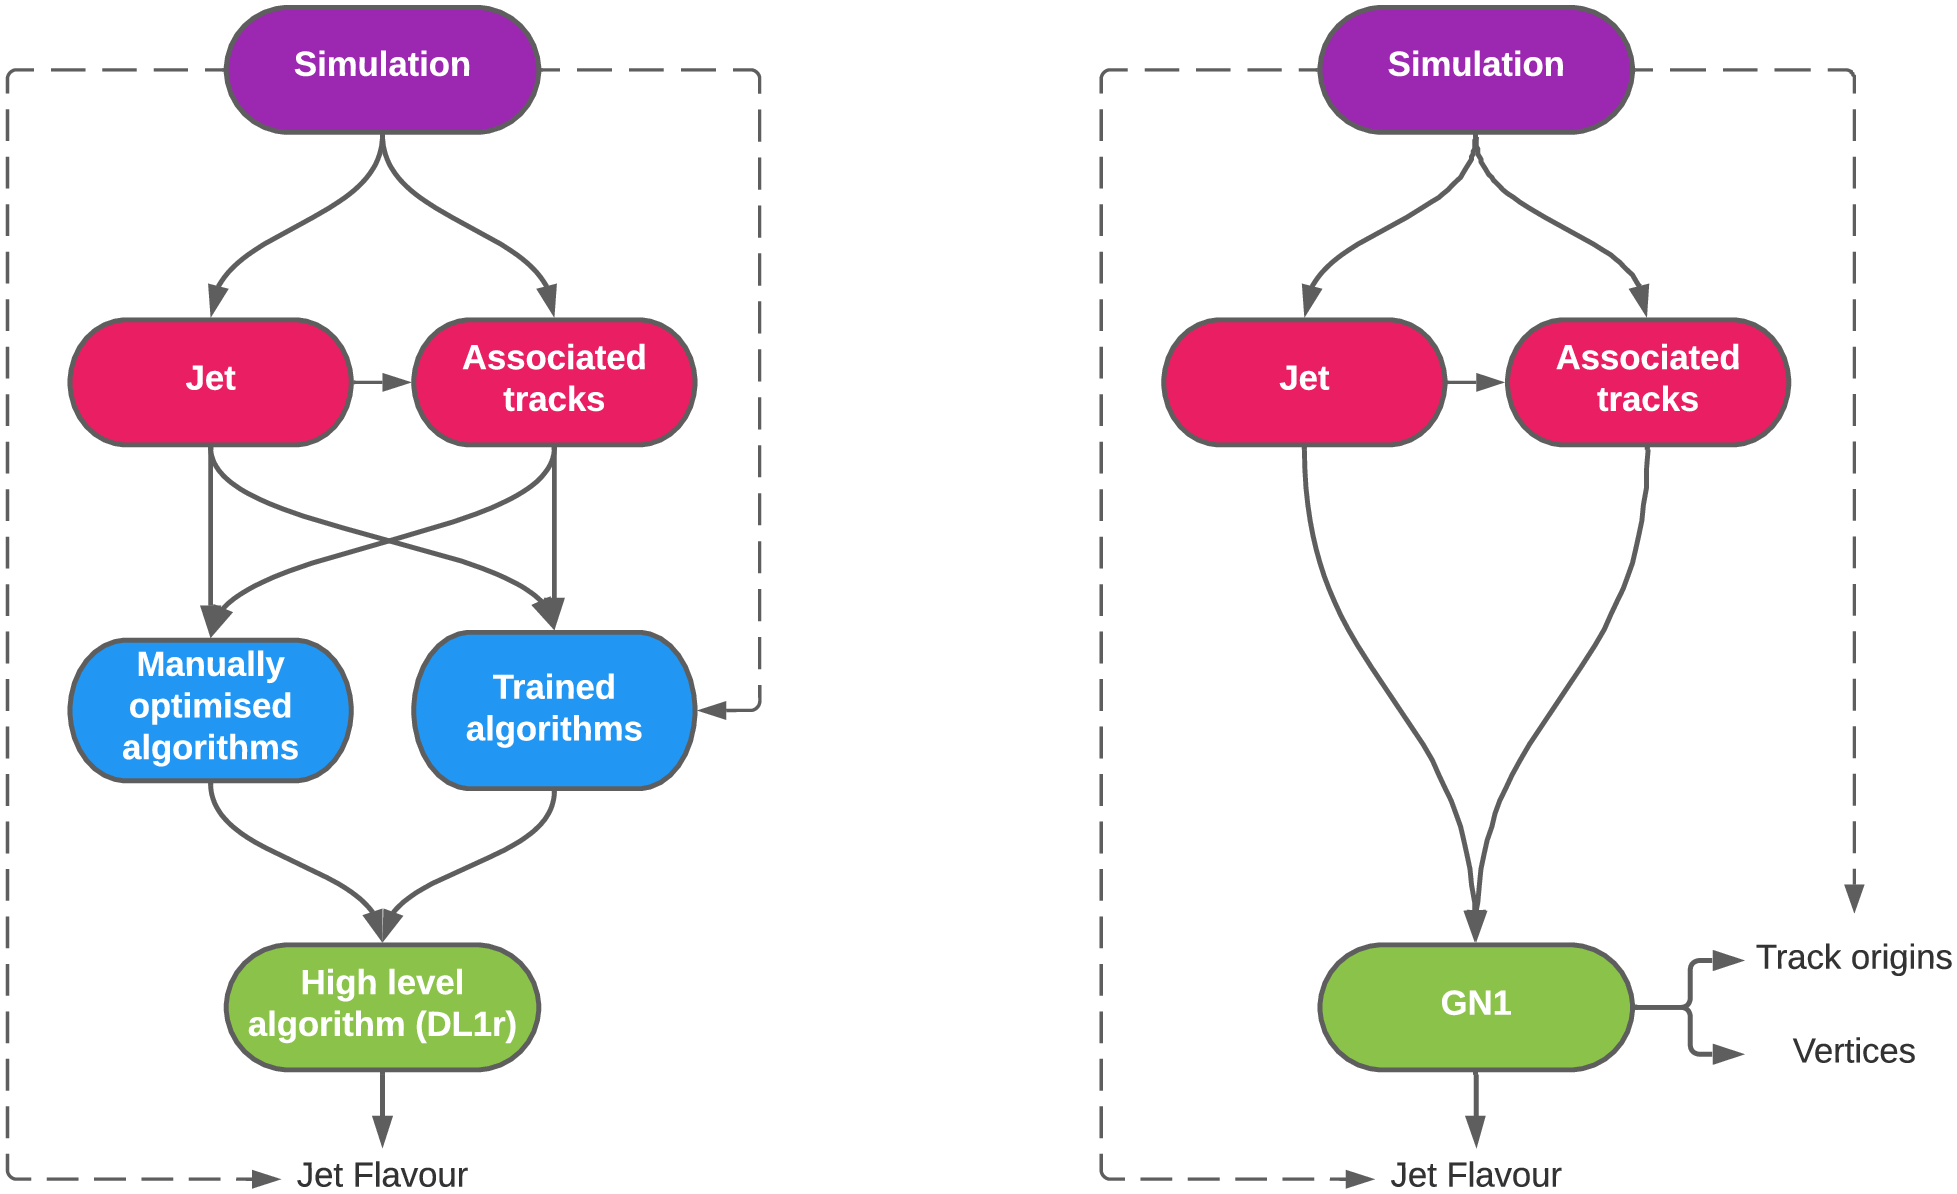
\includegraphics[width=0.9\textwidth]{Images/FTAG/GN/Intro/schematics_difference.png}
  \caption{Comparison of the tagging scheme between the DL1 family (left) and the GN family (right), from \cite{ATL-PHYS-PUB-2022-027}. Solid lines represent reconstructed information while dashed lines represent truth information only accessible from the simulations.} 
  \label{fig:ftagArchi}
\end{figure}

\gls{gn1} uses the information associated with charged tracks in a jet to directly output the flavour-tag probabilities, which are then combined into analogous discriminants to Equations \ref{bdisc} and \ref{cdisc}. This constitutes the primary goal of the network and the real point of developping this network. Alongside predicting the flavour of the jet flavour, auxiliary objectives can also be optimised to aid and guide the training. This so-called \textit{multitask} framework is a common way to input expert knowledge in the design of a \gls{ml} method, focusing the attention of the network on spelled out metrics. In this case, two side tasks are passed along due to the physically meaning they highlight:
\begin{enumerate}
\item Track origin prediction: a classification task aiming to assign a physical process from which the track arises as described in Table \ref{tab:gnTrackOrigin}. The flavour of a jet is strongly correlated to the origin of the tracks. This task brings the attention of the network to this important element as a form of supervised attention \cite{hwang2021selfsupervised}.
\item Vertex prediction: a classification task predicting whether two tracks come from the same vertex. The decays of $b$- and $c$-hadrons include secondary and tertiary vertices inside a jet. Highlighting the compatibility of two tracks to share  a vertex allows the model to infer the presence of such vertices. On the truth side, vertices with a distance < 0.1 mm are merged, and tracks labelled as Pileup or Fake are forced not have any shared vertex.
\end{enumerate}
These complementary objectives use truth information from the simulation and cannot therefore be predicted at inference time on real data. They improve performance during the training by providing useful information on the content of the jets.  A modified approach, pre-training on the auxiliary objectives and then fine-tuning on the primary objective, was not observed to lead to a gain in performance. \\

\begin{table}[h]
  \begin{center}
      \begin{tabular}{cc} 
      	 \hline \hline
          Truth Origin & Description \\ \hline
          Pileup           & From a $pp$ collision other than the primary interaction   \\
          Fake             & Created from the hits of multiple particles  \\
          Primary          & Does not originate from any secondary decay  \\
          fromB            & From the decay of a $b$-hadron  \\
          fromBC           & From a $c$-hadron decay, which itself is from the decay of a $b$-hadron   \\
          fromC            & From the decay of a $c$-hadron \\
          OtherSecondary   & From other secondary interactions and decays  \\ \hline \hline
      \end{tabular}
    \caption{Truth origins used to label the physics process leading to the produced tracks, from \cite{ATL-PHYS-PUB-2022-027}. Charged particles and tracks are matches using the truth matching probability \cite{ATLAS-tracks-algo}, and a value below 0.5 is taken to imply the reconstructed track parameters are mis-measured.}
    \label{tab:gnTrackOrigin}
  \end{center}
\end{table}

\begin{table}[h]
  \begin{center}
      \begin{tabular}{cc} 
      	 \hline \hline
          \multicolumn{2}{c}{Jet Input}\\ \hline
          $p_t$   & Jet transverse momentum \\ 
          $\eta$  & Signed jet pseudorapidity \\ \hline \hline
          \multicolumn{2}{c}{ }\\ 
          \multicolumn{2}{c}{Track Input}\\ \hline
          $q/p$             & Track charge divided by momentum (measure of curvature)  \\
          $d\eta$           & Pseudorapidity of the track, relative to the jet $\eta$ \\
          $d\phi$           & Azimuthal angle of the track, relative to the jet $\phi$ \\
          $d_0$             & Closest distance from the track to the PV in the longitudinal plane  \\
          $z_0 \sin\theta$  & Closest distance from the track to the PV in the transverse plane  \\
          $\sigma(q/p)$     & Uncertainty on $q/p$ \\
          $\sigma(\theta)$  & Uncertainty on track polar angle $\theta$ \\
          $\sigma(\phi)$    & Uncertainty on track azimuthal angle $\phi$ \\
          $\sigma(d_0)$     & Lifetime signed transverse IP significance \\
          $\sigma(z_0)$     & Lifetime signed longitudinal IP significance \\
          nPixHits          & Number of pixel hits \\
          nSCTHits          & Number of SCT hits \\
          nIBLHits          & Number of IBL hits \\
          nBLHits           & Number of B-layer hits \\
          nIBLShared        & Number of shared IBL hits \\
          nIBLSplit         & Number of split IBL hits \\
          nPixShared        & Number of shared pixel hits \\
          nPixSplit         & Number of split pixel hits \\
          nSCTShared        & Number of shared SCT hits \\
          nPixHoles         & Number of pixel holes \\
          nSCTHoles         & Number of SCT holes \\ \hline \hline
      \end{tabular}
    \caption{Input features of the GN family of models, from \cite{ATL-PHYS-PUB-2022-027}.}
    \label{tab:gnInputVariables}
  \end{center}
\end{table}

Being built with a \gls{gnn}, the \gls{gn1} and \gls{gn2} networks are directly adapted to work with variable number of unordered inputs. The input is composed of 21 track with track features listed in Table \ref{tab:gnInputVariables}. Each track is further decorrated with 2 jet-level features: the jet transverse momentum $p_T$ and signed pseudorapidity $\eta$. Tracks are selected based on a selection, slightly modified from the $\gls{dips}$ one: $geq$ 8 hits in the silicon layers with less than 2 shared hits less than 3 holes in the silicon layers, $<$ 2 holes in the pixel detector and tracks must have $p_T > 0.5$ GeV, $|d_0| < 3.5$ mm, and $|z_0 \sin\theta| < 5$mm. A hole is a missing hit that was expected on a layer between two recorded hits of the same track. At most the first 40 tracks associated to a jet are selected for processing as ranked by transverse \gls{ip} significance $s_{d_0}$. The input feature list includes missing information from the track and shared hits to specifically target high $p_T$ jets, where tracks are more collimated and their separation can be unresolvable with the deployed detector technology. The \gls{gn1} and \gls{gn2} models shared the presented properties so far. They however differ in the architecture, which is explored in further details in the next sections. \\

\subsection{GN1: a Graph Attention Network for Flavour Tagging}\label{chap-GN1}
The architecture of \gls{gn1}, described in Figure \ref{fig:gnnArchitecture}, relies on a modified graph attention network \cite{brody2022how} specifically designed for graph learning on sets, the so-called Set2Graph \cite{serviansky2020set2graph}. The composition of the network architecture was subject to a coarse optimisation of the hyperparameters. The first step takes all tracks, each represented by a vector of features composed of the 21 track features plus the two jet features, and embeds each of these track vectors into a latent space of dimension 64 with a fully-connected feed-forward network with three hidden layers of 64 neurons. This is simular to a track neural network $\Phi$ of a \gls{dips} model. \\

\begin{figure}[h!]
  \center
  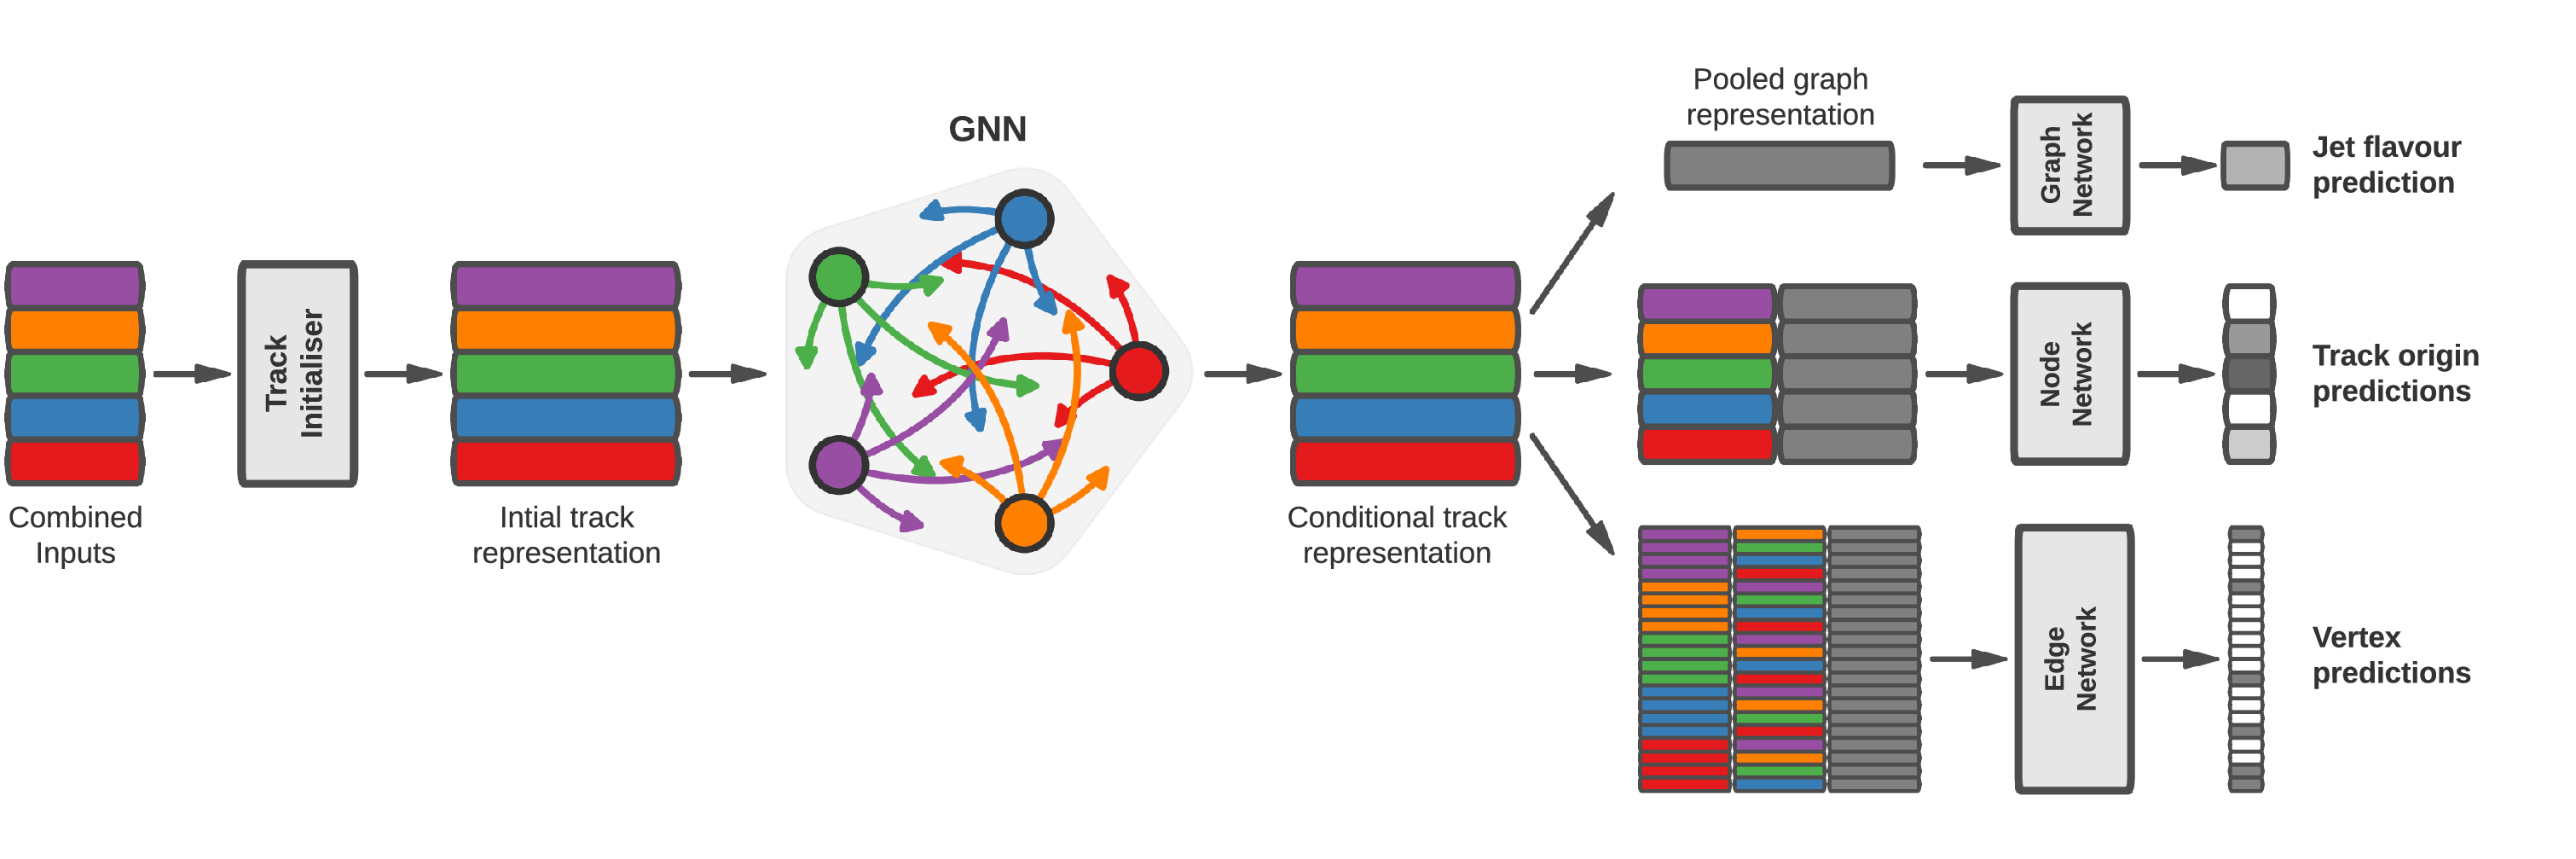
\includegraphics[width=0.99\textwidth]{Images/FTAG/GN/Intro/gnn_architecture.png}
  \caption{The architecture of the GN1 network, from \cite{ATL-PHYS-PUB-2022-027}. The combined input is made of the set of tracks, each of which is given a copy of the two jet variables in addition to the track features as per Table \ref{tab:gnInputVariables}. After a first embedding taking the input to an enriched latent representation, a fully connected graph is defined with the embedded tracks as nodes. The output of the graph is a conditional representation that is used in the three training objectives.} 
  \label{fig:gnnArchitecture}
\end{figure}

A fully-connected graph is built with the embedded track representation as nodes. For the purpose of this section, each of the nodes of the graph are labelled as $h_i$ with feature vector of dimension 64, and there is one such node per track. The graph network updates the defined graph $G(\mathcal{N})$ into a graph $G'(\mathcal{N}')$, with $\mathcal{N}$ and $\mathcal{N}'$ the set of edges, by aggregating the features of each node $h_i$ and neighbouring nodes $\mathcal{N}_i$ using the operation of Ref. \cite{brody2022how}. In more details, the following 4 steps are applied for a single graph update \cite{ATL-PHYS-PUB-2022-027}:
\begin{enumerate}
  \item Each node feature vector is passed through a fully connected layer $W$ producing an updated representation $W\,h_i$ of size 64.
  \item Pairwise scalar edge scores are computed for each pair of nodes $i$ and $j \in \mathcal{N}$: 
  \begin{equation}
    e\left(h_i, h_j\right) = V^T \theta [Wh_i, Wh_j],
  \end{equation}
  where $V$ is a second fully-connected feed-forward layer of size 128, $\theta$ is the \gls{relu} activation function, and $[,]$ stands for the concatenation operation. 
  \item Attention weights are derived from the pairwise edge scores, using a softmax over all $j$ per node $h_i$:
  \begin{equation}
    a_{i,j} = \textrm{softmax}_j\left(e(h_i, h_j)\right).
  \end{equation}
  \item The final step is to aggregate the information to update each node $h_i$ into $h'_i$ by computing the attention weighted sum over each node representation: 
  \begin{equation}
    h'_i = \sum_j a_{i,j} \,.\, W h_j.
  \end{equation} 
\end{enumerate}

For \gls{gn1}, 2 heads attention with 3 such graph network layers applied in succession were found to deliver optimal performance and no overtraining. The output of the graph network is said to be a conditional track representation as it combines each track representation and its neighbours. The ordering of the conditional tracks is kept similar to that of the original track to support matching of track to their truth information. Furthermore, a global reperesentation is derived by combinijng the conditional track representation with learnable attention weights. This rich conditional and global representations can then be used as inputs for the three objectives, implemented with three distrinct feed-forward neural networks \cite{ATL-PHYS-PUB-2022-027}:
\begin{enumerate}
  \item Jet flavour prediction: performed by a graph classification network fed the global representation only. The primary objective of predicting the jet flavour is done by this network, composed of 4 hidden layers with 128, 64, 32, and 16 neurons respectively, finishing on an output of size 3 with softmax for $b$-, $c$-, and light-jet probabilities (size 4 if $\tau$ are included).
  \item Track origin prediction: performed by a node classifier processing each conditional track representation with the global representation. This network is built with three layers of reducing size 128, 64, and 32 to finish on the output layers of size 7 with sotmax, matching the 7 classes corresponding to the different truth origins.
  \item Vertex prediction: performed by a nodes pairs binary classifier that receives every possible combinations of representational tracks as well as the global representation. This network is also made of 3 layers of size 128, 64, and 32 for a final output of size 1 with sigmoid, stating whether the pair of tracks have a common vertex. 
\end{enumerate}

The architecture of \gls{gn1} is an enhanced version of \gls{dips}, with the track initialiser and graph classifiers corresponding to $\Phi$ and $F$. Added elements are the powerful \gls{gnn} layers and conditional representation pooling layer with attention, as well as the auxiliary objectives. \\

Training \gls{gn1} involves minimising the combining objective $\mathcal{L}_{\textrm{total}}$ of Equation \ref{eq:totalobjgn} \cite{ATL-PHYS-PUB-2022-027}. $\mathcal{L}_{\textrm{flavour}}$ is the categorial cross entropy loss, as defined in Equation \ref{eq:statEntropy}, over the different jet flavours to output the per flavour probabilities. $\mathcal{L}_{\textrm{track}}$ is the categorial cross entropy loss for the track origin prediction averaged over all tracks in a batch. Due to intrinsic differences in the relative frequency of track origins, the contribution of each origin is weighted by their inverse frequency of occurence. Finally, $\mathcal{L}_{\textrm{vertex}}$ is the binary cross-entropy of the track-pair compatibility averaged over all track-pairs in a batch. The importance of matching tracks from $b$- and $c$-hadron is artificially increased by giving them double the weight compared to other track-pairs.

\begin{equation}\label{eq:totalobjgn}
  \mathcal{L}_{\textrm{total}} = \mathcal{L}_{\textrm{flavour}} + \alpha \, \mathcal{L}_{\textrm{track}} + \beta \, \mathcal{L}_{\textrm{vertex}}.
\end{equation}

In Equation \ref{eq:totalobjgn}, weights are applied to combine the different tasks that are represented by distinct values, reflecting their specific loss functions and difficulties. Weights of $\alpha = 0.5$ and $\beta = 1.5$ \cite{ATL-PHYS-PUB-2022-027} where found to lead the auxiliary objectives to converge to similar values, giving them equal weighting in $\mathcal{L}_{\textrm{total}}$. The proposed choice for these parameters also let the primary objective $\mathcal{L}_{\textrm{flavour}}$ dominate the global loss, and small variations of $\alpha$ and $\beta$ were not found to significantly impact the performance. The results presented here come from Ref \cite{ATL-PHYS-PUB-2022-027}, where a \gls{gn1} models were trained for 100 epochs with a 30 million jets sample made of 60\% $t\bar{t}$ and 40\% $Z'$, as previously described in this chapter. The validation loss on a statistically independent sample of 500k jets is monitiored, with the epoch minimising it selected for further analysis. The optimiser is based on Adam \cite{adamPaper} with a learning rate of $1e-3$ and a batch size of 4000 jets spread across 4 \gls{gpu}. \\

The results of the training are presented in Figures \ref{fig:GN1rocb} and \ref{fig:GN1rocc} for $b$- and $c$-tagging respectively, where a \gls{dl1r} model retrained on similar inputs to the GN1 with 75 million jets is presented as reference, with a significant caveat being the lack of retraining of the input \gls{rnnip} sub-tagger. The \gls{roc} curves of a GN1 model given an additional track input to those of Table \ref{tab:gnInputVariables} indicating if a track was used in the reconstruction of an electron or a muon is also included as GN1 Lep. At the time of deriving these results, the \gls{dl1d} tagger was yet not officially released and is thus not included. Its performance can be estimated at roughly 20\% to 50\% above \gls{dl1r}, far from the observed gains made by the \gls{gn1} models - as was also displayed in Figures \ref{fig:DL1dshapc} and \ref{fig:DL1dshapb}. 

\begin{figure}[h!]
  \centering
  \begin{subfigure}[b]{0.98\textwidth}
      \centering
      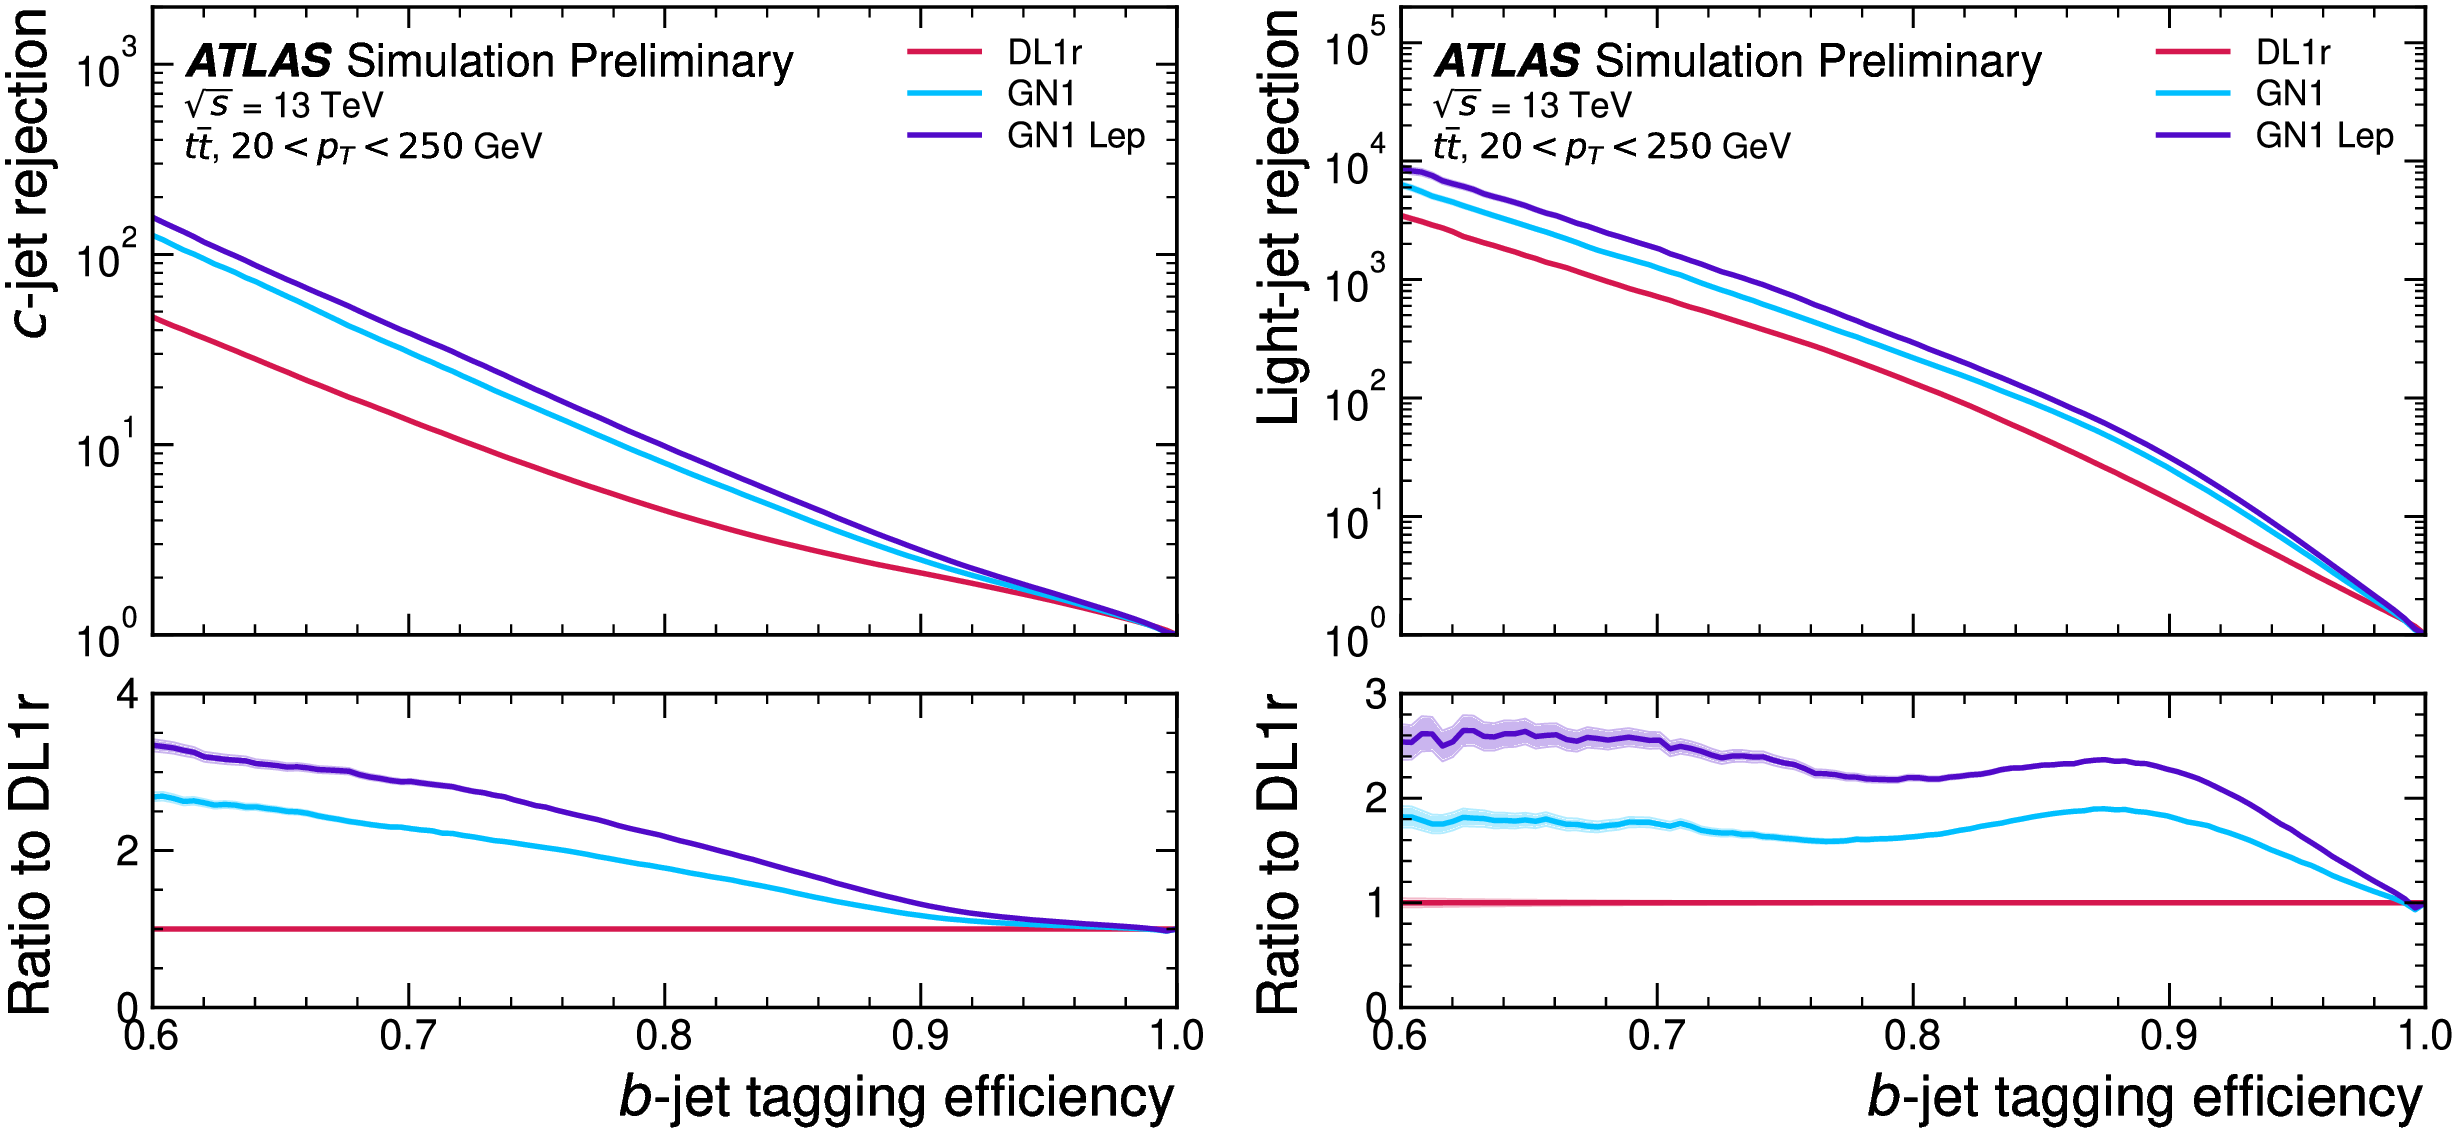
\includegraphics[width=0.98\textwidth]{Images/FTAG/GN/GN1/ROC/ttb.png}
      \caption{GN1 and DL1r performance on the $t\bar{t}$ test sample, with $20 < p_T < 250$ GeV.} 
      \label{fig:GN1ttb}
  \end{subfigure}\\
  \begin{subfigure}[b]{0.98\textwidth}
    \centering % UNreadable: increase font size
      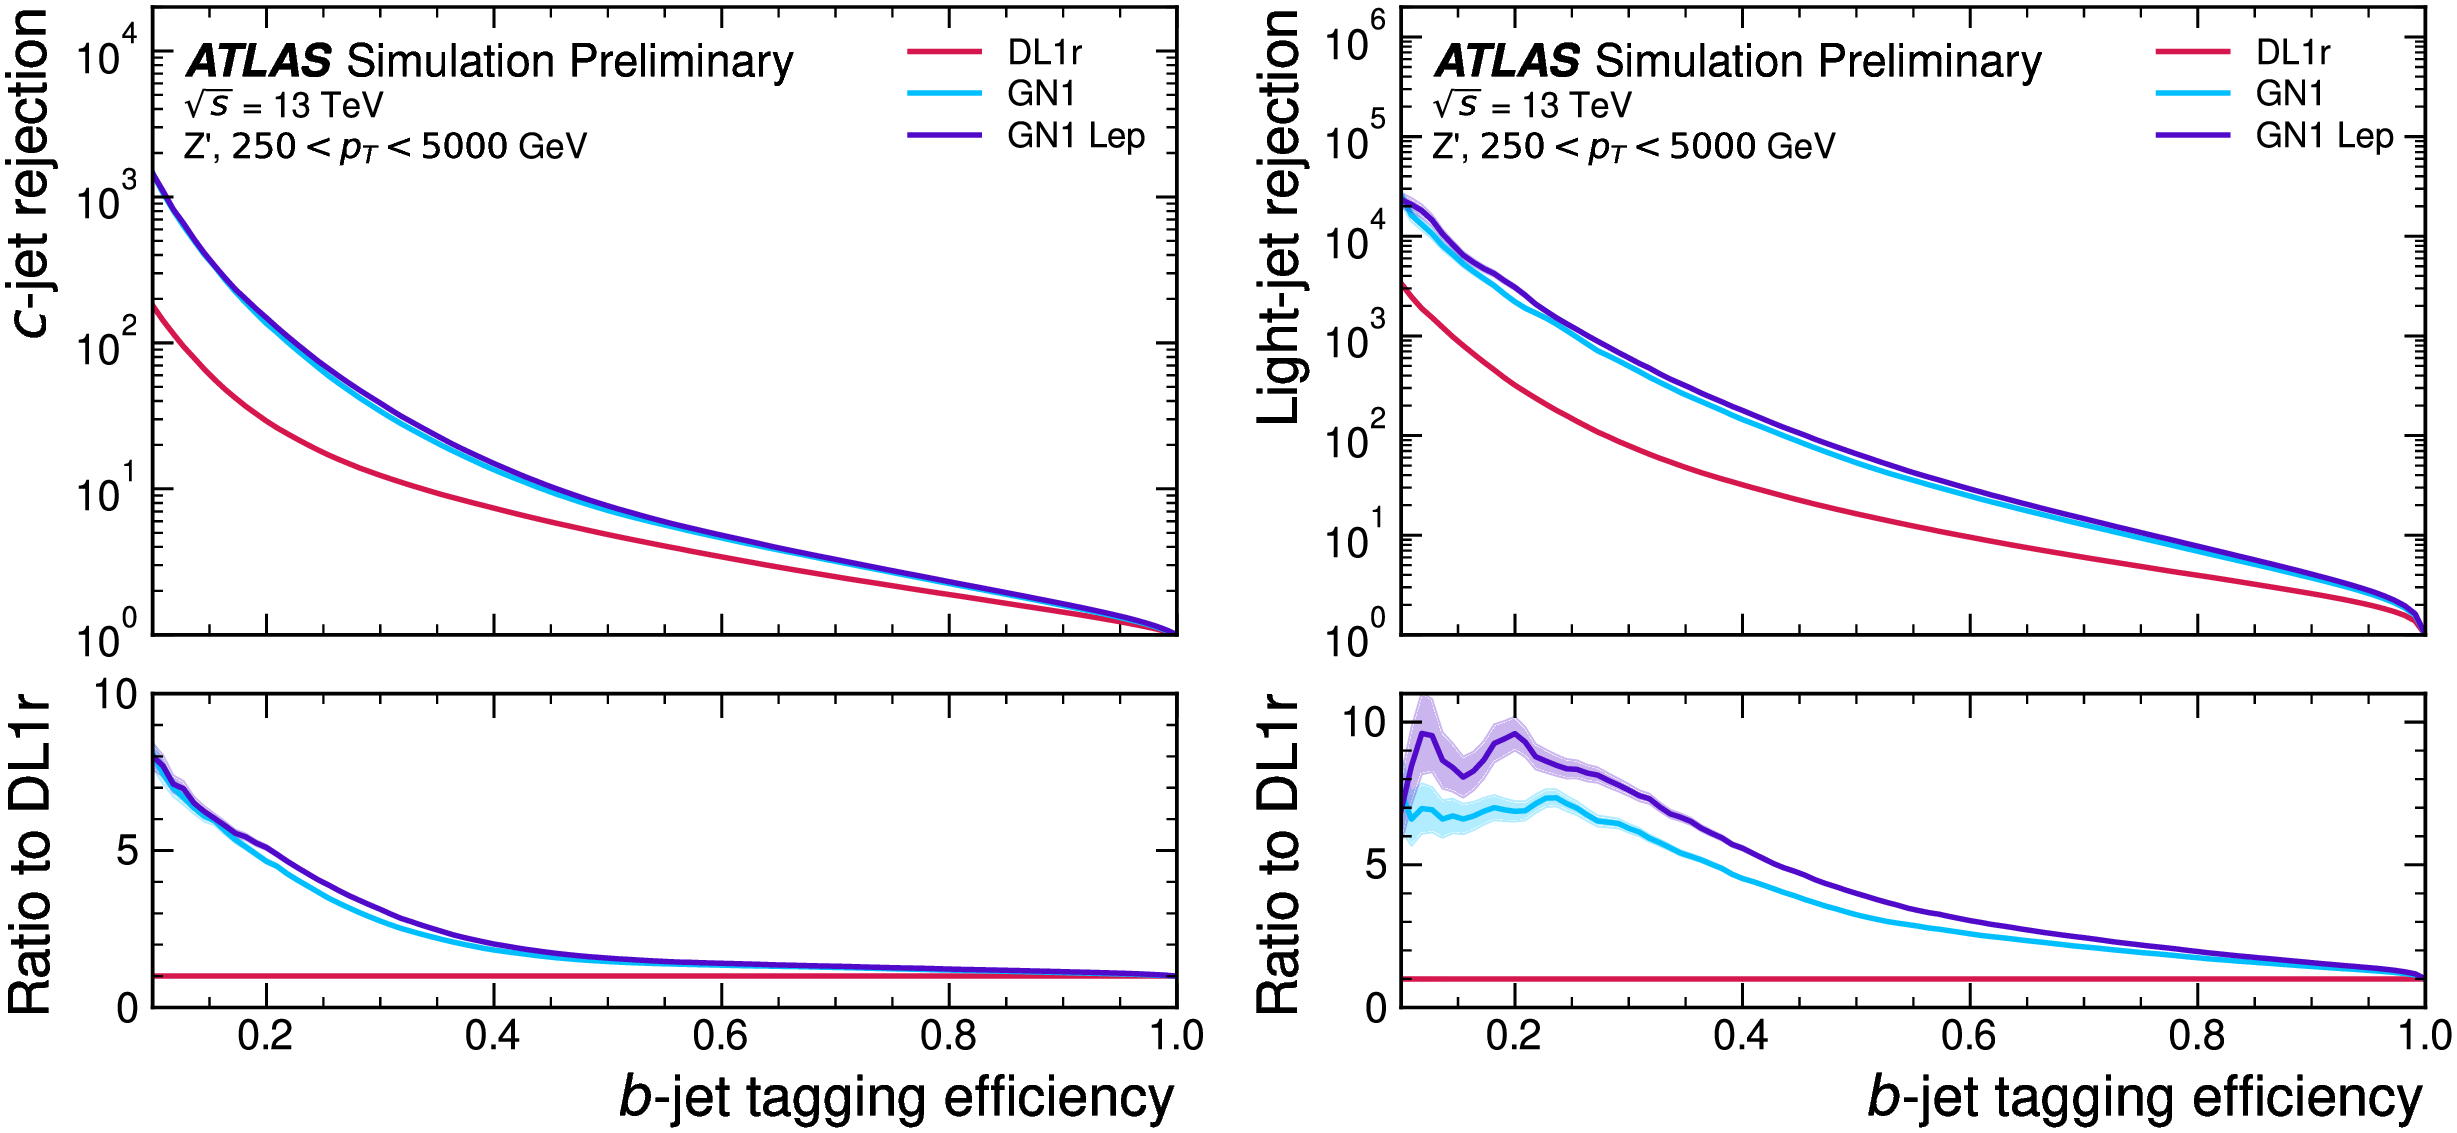
\includegraphics[width=0.98\textwidth]{Images/FTAG/GN/GN1/ROC/zpb.png}
      \caption{GN1 and DL1r performance on the $Z'$ test sample, with $250 < p_T < 5000$ GeV.} 
      \label{fig:GN1zpb}
  \end{subfigure}
  \caption{ROC curves tracing the $b$-tagging efficiency versus the $c$-jet (left) and light-jet (right) rejections for the $t\bar{t}$ (top) and $Z'$ (bottom) test samples, from \cite{ATL-PHYS-PUB-2022-027}. Models compared are DL1r in red, GN1 in blue, and GN1 Lep in purple. The bottom panels show the ratio with respect to DL1r. The flavour fraction is set at $f^b_c = 0.018$ for DL1r and 0.05 for GN1 and GN1 Lep. The binomial error bands are shown as shaded regions.}
  \label{fig:GN1rocb}
\end{figure} 

Most of the improvement in rejections made by \gls{gn1} models can be found a lower tagging efficiencies. At the typical working point of 70\% on the low $p_T$ region defined by $t\bar{t}$, the $c$-jet (light-jet) rejection is 110\% (80\%) above that of \gls{dl1r}. Gains are observed across the considered $p_T$ spectrum, with a gain of 180\% (500\%) at a working point of 30\% - the 30\% working point on $Z'$ corresponds to using the 70\% working point on $t\bar{t}$. The \gls{gn1} version with lepton information further improves the performance, to a $c$-rejection (light-rejection) of 180\% (150\%) at the 70\% \gls{wp} on $t\bar{t}$ and 180\% (600\%) on the $Z'$ at the 30\% \gls{wp}. Part of the measured performance increase with \gls{gn1} is due to the looser track selections leveraged by \gls{gn1} and to a more sophisticated exploitation of the noisy low-level track information. The \gls{gn1} and \gls{dl1r} discriminants for $b$-tagging are presented in Figure \ref{fig:GN1disb}. The distributions for \gls{gn1} moves the $b$-jet distribution to higher values of the discriminants, indicating a higher confidence on the associated $p_b$. \\

\begin{figure}[h!]
  \centering
  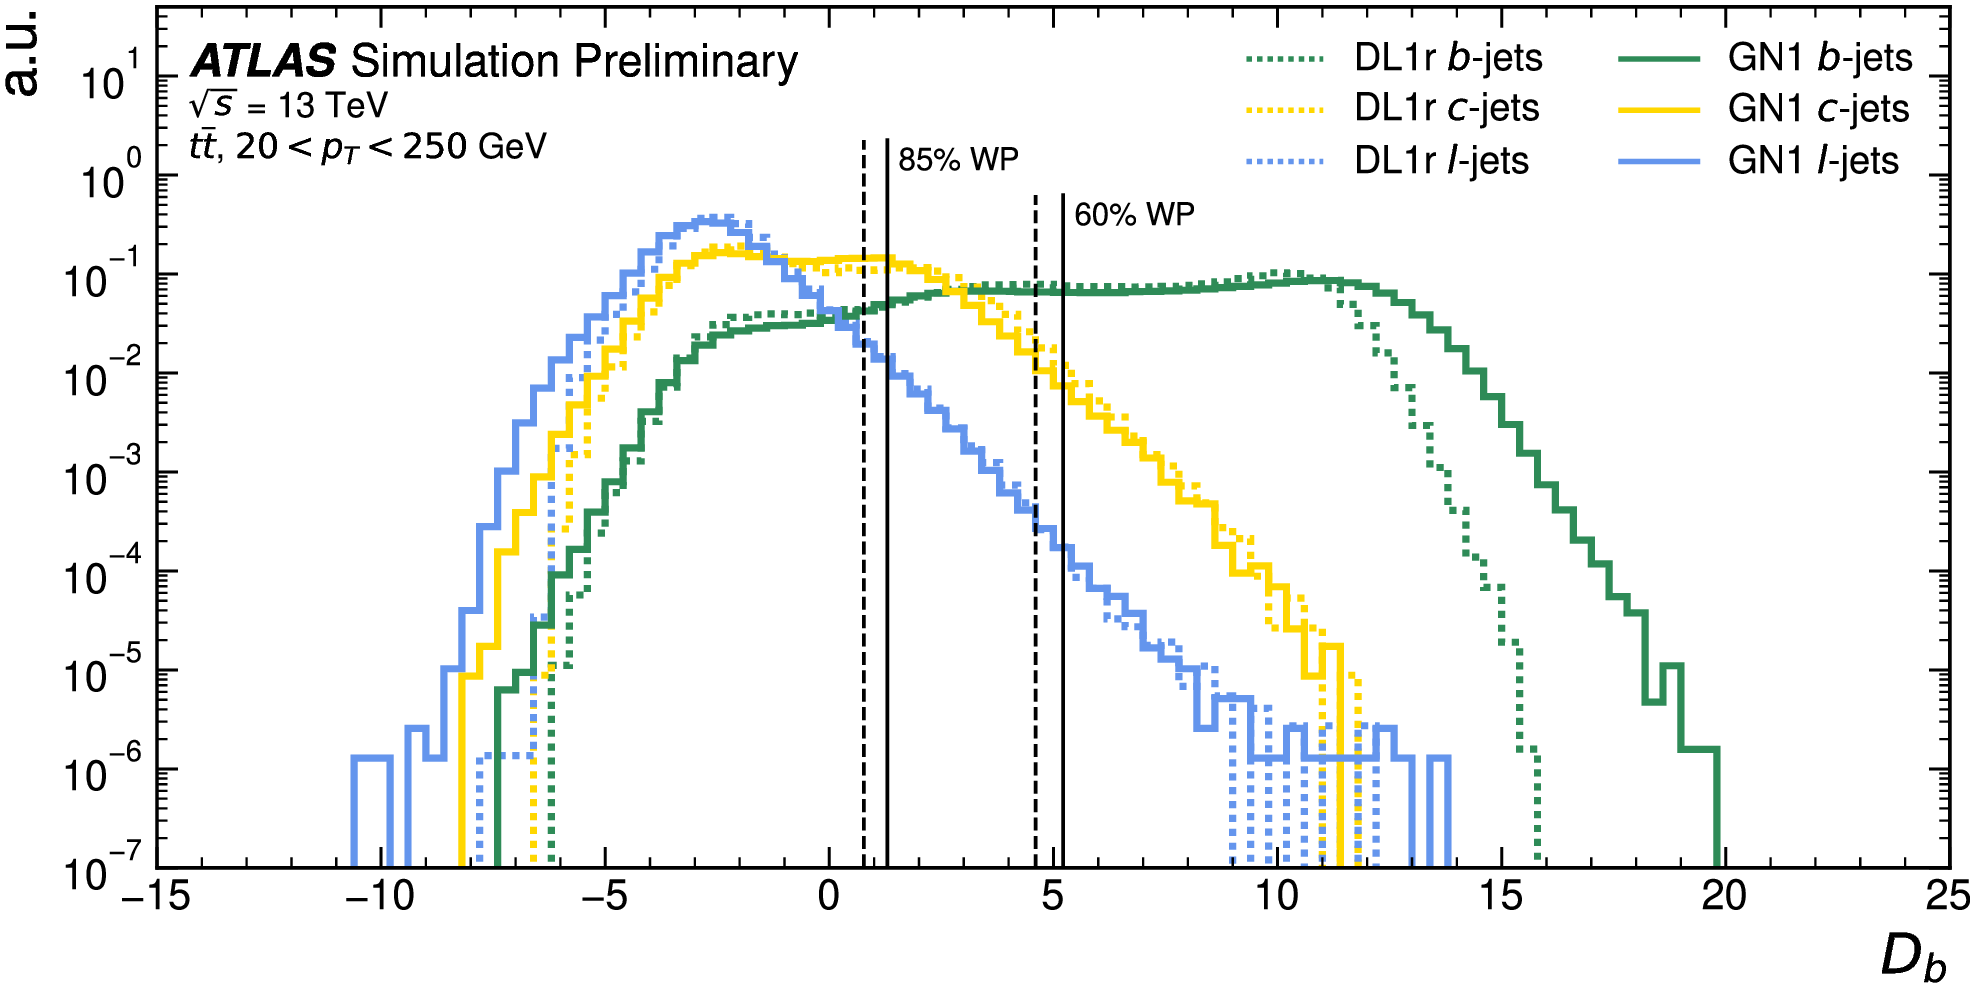
\includegraphics[width=0.8\textwidth]{Images/FTAG/GN/GN1/eff/ttb.png}
  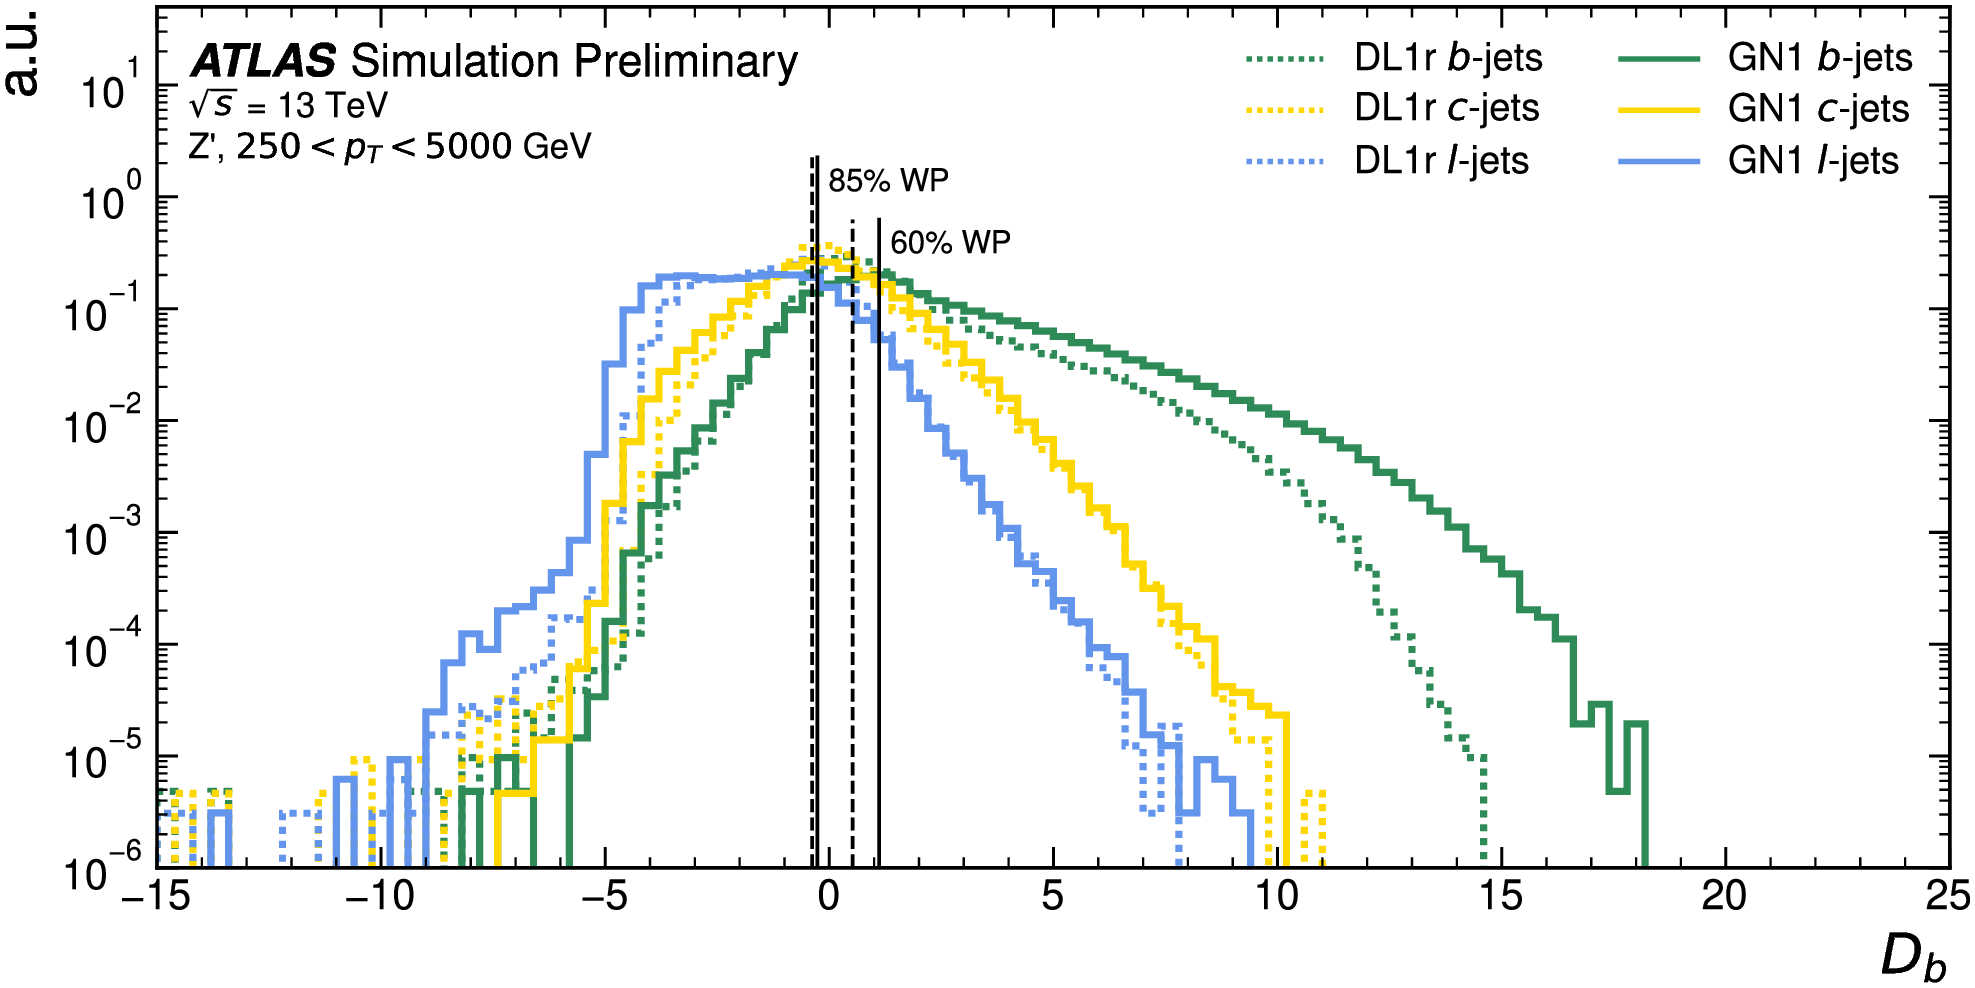
\includegraphics[width=0.8\textwidth]{Images/FTAG/GN/GN1/eff/zpb.png}
  \caption{Comparing the GN1 and DL1r $b$-tagging discriminants $D_b$ normalised distributions on the $t\bar{t}$ (top) and $Z'$ (bottom) test samples, from \cite{ATL-PHYS-PUB-2022-027}. Models compared are DL1r in dashed lines and GN1 in continuous line. Each flavour is indicated by a different colour: green for $b$-jets, yellow for $c$-jets, and blue for light-jets. The flavour fraction is set at $f^b_c = 0.018$ for DL1r and 0.05 for GN1}
  \label{fig:GN1disb}
\end{figure} 

The $c$-tagging performance is presented in Figures \ref{fig:GN1rocc} and \ref{fig:GN1disc}, displaying the \gls{roc} curves and $c$-tagging discriminant distributions $D_c$. \gls{gn1} significantly outperforms \gls{dl1r} for $c$-tagging: both background rejections are doubled on the $t\bar{t}$ sampled at a $c$-tagging \gls{wp} of 25 \%, with a more modest increase on the $Z'$ sample of 60\% for $b$-rejection and 100\% for light-rejection at the same $c$-jet \gls{wp}.

\begin{figure}[h!]
  \centering
  \begin{subfigure}[b]{0.98\textwidth}
      \centering
      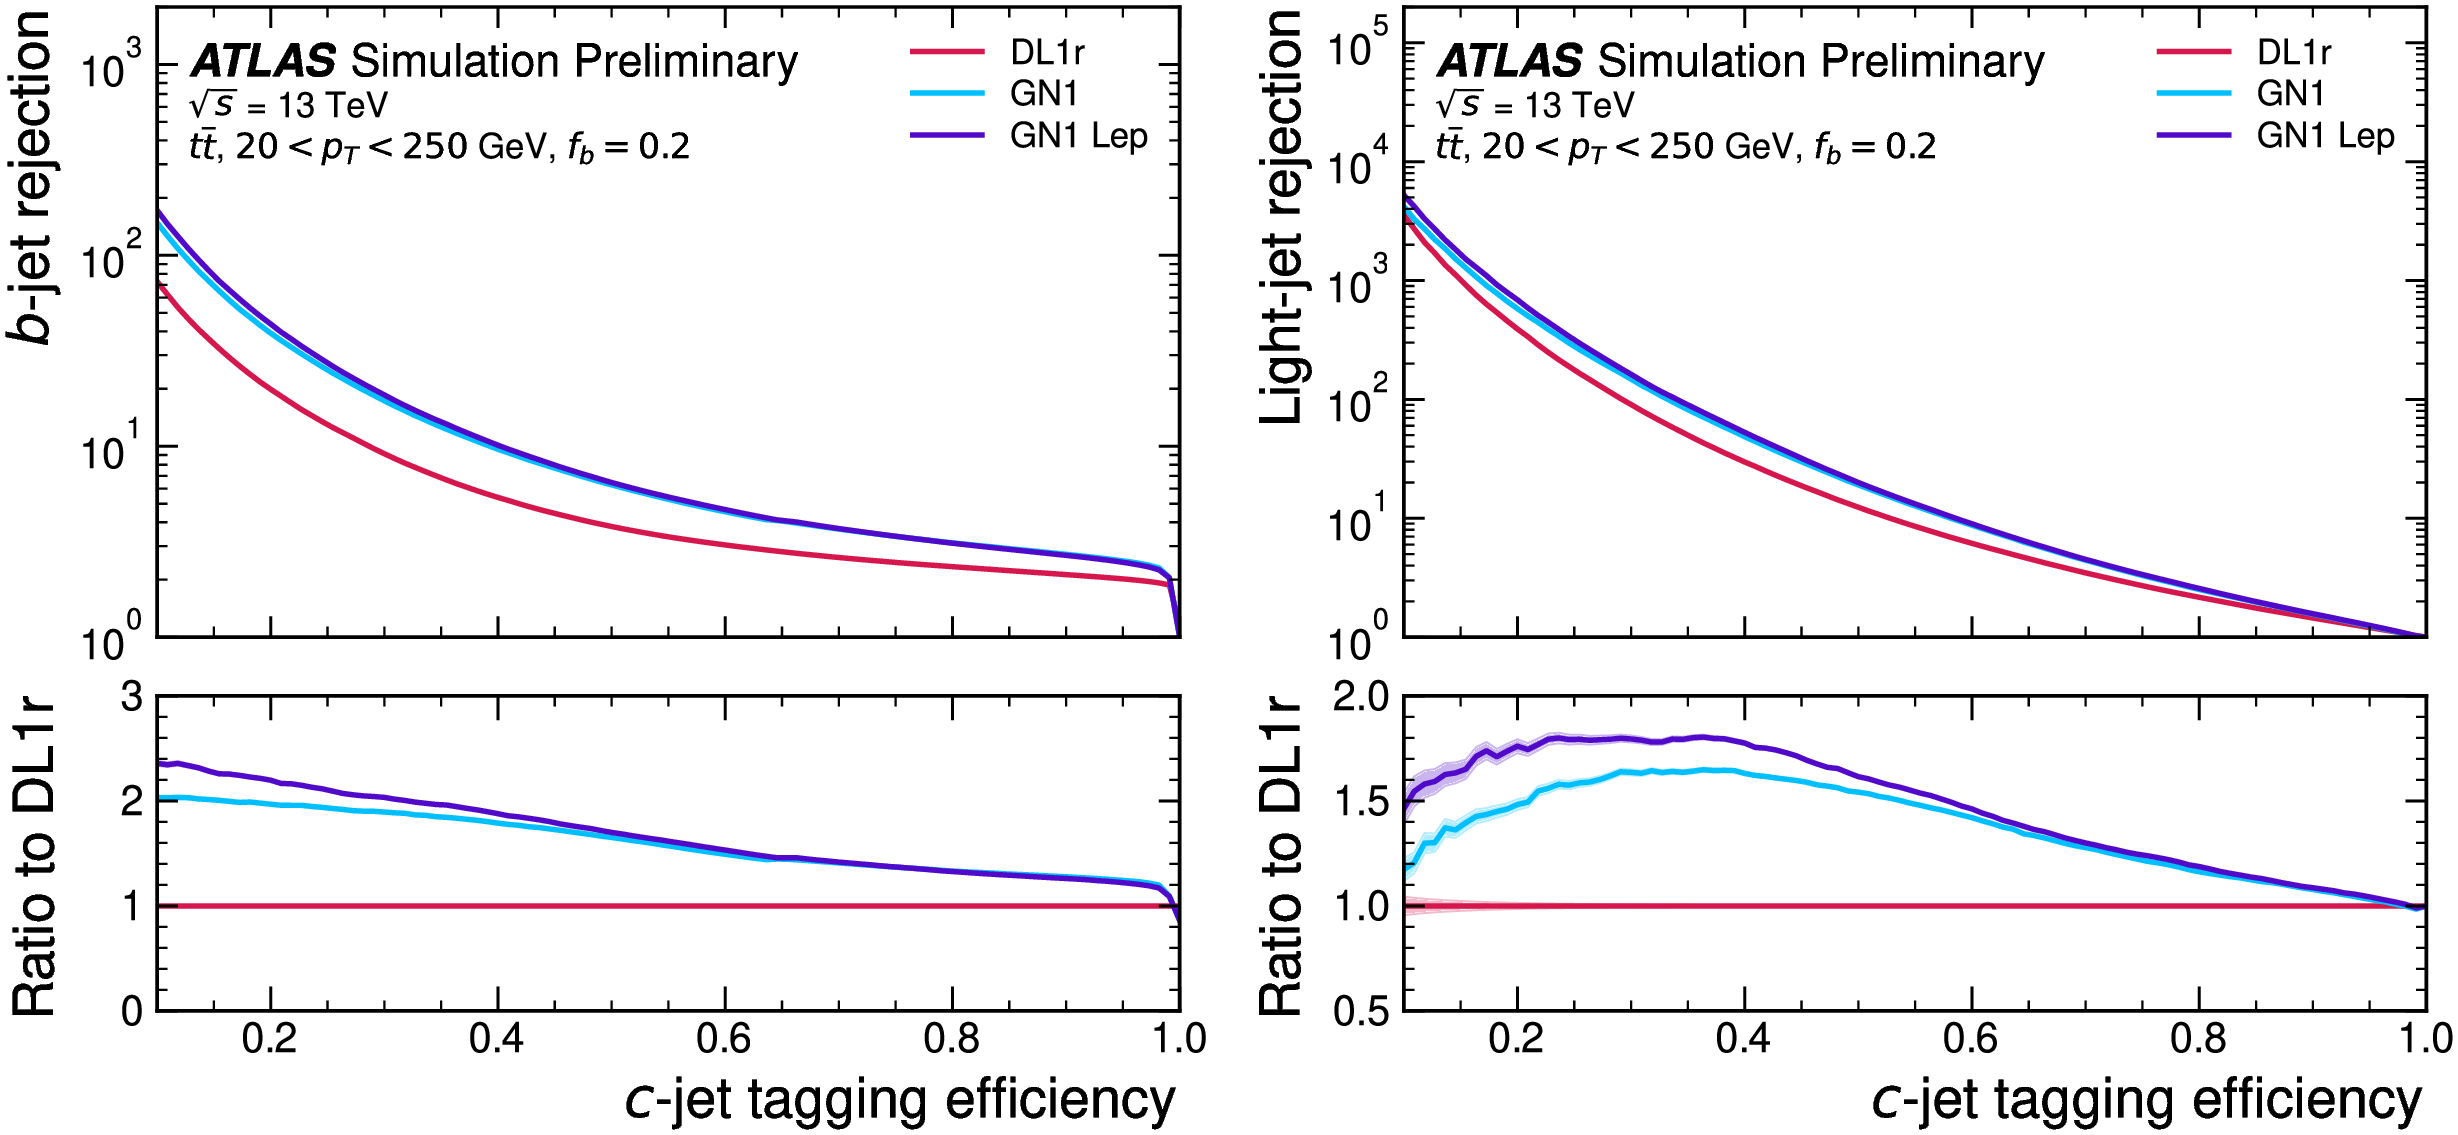
\includegraphics[width=0.98\textwidth]{Images/FTAG/GN/GN1/ROC/ttc.png}
      \caption{GN1 performance on the $t\bar{t}$ test sample, with $20 < p_T < 250$ GeV.} 
      \label{fig:GN1ttc}
  \end{subfigure}\\
  \begin{subfigure}[b]{0.98\textwidth}
    \centering % UNreadable: increase font size
      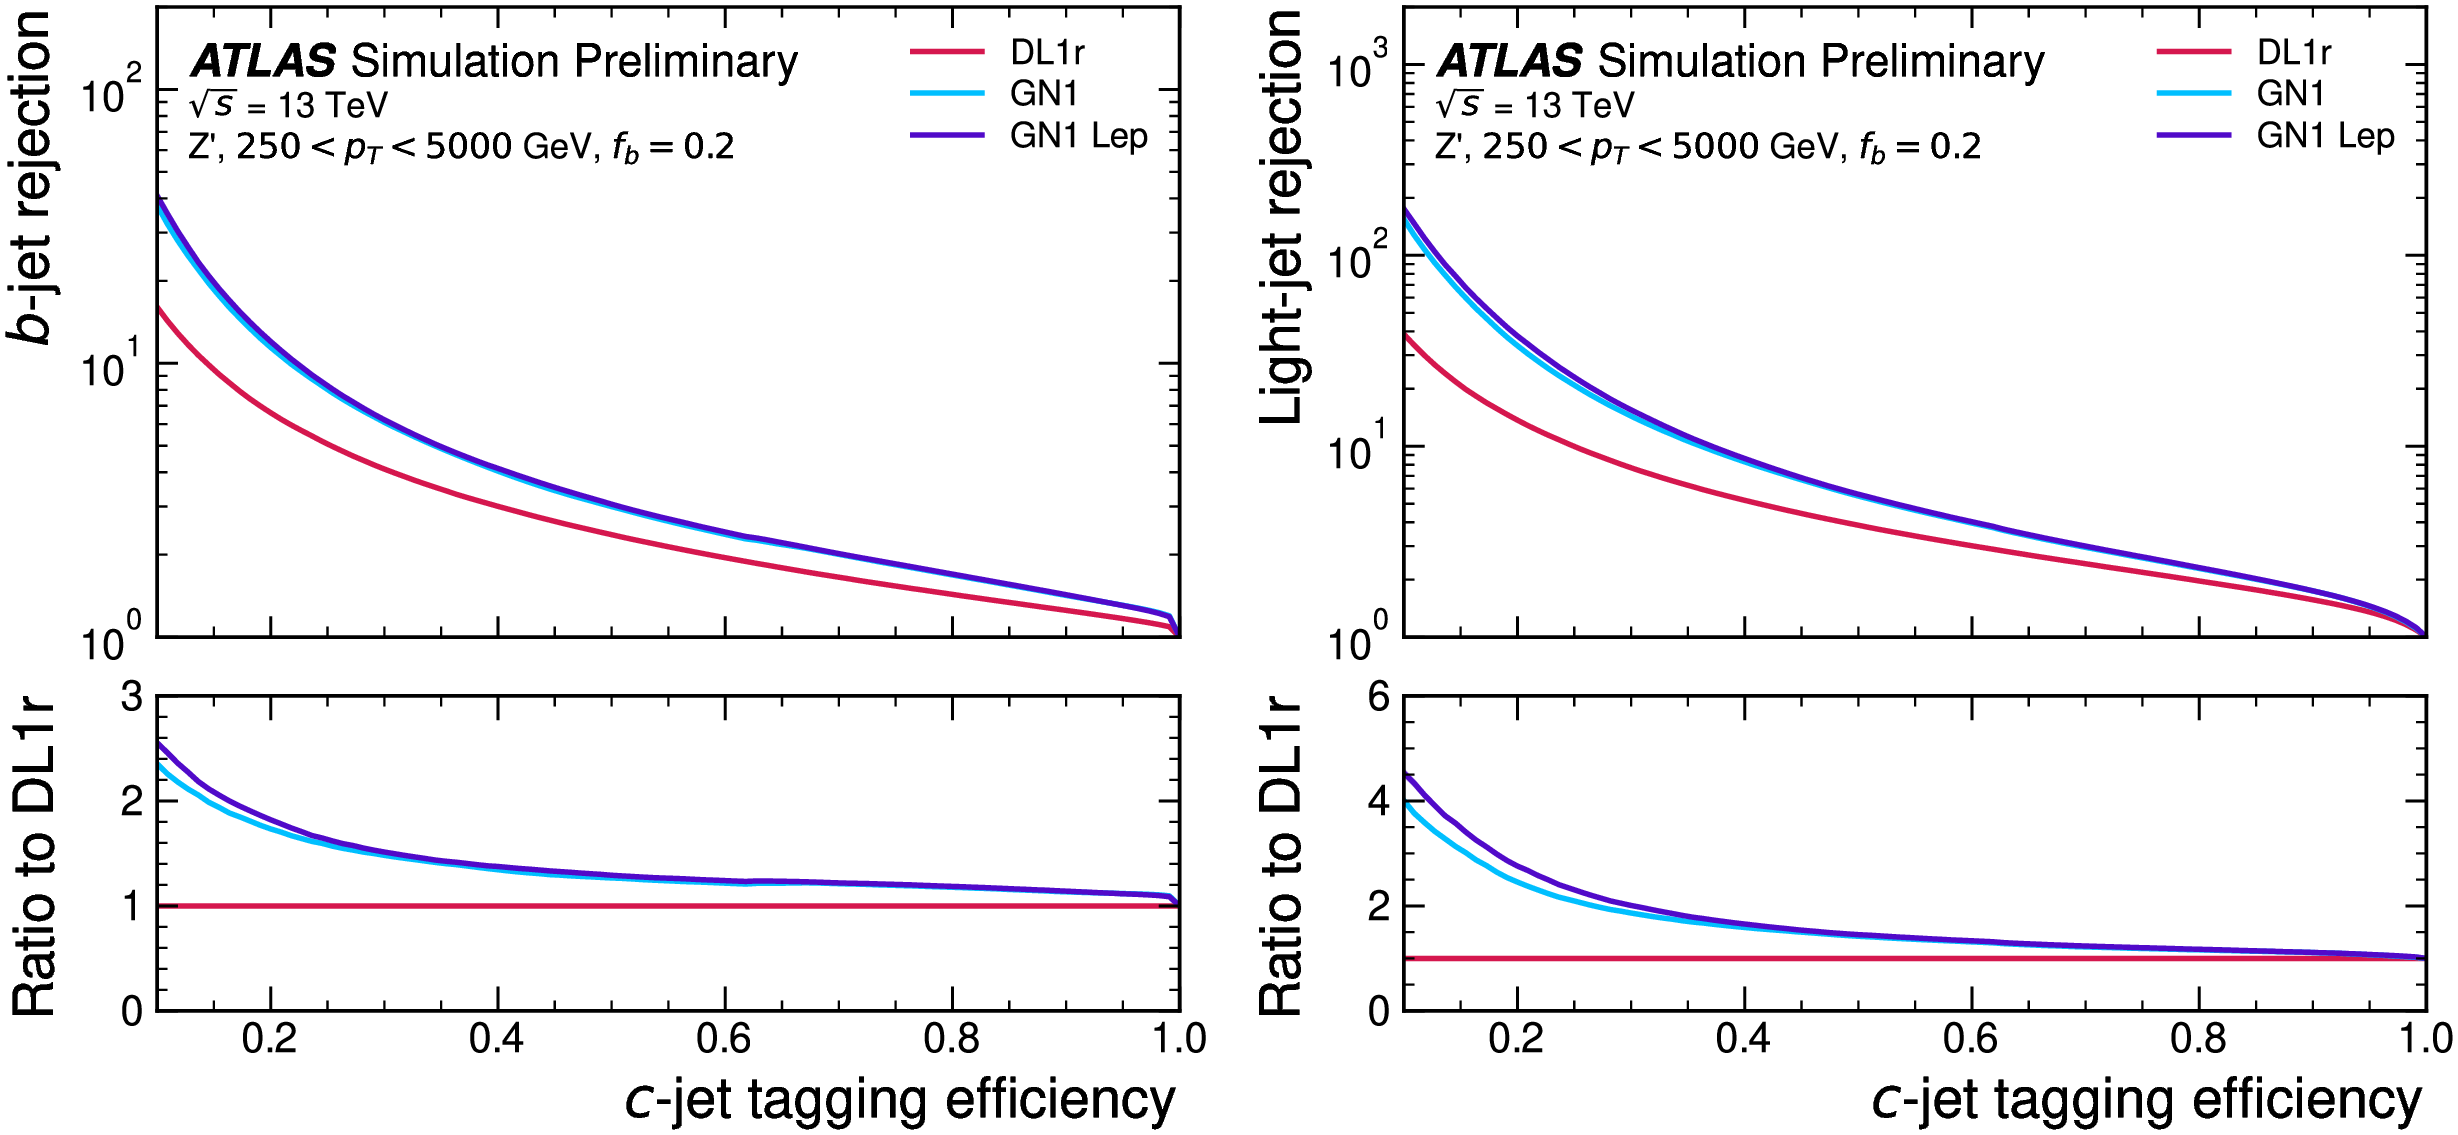
\includegraphics[width=0.98\textwidth]{Images/FTAG/GN/GN1/ROC/zpc.png}
      \caption{GN1 performance on the $Z'$ test sample, with $250 < p_T < 5000$ GeV.} 
      \label{fig:GN1zpc}
  \end{subfigure}
  \caption{ROC curves tracing the $c$-tagging efficiency versus the $b$-jet (left) and light-jet (right) rejections for the $t\bar{t}$ (top) and $Z'$ (bottom) test samples, from \cite{ATL-PHYS-PUB-2022-027}. Models compared are DL1r in red, GN1 in blue, and GN1 Lep in purple. The bottom panels show the ratio with respect to DL1r. The flavour fraction is set at $f^c_b = 0.2$. The binomial error bands are shown as shaded regions.}
  \label{fig:GN1rocc}
\end{figure} 

\begin{figure}[h!]
  \centering
  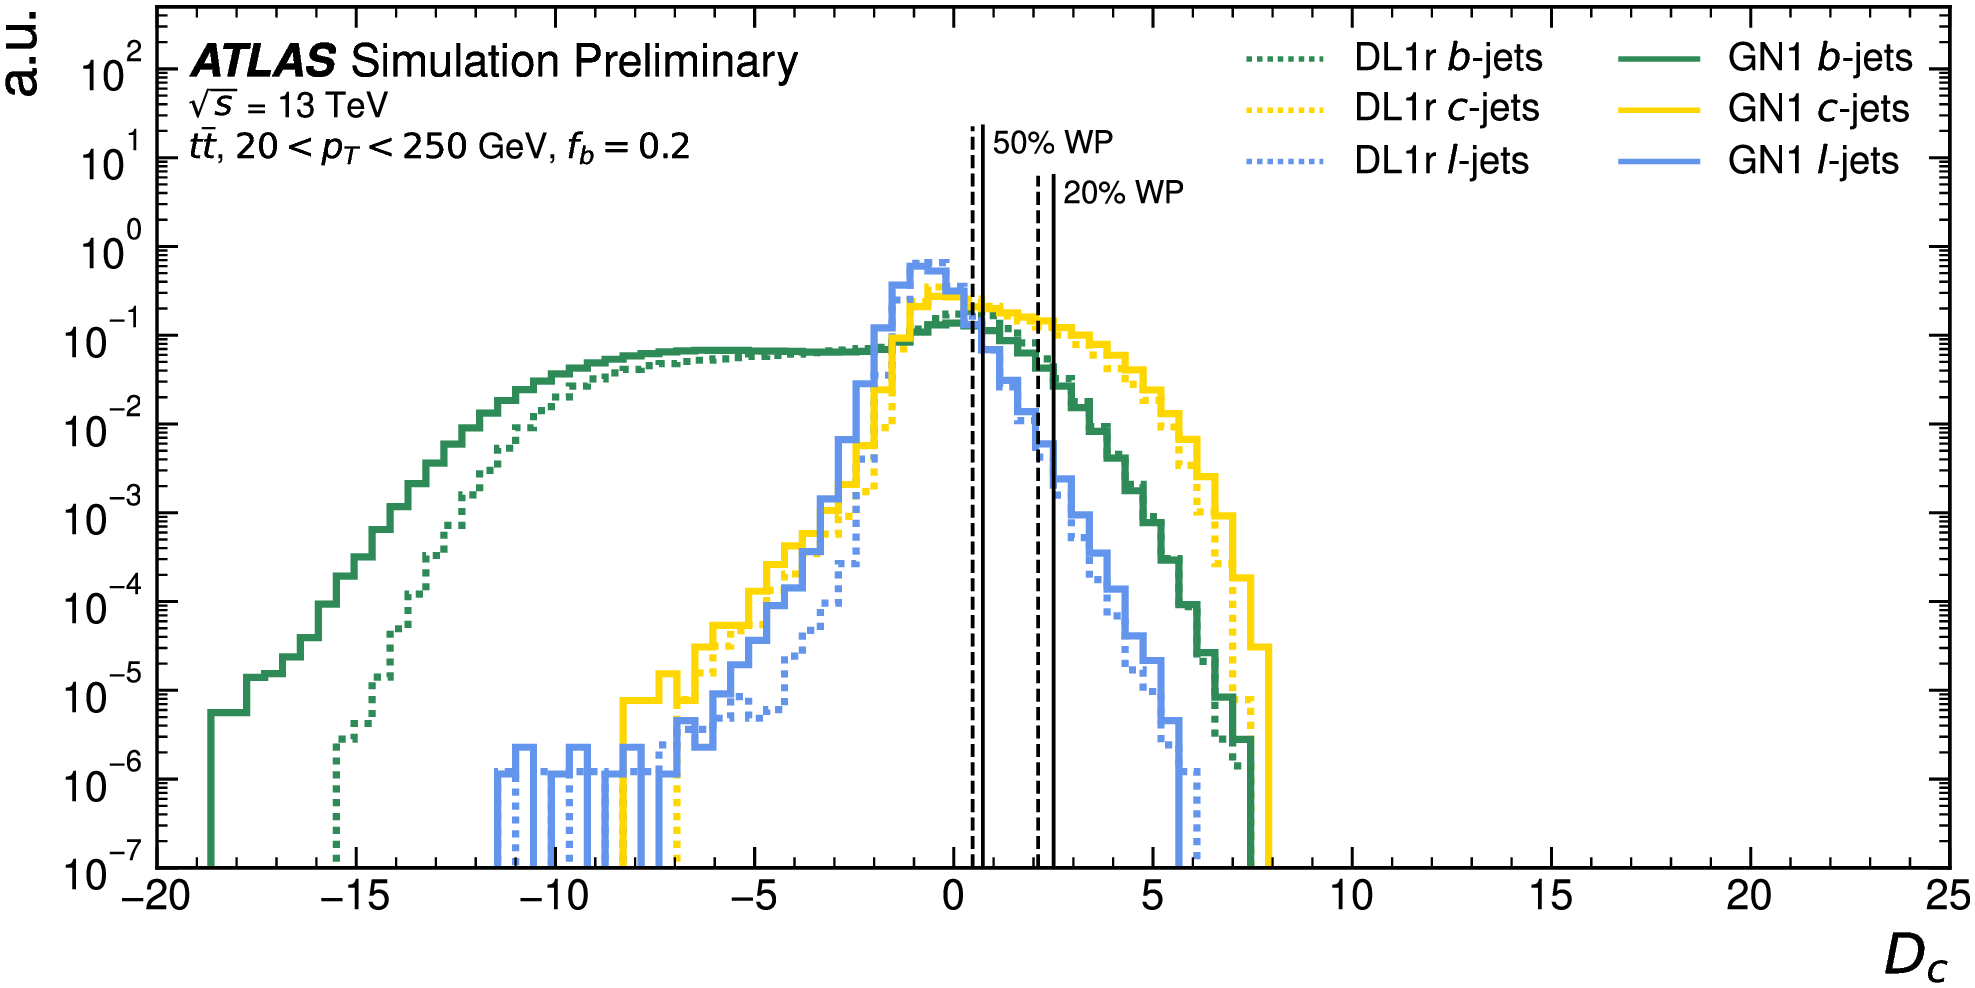
\includegraphics[width=0.8\textwidth]{Images/FTAG/GN/GN1/eff/ttc.png}
  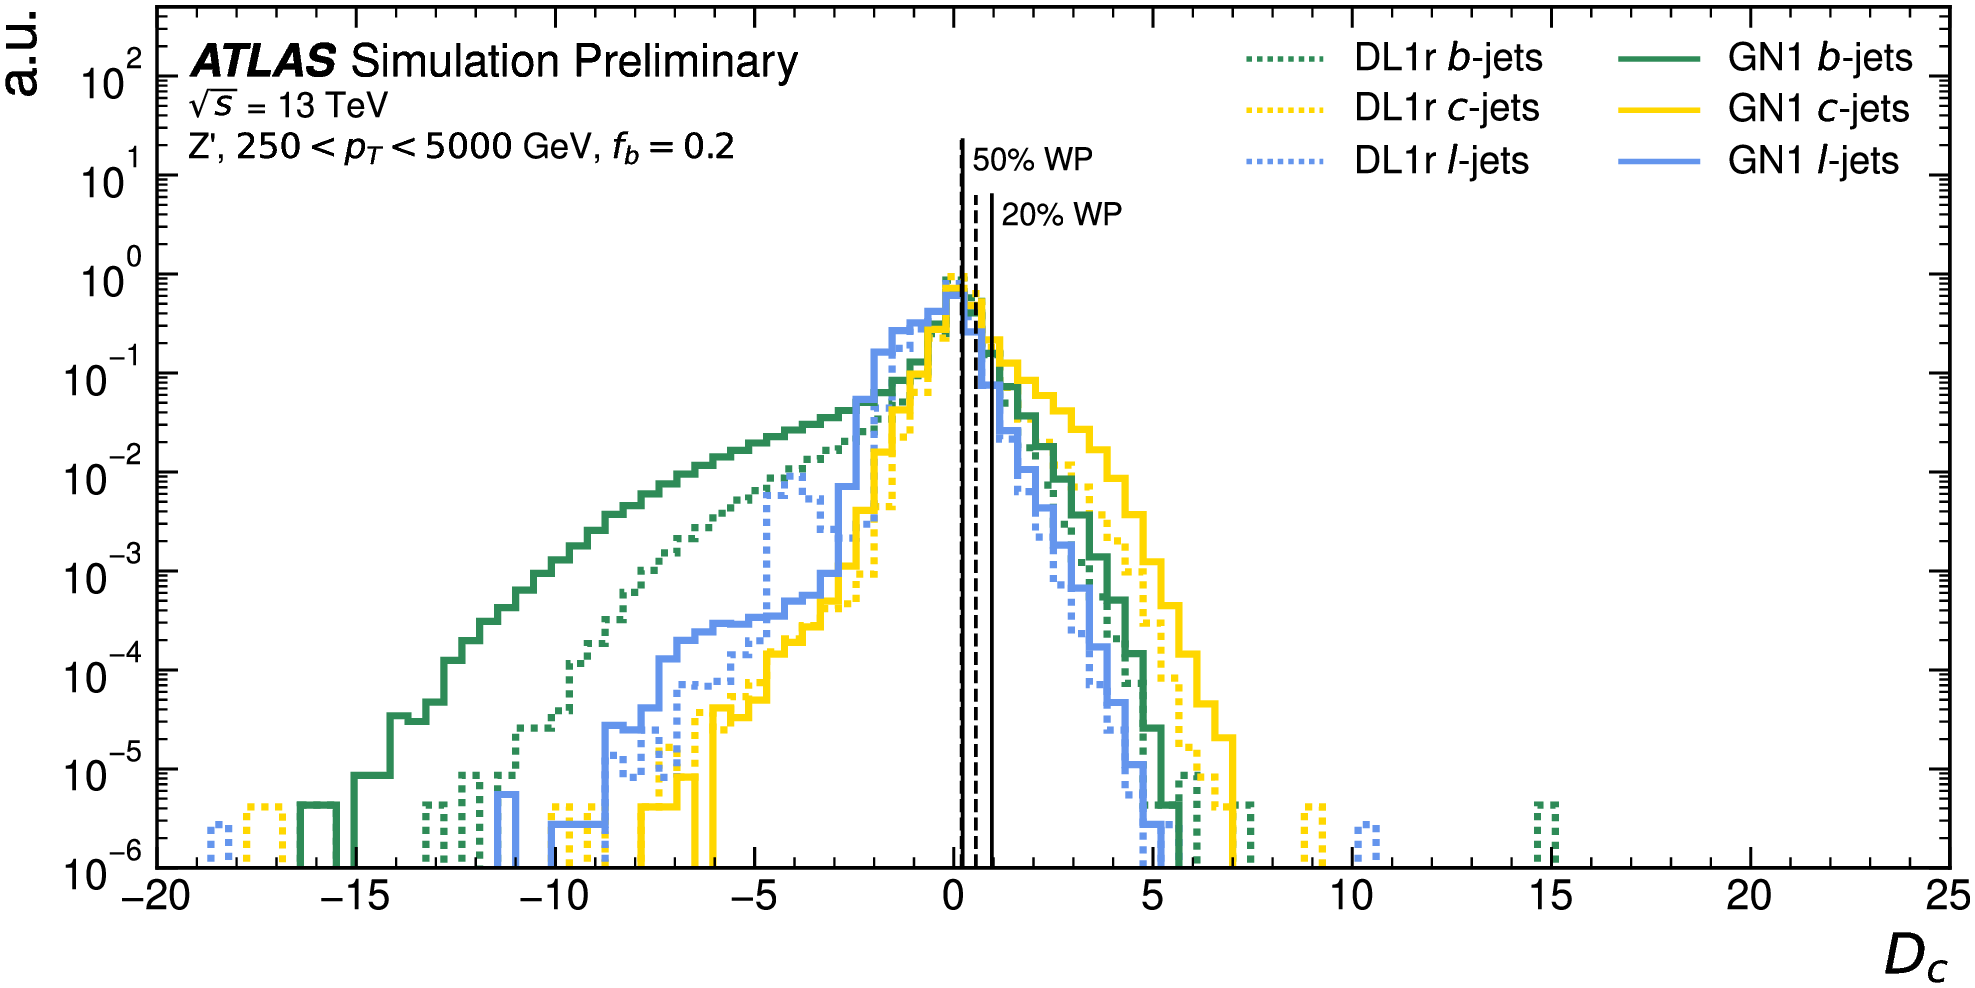
\includegraphics[width=0.8\textwidth]{Images/FTAG/GN/GN1/eff/zpc.png}
  \caption{Comparing the GN1 and DL1r $c$-tagging discriminants $D_c$ normalised distributions on the $t\bar{t}$ (top) and $Z'$ (bottom) test samples, from \cite{ATL-PHYS-PUB-2022-027}. Models compared are DL1r in dashed lines and GN1 in continuous line. Each flavour is indicated by a different colour: green for $b$-jets, yellow for $c$-jets, and blue for light-jets. The flavour fraction is set at $f^c_b = 0.2$.}
  \label{fig:GN1disc}
\end{figure} 

As previously explained, the tagging performance is strongly dependent on the jet energy considered, explaining the observed rejections differences between the $t\bar{t}$ and $Z'$ samples. Higher energies correlate with higher transverse momentum $p_T$. More energy in the system introduces a higher multiplicity of fragmentation particles challenging the reconstruction process. The direction of emission of the particles is more collimated and approaches the resolution power of the tracking detector of fixed granularity: different tracks are no longer individually resolvable and their hits merge. Due to relativistic effect, at higher $p_T$ the time of flight of heavy-hadrons increase, delaying their decay further into the detector. Traces left by the heavy-hadrons paths and fragmentation particles introduce inaccuriacies in the reconstructed track parameters \cite{ATLAS-tracks-algo}. This degradation of the track quality impacts the jet tagging performance significantly, as displayed in Figure \ref{fig:GN1ptb} showing the $b$-tagging efficiency as a function of jet $p_T$ for a fixed light-jet rejection of 100 in each bin. \gls{gn1} outperforms \gls{dl1r} across the studied $p_T$ range, with a very significant $b$-efficiency improvement of a factor $\sim$ 2 at high values of $p_T$ above $2.5$ TeV. 

\begin{figure}[h!]
  \centering
  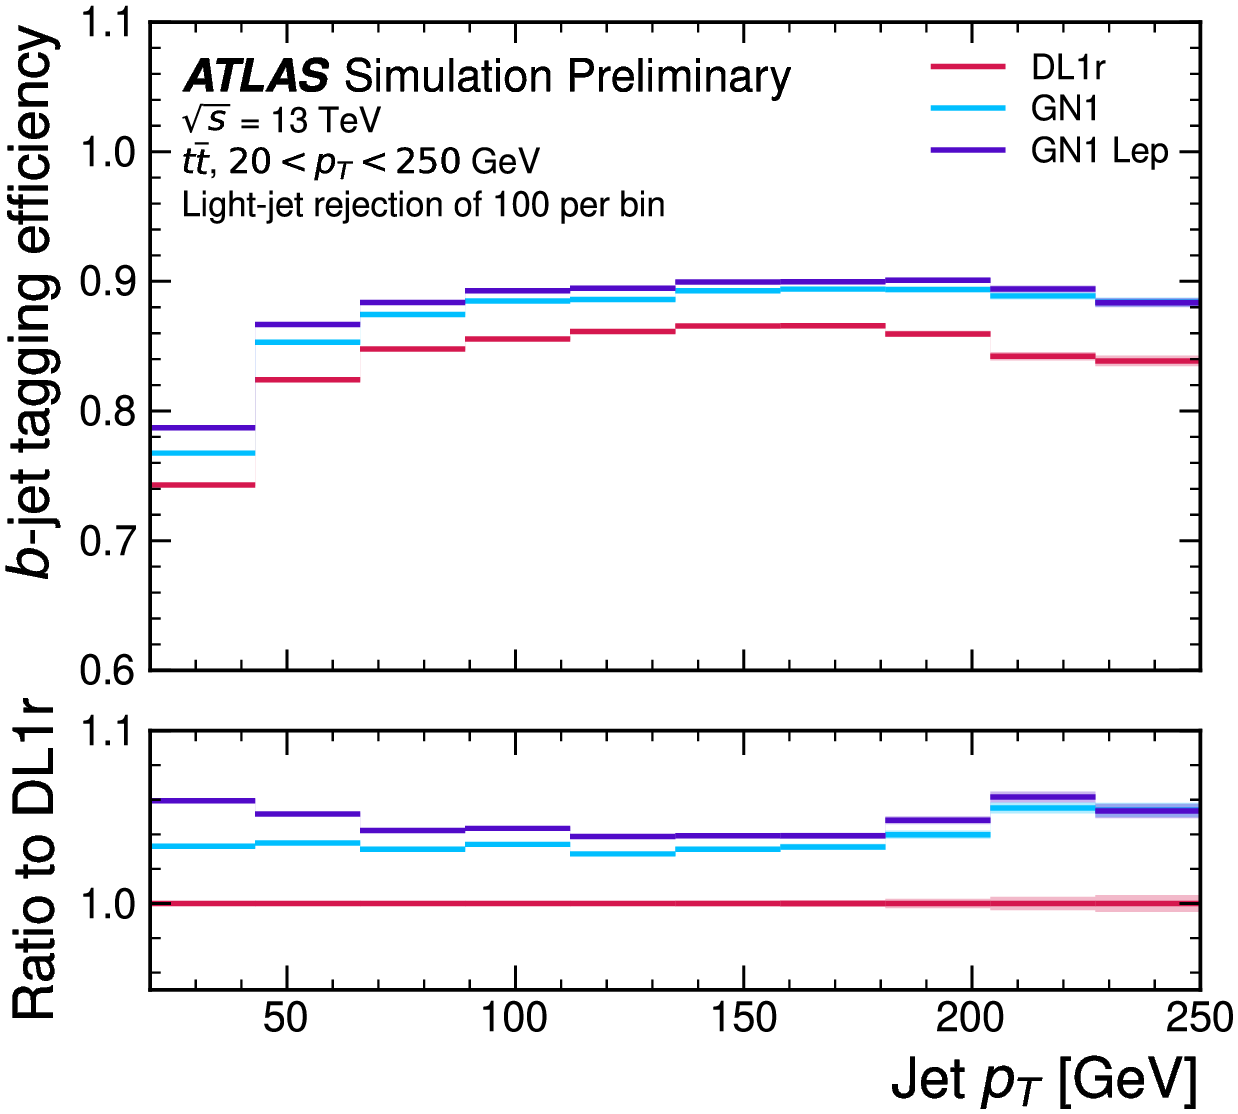
\includegraphics[width=0.45\textwidth]{Images/FTAG/GN/GN1/eff/ptttb.png}
  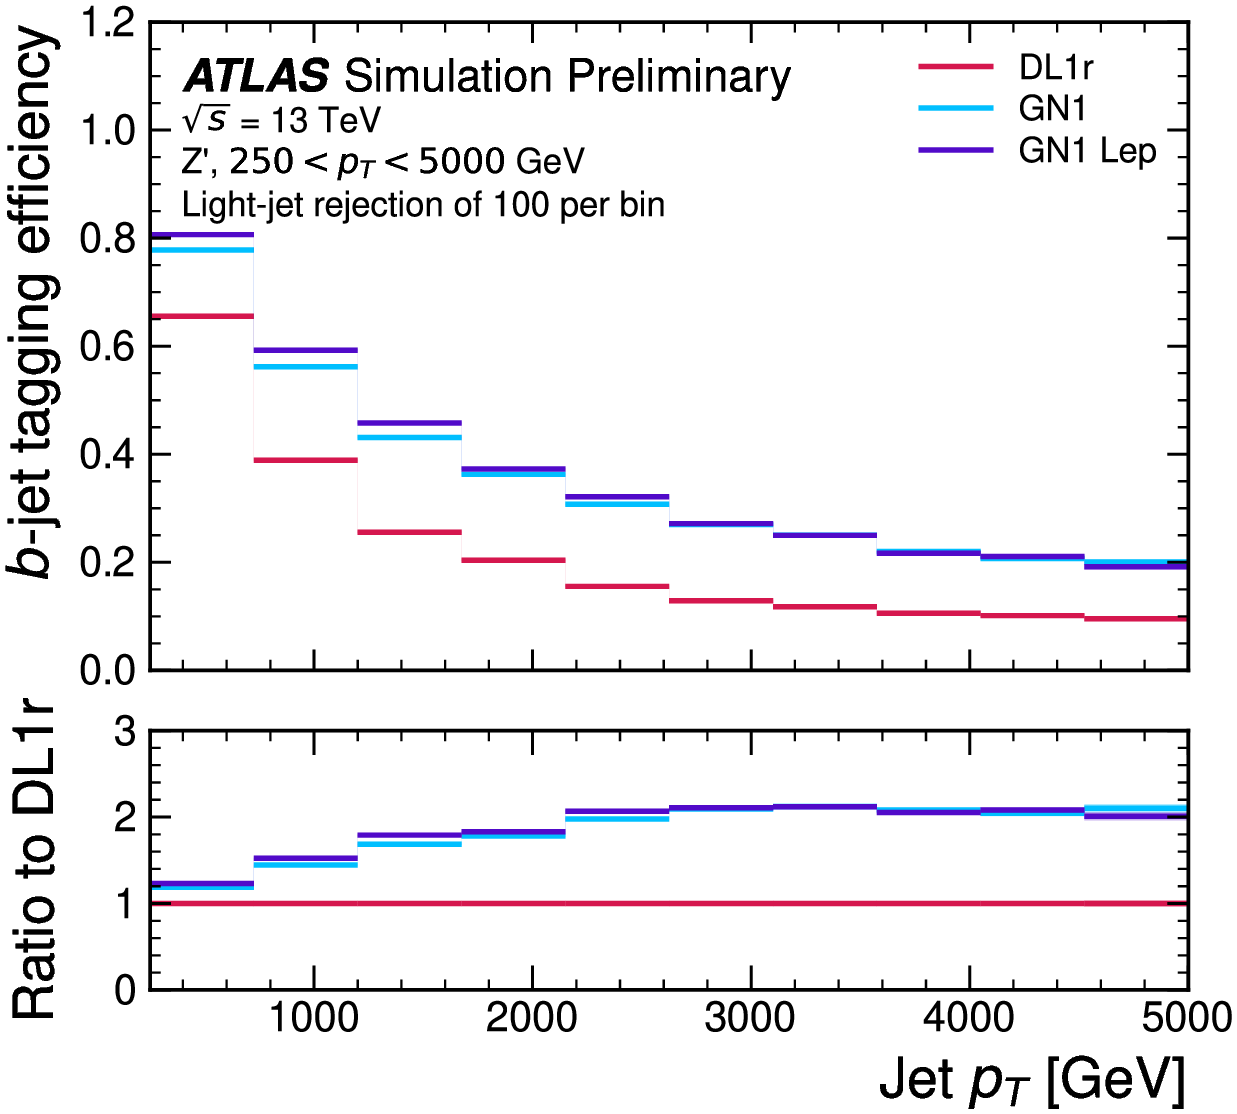
\includegraphics[width=0.45\textwidth]{Images/FTAG/GN/GN1/eff/ptzpb.png}
  \caption{Comparing the GN1 and DL1r $b$-tagging efficiency as a function of jet $p_T$ at a fixed 100 light-jet rejection in each bin on the $t\bar{t}$ (left) and $Z'$ (right) test samples, from \cite{ATL-PHYS-PUB-2022-027}. Models compared are DL1r in dashed lines and GN1 in continuous line. The flavour fraction is set at $f^b_c = 0.018$ for DL1r and 0.05 for GN1 and GN1 Lep.}
  \label{fig:GN1ptb}
\end{figure} 

To conclude this chapter on \gls{gn1}, the importance of the auxiliary tasks is discussed by presenting ablations studies removing them iteratively from the full \gls{gn1} model. For this purpose, three variants of \gls{gn1} were trained equivalently to the full \gls{gn1} but without:
\begin{itemize}
  \item any auxiliary objectives, leading to a model label ``GN1 No Aux'' only optimising the jet classification objective,
  \item the vertexing objective but not the track classification one, for the model labelled ``GN1 Vert'',
  \item the track classification objective without vertex, referred to as ``GN1 TC''.
\end{itemize}
Figure \ref{fig:GN1ablb} displays the \gls{roc} curves of theses modified model with respect to the previously introduced \gls{dl1r} and the full \gls{gn1}. Removing either or any of the auxiliary objectives is seen to have a large impact on performance. The \gls{gn1} No Aux model is effectively similar to a \gls{dl1d} model, having similar performance gains with respect to \gls{dl1r}. Remarkably, this performance is obtained from a single network processing tracks without any of the sub-tagger nor methods used by the \gls{dl1} family, effectively underlying the powerful representation power of \gls{gat}. Adding either of the auxiliary task has the same beneficial impact on performance, as GN1 TC and GN1 Vert performs similarly and each is enough to outmatch \gls{dl1r}. The real gain is obtained by adding both auxiliary taks, which further boosts the effectiveness of the model. 

\begin{figure}[h!]
  \centering
  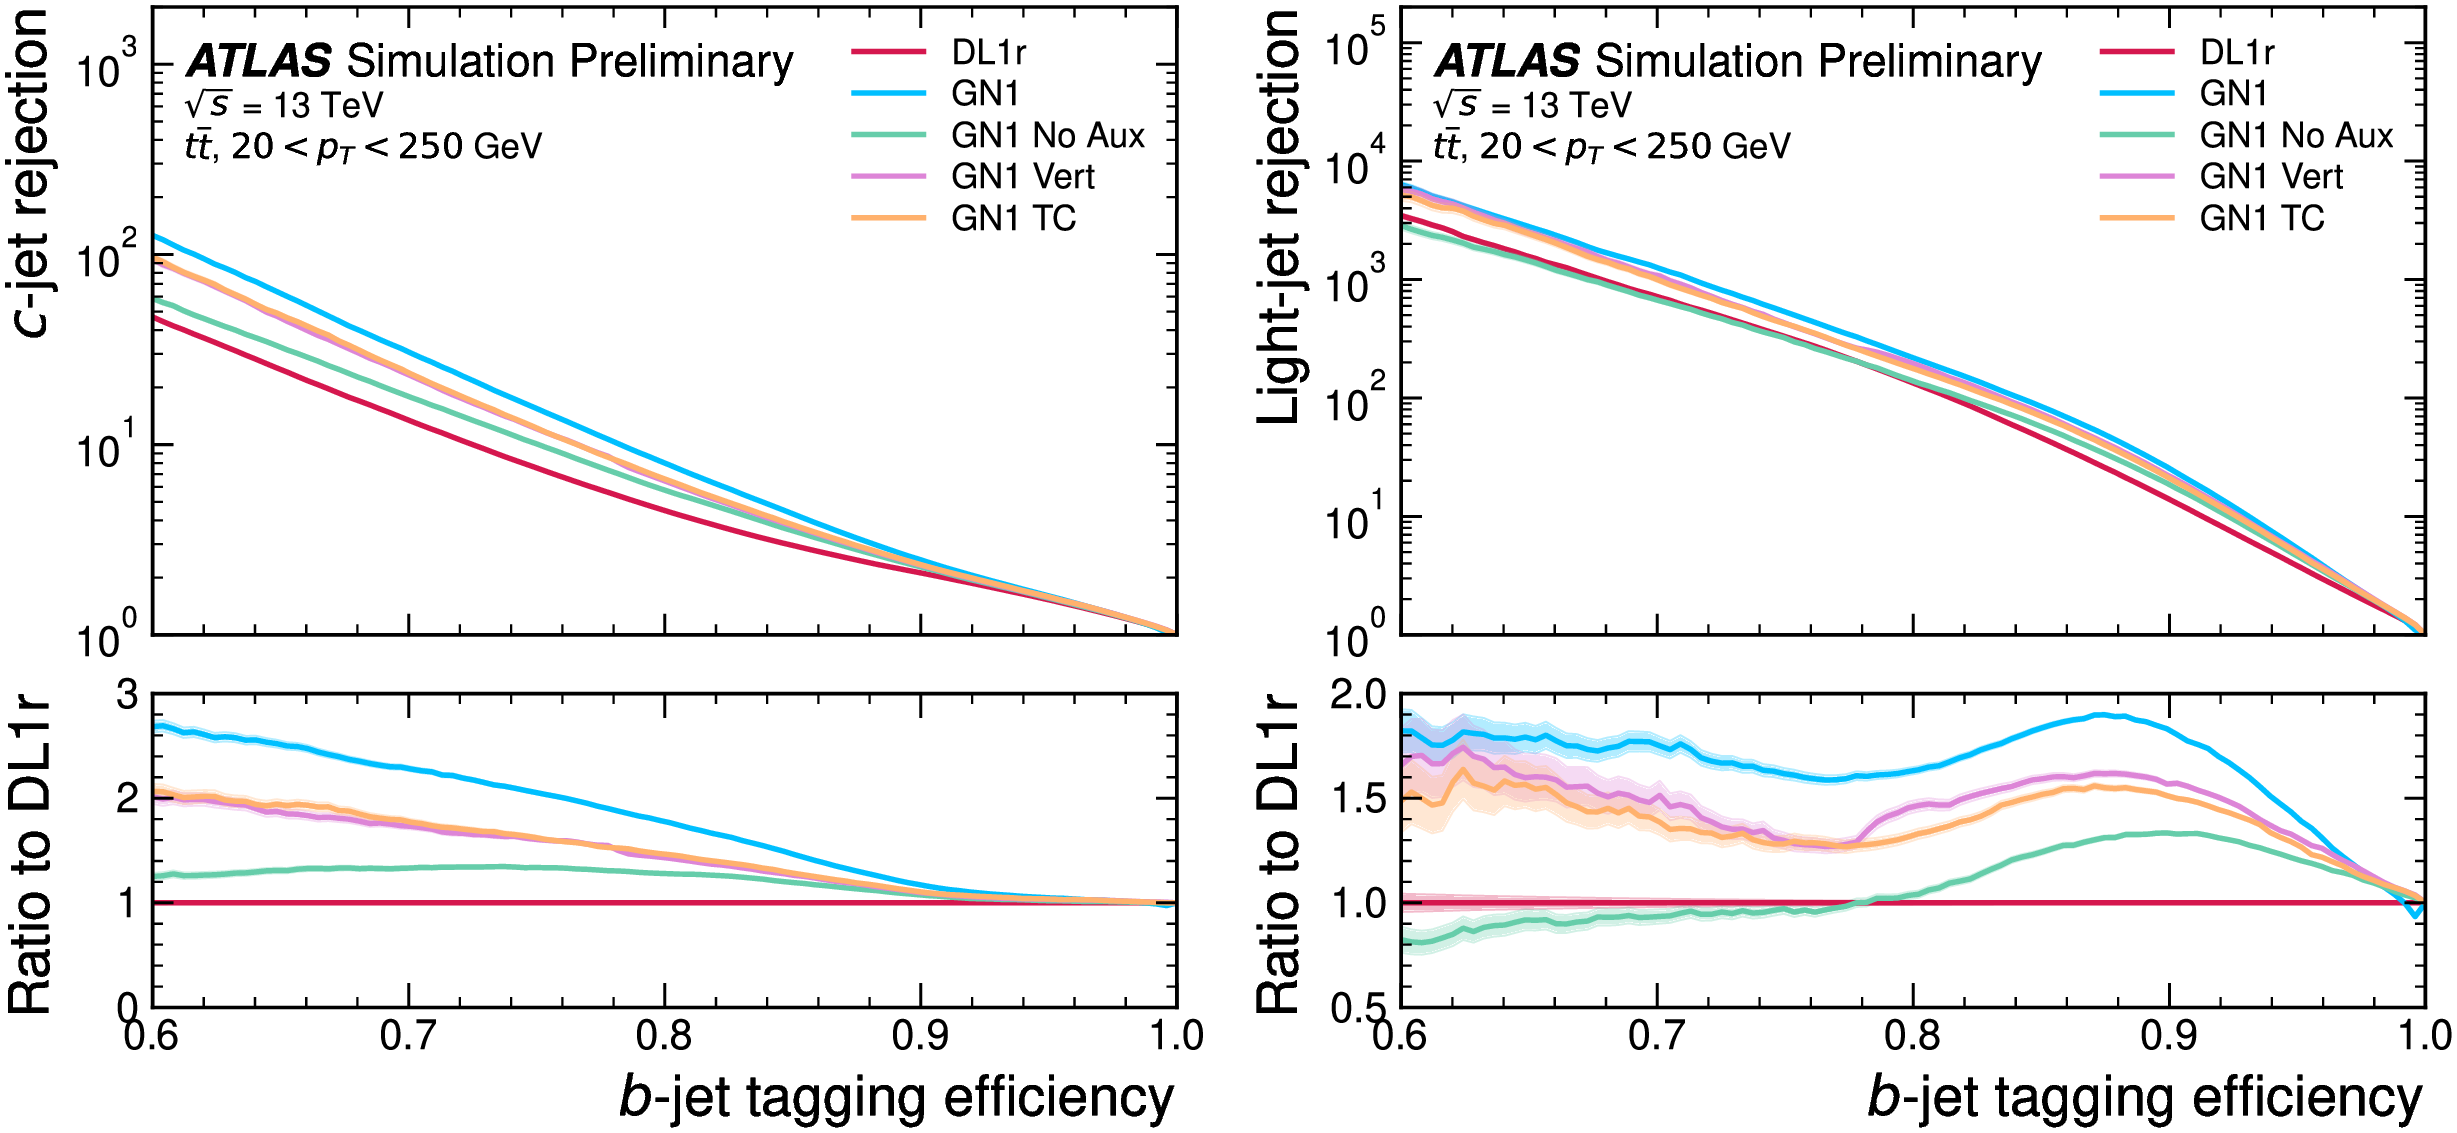
\includegraphics[width=0.98\textwidth]{Images/FTAG/GN/GN1/ablations/ttb.png}
  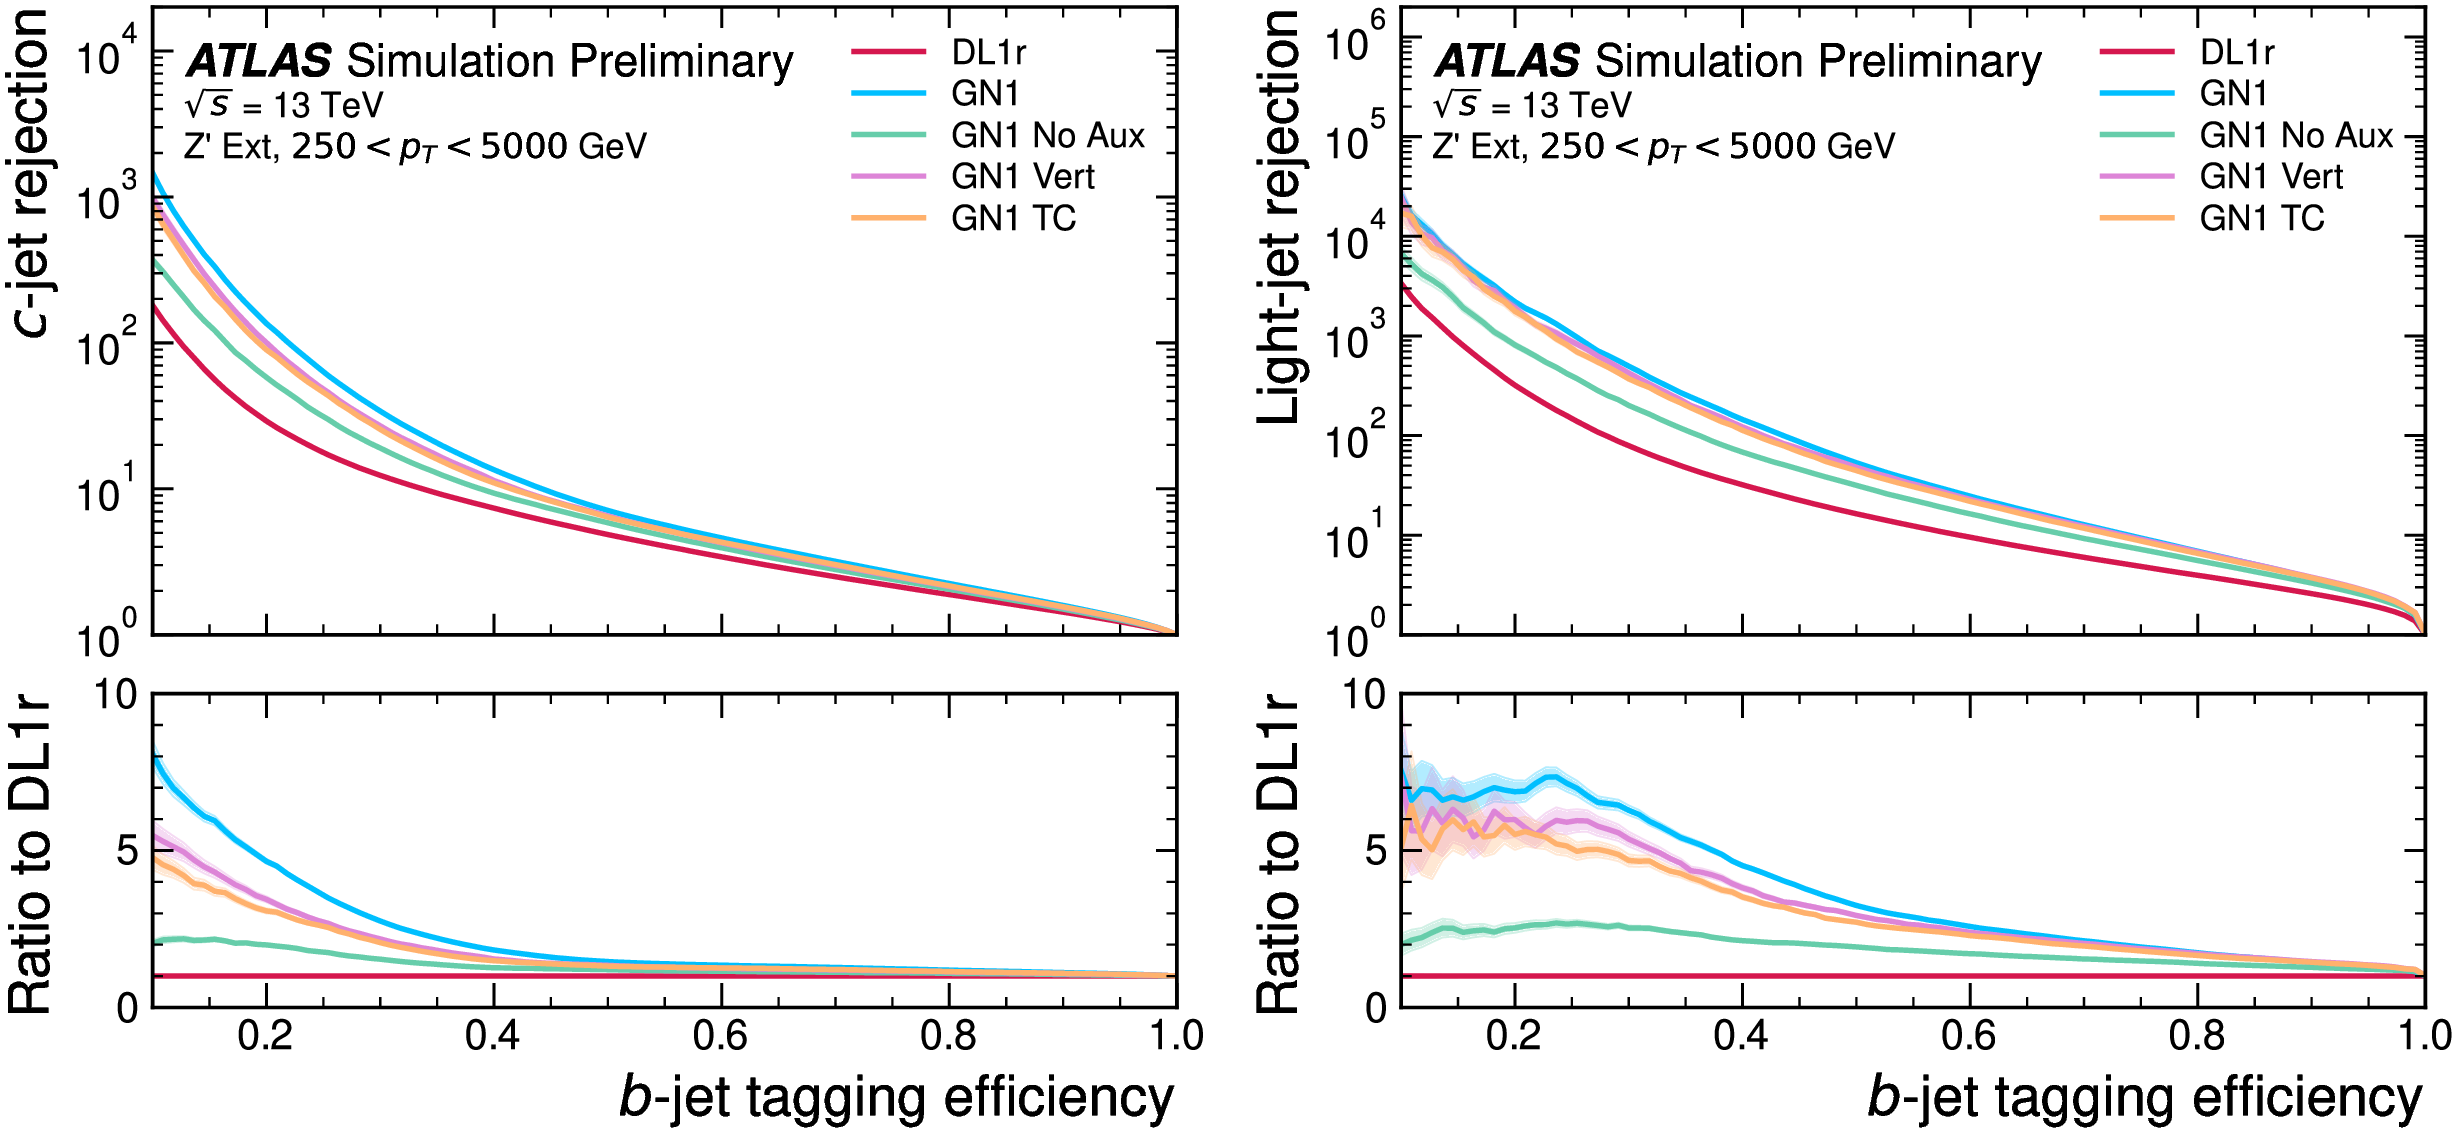
\includegraphics[width=0.98\textwidth]{Images/FTAG/GN/GN1/ablations/zpb.png}
  \caption{ROC curves tracing the $b$-tagging efficiency versus the $c$-rejection (left) and light-rejection (right) for the $t\bar{t}$ (top) and $Z'$ (bottom) test samples, from \cite{ATL-PHYS-PUB-2022-027}. Models compared are DL1r in red, GN1 in blue, and versions of GN1 with missing auxiliary tasks. GN1 No Aux in green has none of the auxiliary, GN1 Vert in purple only the vertexing task, and GN1 TC in orange only the track classification. The flavour fraction is set at $f^b_c = 0.018$ for DL1r and 0.05 for GN1. The binomial error bands are shown as shaded regions.}
  \label{fig:GN1ablb}
\end{figure} 

So far, the performance of \gls{gn1} on the primary objective of jet flavour classification has been discussed. The performance on the auxiliary objectives was not initially intended to be leveraged on real data but only to distill information for the primary goal. The track-pairs vertexing performance can be assessed by leveraging the information to perform track finding: grouping sets of tracks that are found to share a vertex with one another into a single vertex. The result is compared to the truth vertex label available in the simulations. Vertices identified by \gls{gn1} as containing tracks coming from a $b$-hadron decay are grouped together, and the same procedure is applied to the truth information. To measure performance, the reconstructed and true vertices are compared as well as the number of tracks correctly assigned. A vertex is correctly identified when it contains at least 65\% of the correct tracks with a purity of at least 50\%. The comparison is only carried out for reconstructed tracks, meaning a 100\% \gls{gn1} efficiency corresponds to correctly identify all possible secondary vertices within the limit of the track reconstruction efficiency. An inclusive reconstruction efficiency in $b$-jets of $\sim$80\% is measured for \gls{gn1}, effectively proving that the model is able to identify $b$-hadron decay vertices. An important caveat is the current restriction is only on finding such vertices, not on a reconstructing them. In order to implement a fully-fledged secondary vertex fitter as an auxiliary objective, the fitting of the vertex must be produced by a differentiable algorithm to allow for backpropagation. This is a promising area of research, given the global interest in accessing this much-used \gls{sv} information. Recent work has been carried out to introduce this task using the differentiable single vertex fitting algorithm of Ref. \cite{smith2023differentiable}. \\

\begin{figure}[h!]
  \centering
  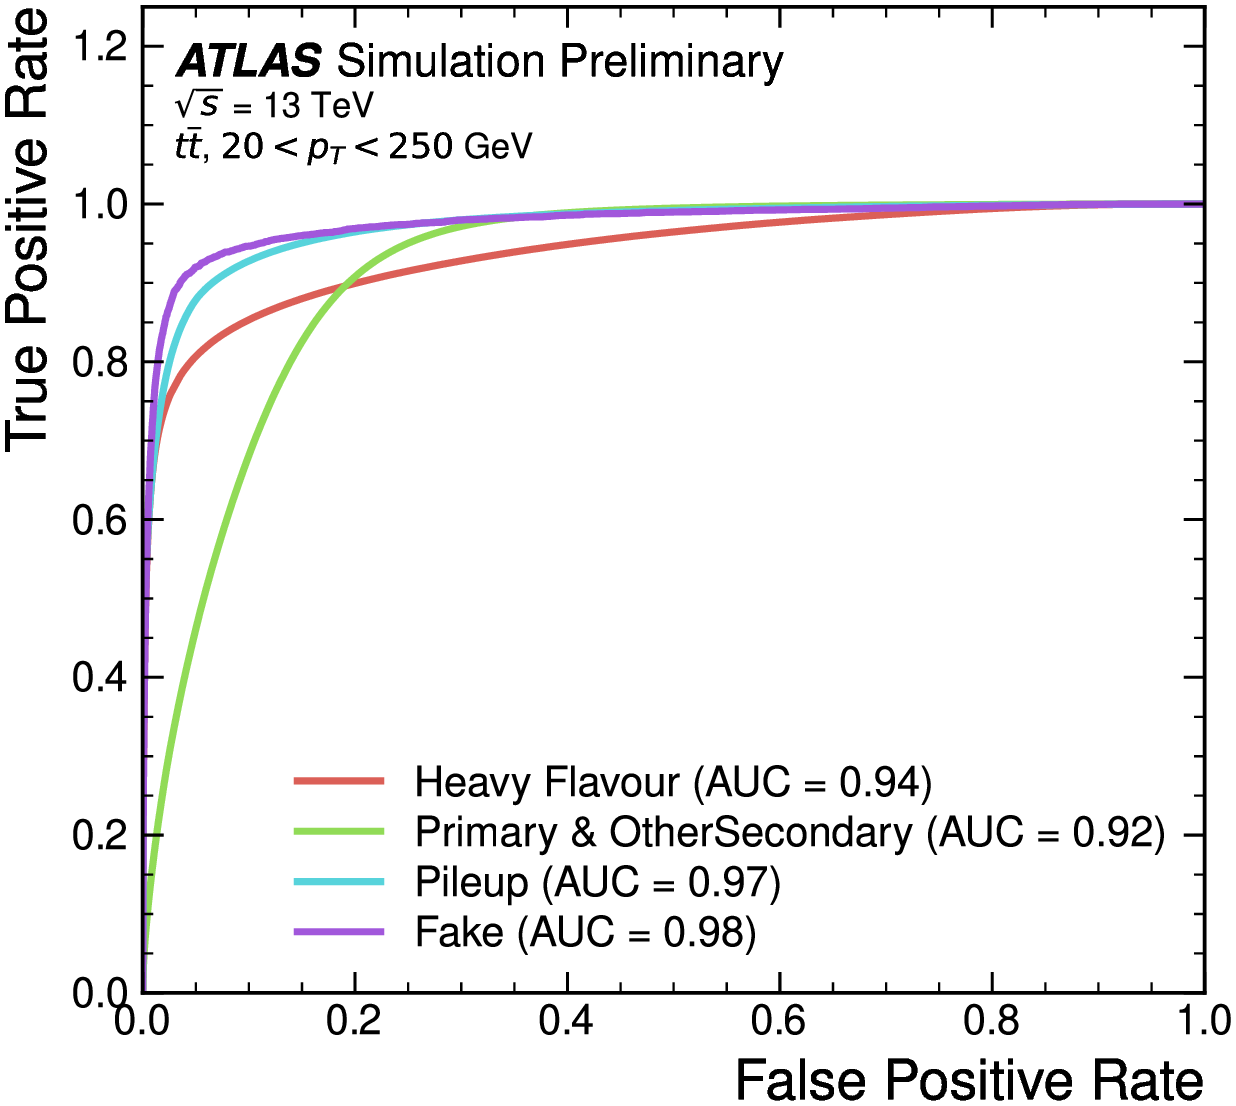
\includegraphics[width=0.48\textwidth]{Images/FTAG/GN/GN1/ablations/ttroc.png}
  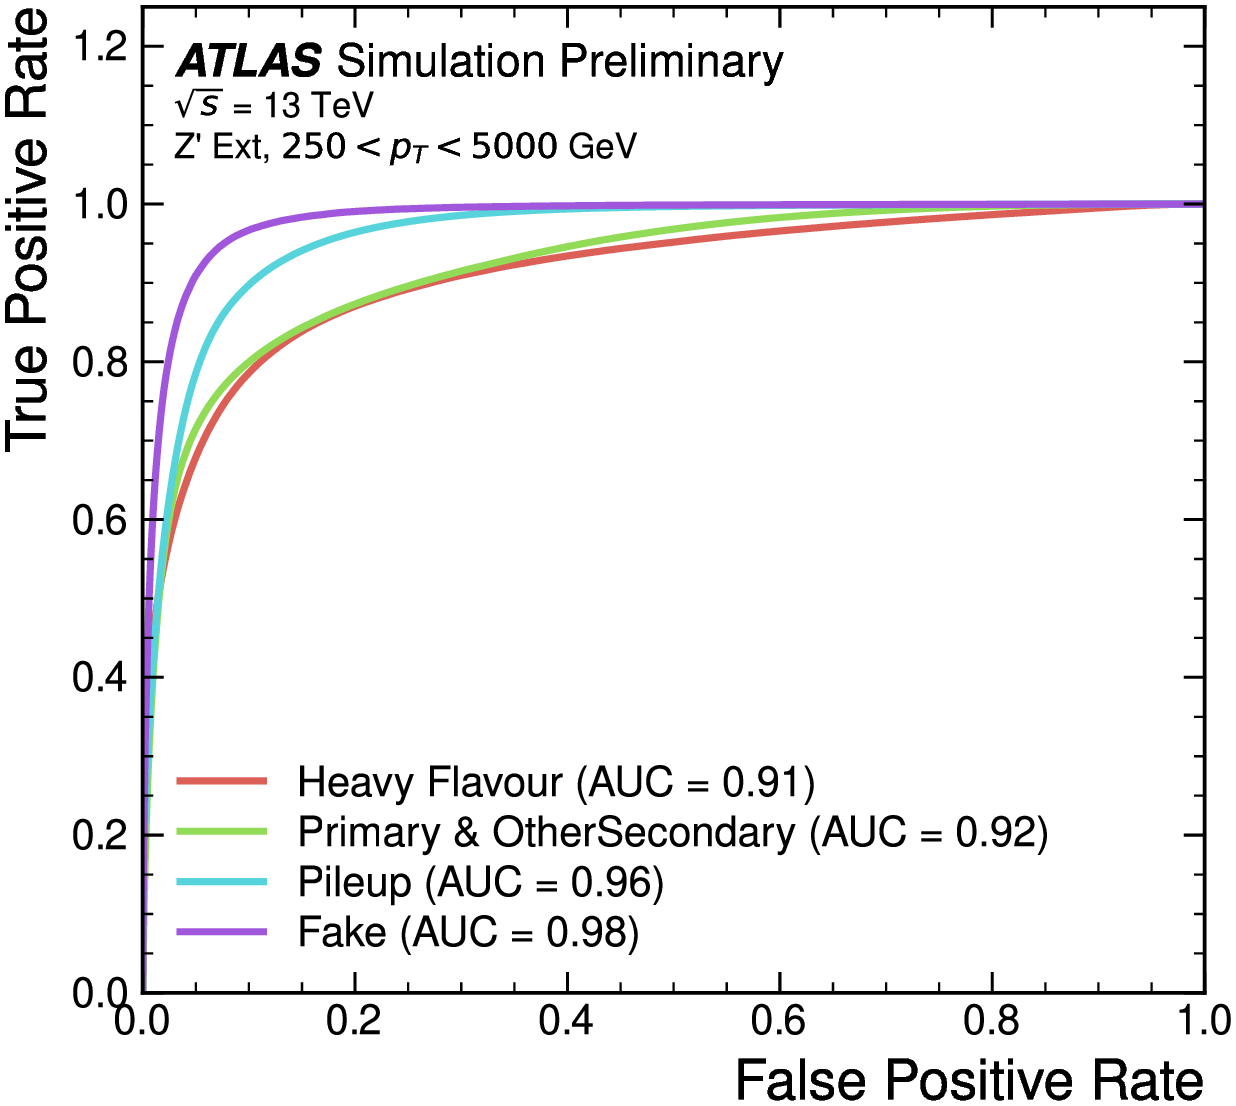
\includegraphics[width=0.48\textwidth]{Images/FTAG/GN/GN1/ablations/zproc.png}
  \caption{ROC curves tracing the false positive rate versus the true positive rate of the truth origin classification on the $t\bar{t}$ (left) and $Z'$ (right) test samples, from \cite{ATL-PHYS-PUB-2022-027}. Heavy Flavour is a weighted combination of the FromB, FromBC, and FromC by their relative abundance.}
  \label{fig:GN1trackperf}
\end{figure} 

Concerning the track origin classification performance, Figure \ref{fig:GN1trackperf} presents the traditional \gls{roc} curves, comparing the false positive rate (tracks wrongly assigned a label) versus the true positive rate (correctly assigned the label), for the different track origin classes of Table \ref{tab:gnTrackOrigin}. Some classes are combined with weights dictated by the class relative abundance: this is the case of the FromB, FromBC, and FromC classes that are combined as Heavy Flavour, and the Primary and OtherSecondary labels. The \gls{auc} of the \gls{roc} of all groups is above 90\%, indicating good classification performance. The most challenging categories are the Heavy Flavour, Primary, and OtherSecondary tracks, while the Fake and Pileup tracks were most easily identified. The global mean (weighted) \gls{auc} was of 92\% (95\%) on $t\bar{t}$ and 94\% (96\%) on $Z'$ \cite{ATL-PHYS-PUB-2022-027}. This performance is in line with a physics-based intuition, and the $p_T$ effect can be noted by the reduction in \gls{auc} for the Heavy Flavour tracks on the $Z'$ sample. \\

\gls{gn1} proved to be an exciting direction of development for flavour tagging at ATLAS. It showed clear benefit from the previous mentality of building network by combining several algorithms and methods with physics meaning. Embrassing modern advanced machine learning, it relies on a single network built around an advanced graph attention network. While the functioning of the model is less intepretable than the previous \gls{dl1} family of tagger, expert knowledge is still instilled in the model thanks to the multitask paradigm. Building on from this success, an upgrade architecture was developped to accelerate the speed of training and continue pushing the performance of the method ever higher: \gls{gn2}.

\subsection{GN2: a Transformer Encoder for Flavour Tagging}\label{chap-GN2}
\gls{gn2} is not a radical change on the architecture of \gls{gn1}. Rather, it is a fine-tuned modified model aiming to reproduce the same conceptual processing chain as \gls{gn1}, only with an easier to train and simpler to scale design. The main modifications with respect to \gls{gn1} is the replacement of the computationally complex and expensive graph attention operator by a now famous architecture in machine learning: the transformer \cite{NIPS_transformerPaper}. As described in Chapter \ref{sec:transformer}, the transformer is a remarkably effective and expressive design, both able to extract fine-grained correlations between ordered and unordered tokens in a sequence through the mechanism of attention and to scale to very large network size without suffering from overtraining. By design, transformers combine rich attention computing and regularisation inducing steps which let such network scale significantly in number of parameters while guaranteeing effective parallelisable training on \gls{gpu} hardware. \\

In the case of \gls{gn2}, given the design only requires building a global represenation of the sets of tracks composing a jet, only the encoder part introduced in Ref \cite{NIPS_transformerPaper} and modified in Ref \cite{shleifer2021normformer} is deployed instead of the \gls{gnn} component of Figure \ref{fig:ftagArchi}. A dense summary of the modifications applied when moving from \gls{gn1} to \gls{gn2} is presented in Table \ref{tab:gn2compGN1}. The reference to \gls{gn1} corresponds to the last version of the model that was developped which explains some small modifications with the model described in the previous chapter. Similarly, the \gls{gn2} model described here corresponds to the first publically released model, and this generation is also being refined and improved at the time of writing this thesis. 

\begin{table}[h]
  \begin{center}
      \begin{tabular}{c|c|c|c} 
      	 \hline \hline
          Modification & Parameter & GN1 & GN2 \\ \hline
          Hyperparameter  & Trainable parameters & 0.8M & 1.5M \\ 
          Hyperparameter  & Learning rate & Fixed 1e-3 & One-cycle scheduler\\ 
          Hyperparameter  & Core unit layers & 3 & 6 \\ 
          Hyperparameter  & Attention heads & 2 & 8 \\ 
          Hyperparameter  & Embedding dimension & 128 & 192 \\ \hline
          Architecture    & Attention Type & \gls{gat}v2 & Scaled dot product \\ 
          Architecture    & Dense update & No & Yes (dim 256) \\ 
          Architecture    & Separate value projection & No & Yes \\ 
          Architecture    & LayerNorm + Dropout & No & Yes \\ \hline
          Inputs          & Number of training jets & 30M & 192M  \\ \hline \hline
      \end{tabular}
    \caption{Main modifications between the last generation of GN1 and the first generation of GN2, taken from \cite{ATL-PLOT-FTAG-2023-01}.}
    \label{tab:gn2compGN1}
  \end{center}
\end{table}

Some significant changes adopted for \gls{gn2} are a learning rate scheduler, a larger embedding space dimension giving a wider and deeper - thanks to the doubling of the number of layers - of the core units (the \gls{gnn} for \gls{gn1} and the transformer for \gls{gn2}), and the introduction of regularising effects from layer normalisation and dropout \cite{ba2016layer}. The learning rate scheduler is based on the one-cycle scheduler of Ref \cite{smith2018disciplined}, with some important  parameters described in Table \ref{tab:onecyclescheduler}. This scheduler speeds up the training by initially growing the learning rate to large values, corresponding to large steps in the parameters' optimisation landscape, before annealing progressively the learning rate to small values, helping to converge on a specific minimum \cite{smith2018superconvergence}. The attention implemented in the transformer allows similar physics performance at a reduced memory footprint and training time \cite{duperrin2023flavour}. The improved computational performance of \gls{gn2} made it possible to scale the network up in terms of number of parameters, \gls{gn2} having roughly twice as many parameters as \gls{gn1}, but also in terms of training dataset. \gls{gn2} can indeed be trained on roughly $\times 6$ more jets than \gls{gn1} with the same computing resources. The datasets for the \gls{gn2} training presented here was derived in the same fashions as those of \gls{dl1d} and \gls{gn1}, using importance sampling to fully utilise the $b$- and light-jets statistics. 

\begin{table}[h]
  \begin{center}
      \begin{tabular}{c|c} 
      	 \hline \hline
          Parameter   & Description \\ \hline
          LR initial  & Initial value of the learning rate   \\ 
          LR maximal  & Maximal value of the learning rate, reached at the end of warm up   \\ 
          LR final    & Value of the learning rate reached at peak epoch    \\ 
          Warm Up     & Period covering the increase from initial to maximal   \\ 
          Peak epoch  & Epoch at which LR maximal should be reached   \\ \hline \hline
      \end{tabular}
    \caption{The five parameters of the one-cycle scheduler.}
    \label{tab:onecyclescheduler}
  \end{center}
\end{table}

The attention mechanism in the transformer is subtly different from the \gls{gat}, and corresponds to the multihead self-attention process described in Chapter \ref{sec:transformer}. The nodes are updated in a two steps approach: first attention is computed and applied, then a dense layer updates the set of nodes. In more details, the transformer implements the following update on the set of nodes $h_i \in \mathcal{N}$ defining the fully connected graph $G(\mathcal{N})$:
\begin{enumerate}
  \item Layer normalisation is applied to the input set of nodes $\mathcal{N}$
  \item For each attention head, three individual mapping represented by layers $W_q$, $W_k$, and $W_v$ map each node $h_i \in \mathcal{N}$ to three independent representations $W_qh_i$, $W_kh_i$, and $W_vh_i$.
  \item For each node $h_i \in \mathcal{N}$, edge scores are computed with all nodes $h_j$ using the scaled dot product attention \[e\left(h_i, h_j\right) = \frac{W_q h_i\, . \, W_k h_j}{\sqrt{s}},\] where the $s$ parameter representing the scaling weight is typically taken to be the dimension of matrix $W_k$. 
  \item The edge scores are turned into attention scores for node $i$, by taking the softmax over all nodes: \[a_{i, j} = \textrm{softmax}_j\left(e(h_i, h_j) \right) \]
  \item Each node $h_i \in \mathcal{N}$ is updated into a node $h_i' \in \mathcal{N}'$ as: \[h_i' = \sum_j a_{i, j} \,.\, W_v h_j\]
  \item Using a skip connexion, the updated nodes $\mathcal{N}'$ are added the original nodes $\mathcal{N}$ values. 
  \item Layer normalisation is applied to the updated nodes $\mathcal{N}'$.
  \item The updated nodes are passed through a \gls{dnn}.
  \item The output of the \gls{dnn} is summed to the updated nodes by a skip connexion, given the final updated set of nodes $\mathcal{N}'$.
\end{enumerate}

The \gls{gn2} model presented here combines 6 such transformer layers with 8 attention heads in total. A comparison of the global performance of this \gls{gn2} model to the \gls{dl1r}, \gls{dl1d}, and \gls{gn1} models is displayed in the $b$-tagging \gls{roc} curves of Figures \ref{fig:GN2rocb}. For this comparison, the \gls{gn2} and \gls{dl1d} models have been retrained on the same datasets, with the \gls{dl1r} and \gls{gn1} models equivalent to those presented in the previous Chapter \ref{chap-GN1}. \gls{gn2} delivers yet another significant boost to performance, drasticaly surpassing the \gls{gn1} rejections at all efficiencies considered. The largest improvement is again obtained at lower $b$-jet efficiencies. Compared to \gls{gn1}, \gls{gn2} delivers $\times 1.5$ ($\times 1.7$) the $c$-rejection (light-rejection) on $t\bar{t}$ at the 70\% $b$-tagging \gls{wp} and $\times 1$ ($\times 1.7$) on $Z'$ at 30\% \gls{wp}. With respect to \gls{dl1d}, the gains in $c$-rejection (light-rejection) are respectively close to $\times 3$ ($\times 2$) for $t\bar{t}$ and $\times 3$ ($\times 4$) on $Z'$. The $c$-rejection on $Z'$ of the \gls{gnn} models is essentially equivalent, although the significantly improved light-rejection of \gls{gn2} indicates its $c$-rejection can be boosted by further increasing its flavour fraction $f^b_c$ above 0.1. \\

Turning to $c$-tagging, as displayed in Figure \ref{fig:GN2rocc}, a similar large performance gained is obtained by the new \gls{gnn} family over the \gls{dl1} one, both in terms of $b$- and light-rejection. \gls{gn2} again introduces a large improvement on top of \gls{gn1}, although their $b$-rejection performance is equivalent on $Z'$. The gains from \gls{gn2} with respect to \gls{gn1} are of a factor $\times 1.3$ ($\times 1.3$) for $b$-rejection (light-rejection) on $t\bar{t}$ at the 30\% \gls{wp}, while they are $\times 1$ ($\times 1.2$) on $Z'$. The comparison to \gls{dl1d} is of $\times 1.9$ ($\times 2.1$) on $t\bar{t}$ and $\times 1.3$ ($\times 1.8$) on $Z'$ at the same \gls{wp}.

\begin{center}
  \begin{figure}[h!]
  \centerline{
  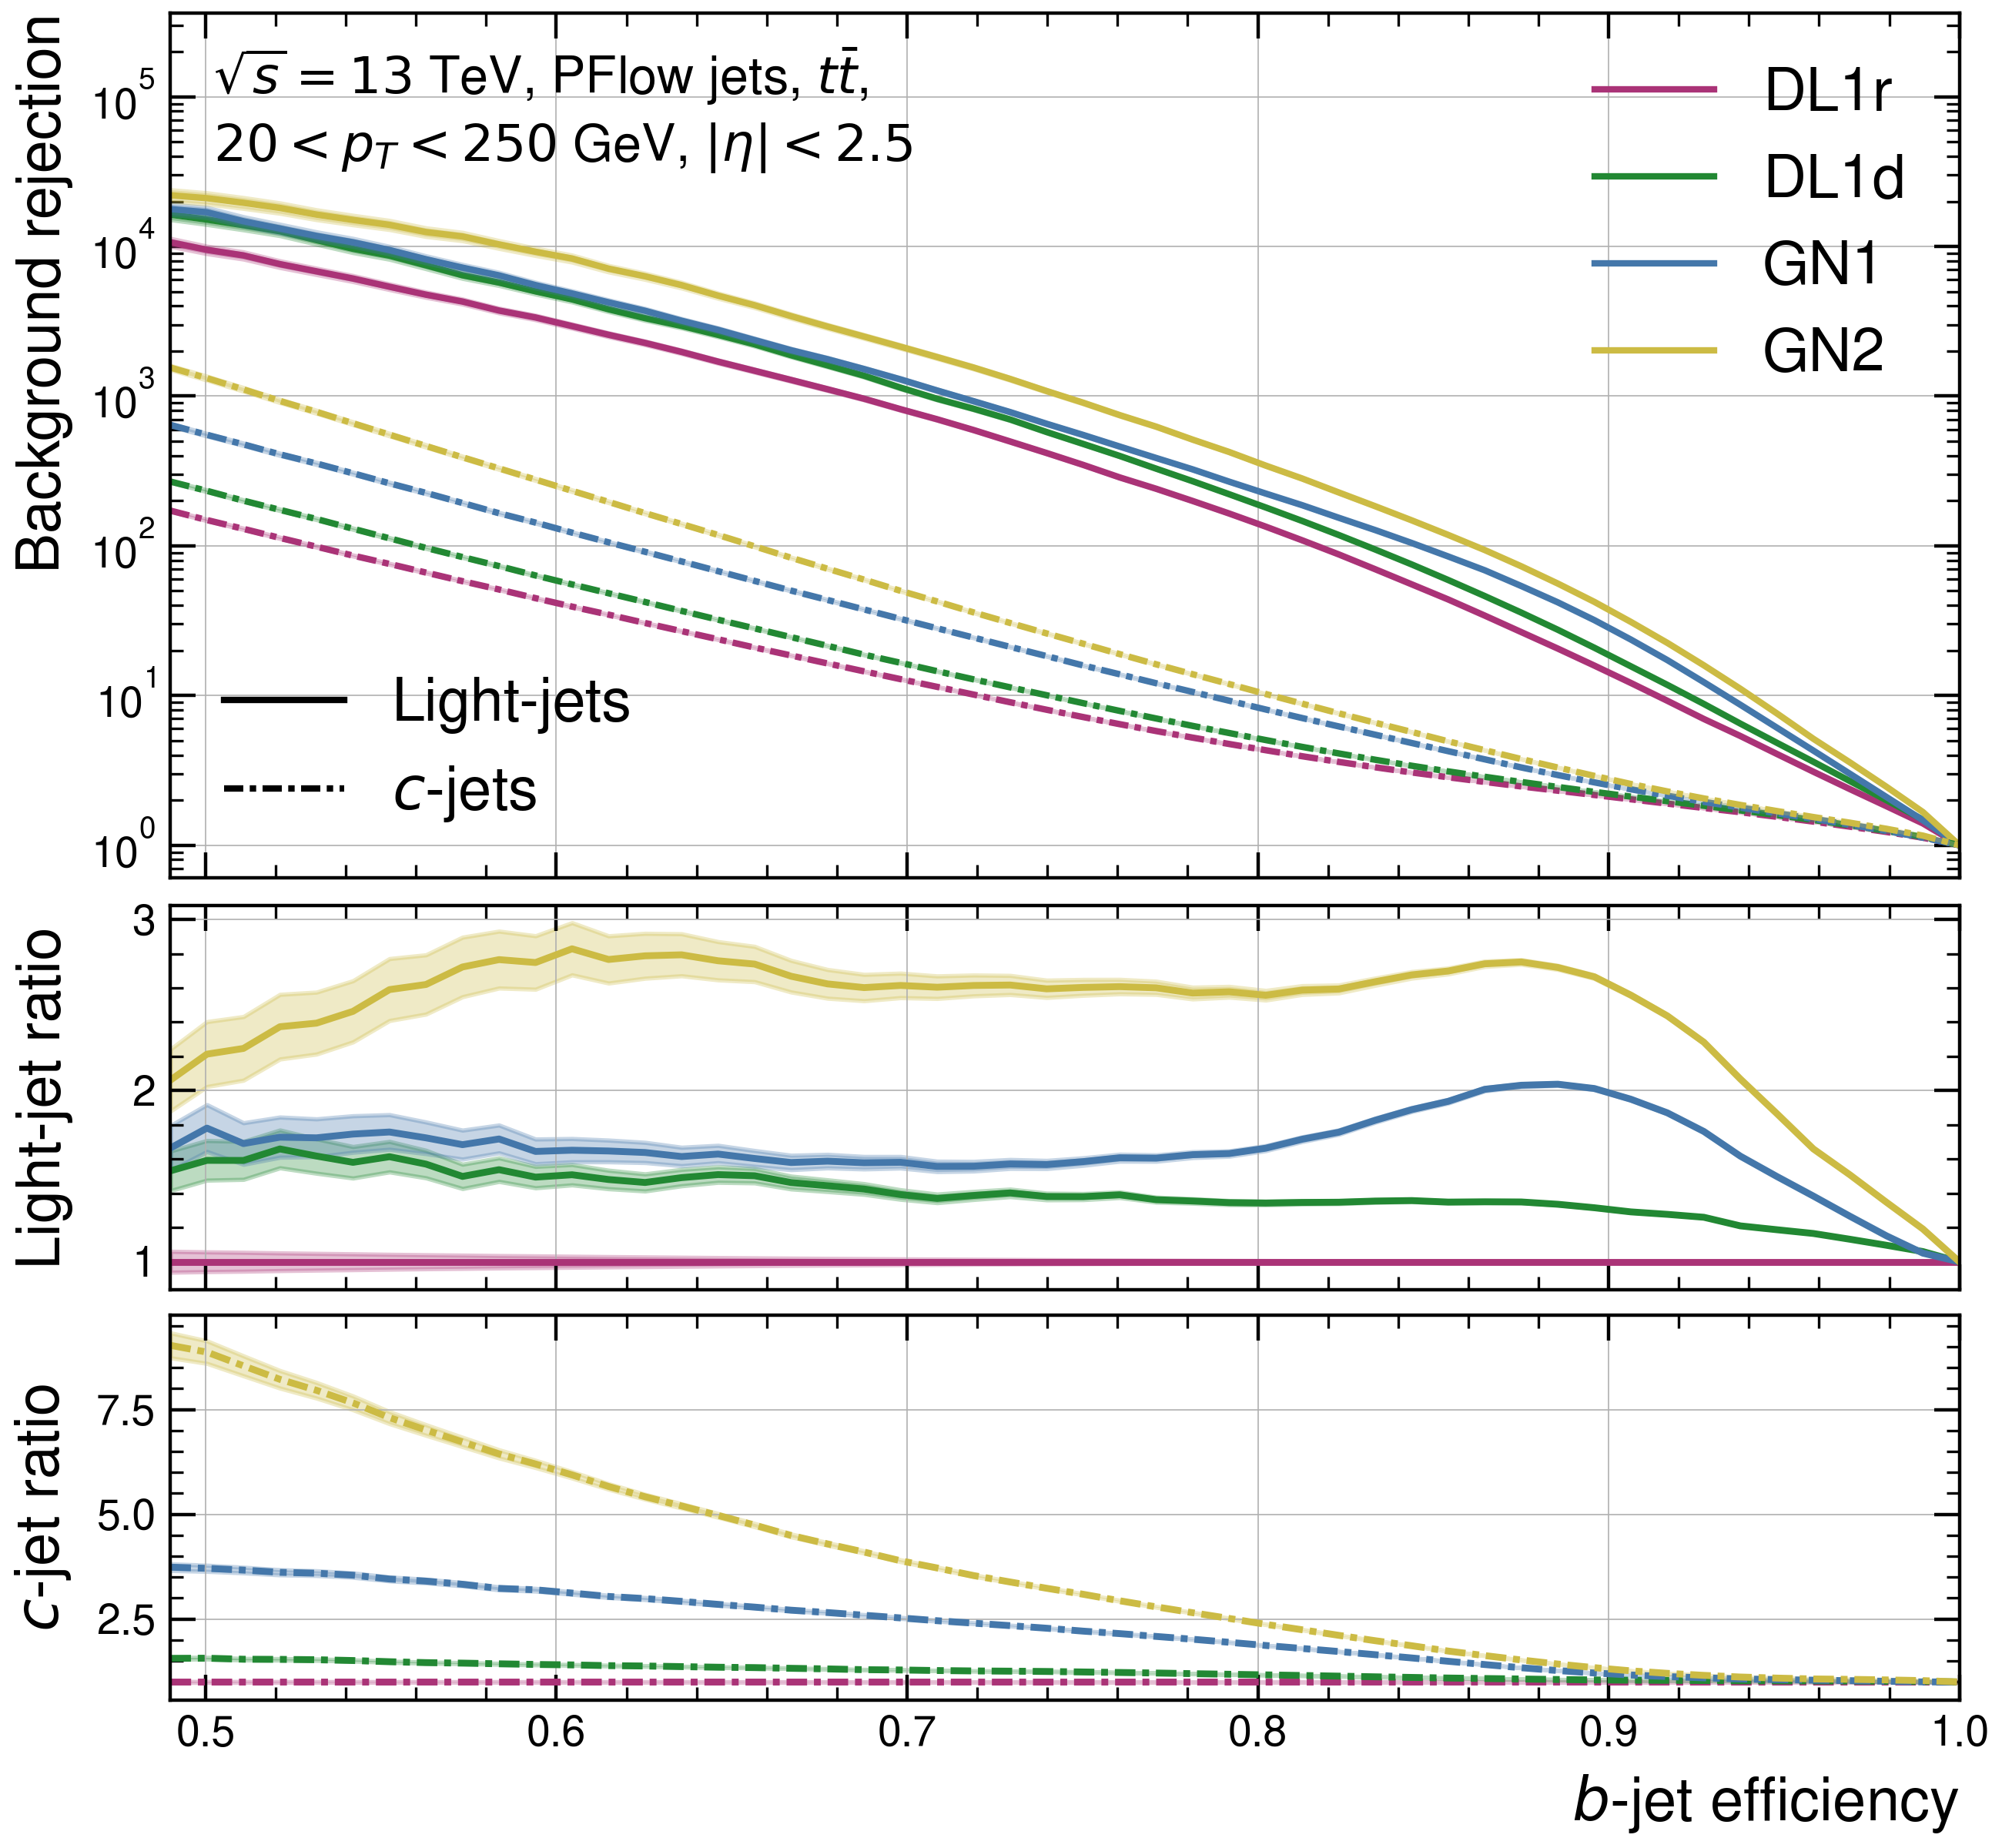
\includegraphics[width=0.50\textwidth]{Images/FTAG/GN/GN2/rocs/roc_ttbar.png}
  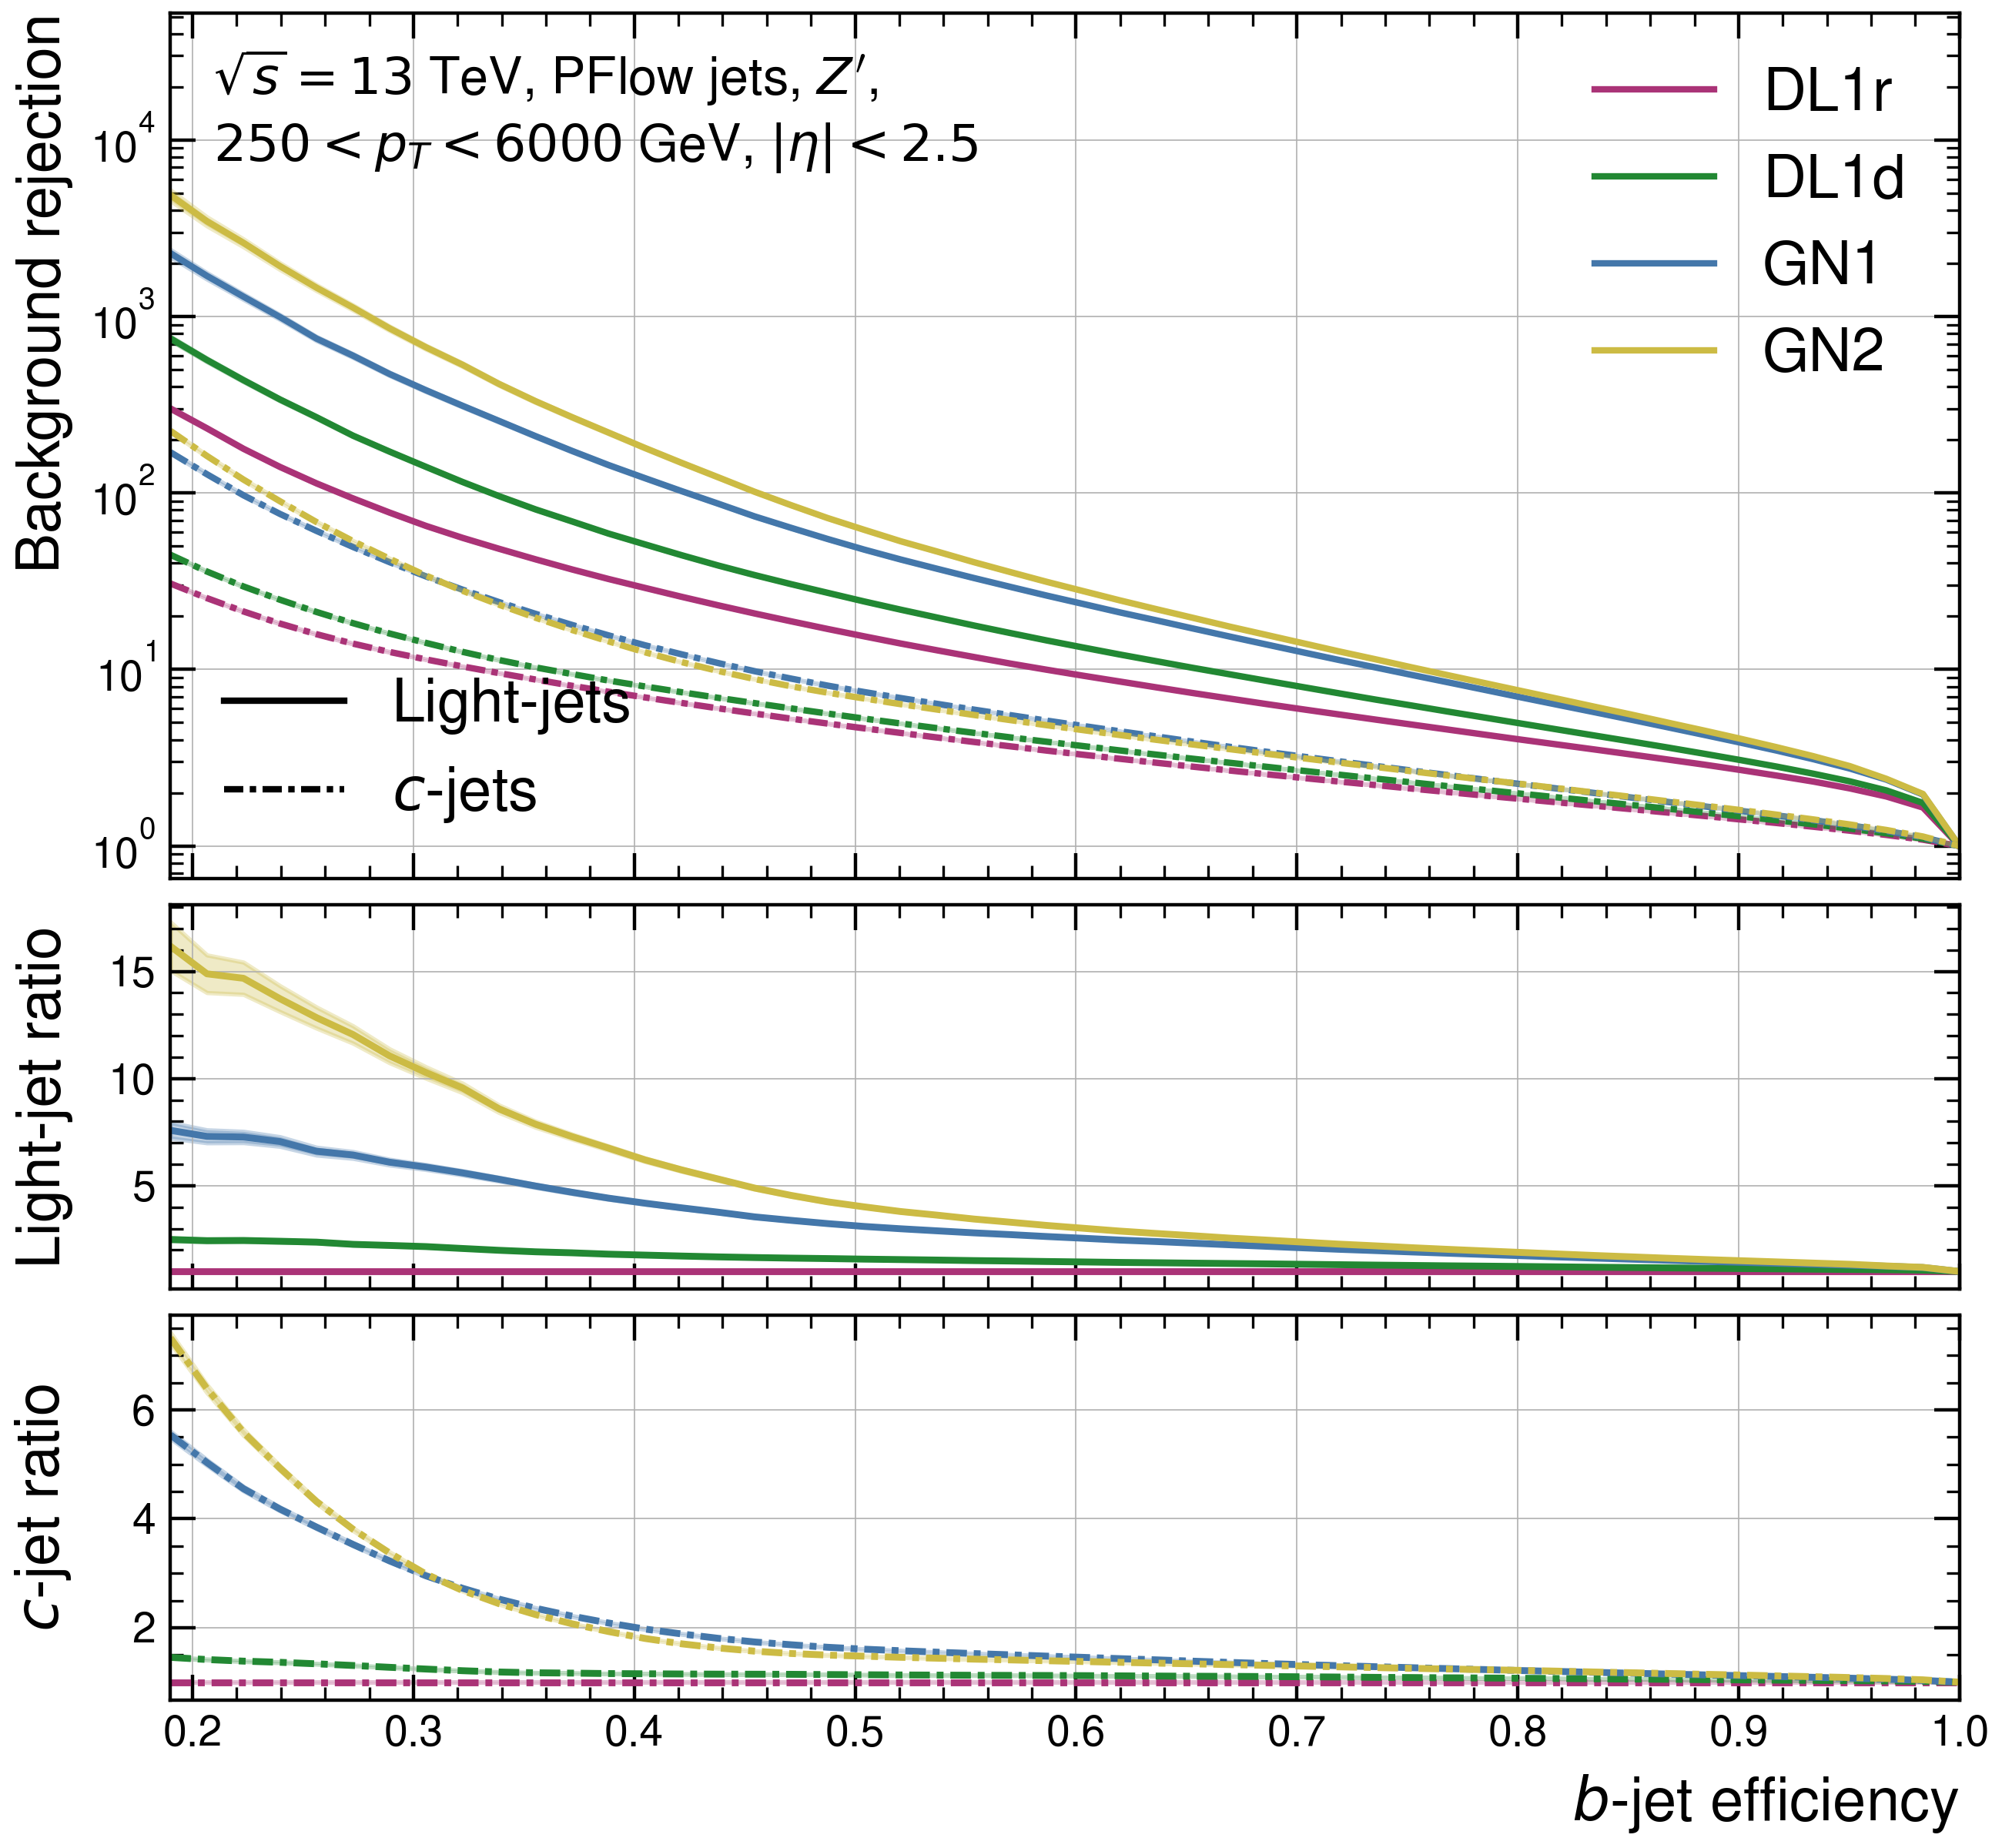
\includegraphics[width=0.50\textwidth]{Images/FTAG/GN/GN2/rocs/roc_zp.png}
  }
  \caption{The $c$- and light-rejections as a function of the $b$-jet tagging efficiency in the $t\bar{t}$ with $20 < p_T < 250$ GeV (left) and $Z'$ with $250 < p_T < 6000$ GeV (right) test samples. Models compared are DL1r in purple, DL1d in green, GN1 in blue, and GN2 in yellow. The bottom plots show the ratio with respect to the DL1d performance. Flavour fractions are set at $f^b_c = 0.018$ for DL1r and DL1d, 0.05 for GN1, and 0.1 for GN2. Shaded regions represent the binominal error band.}
  \label{fig:GN2rocb}
  \bigskip
  \centerline{
  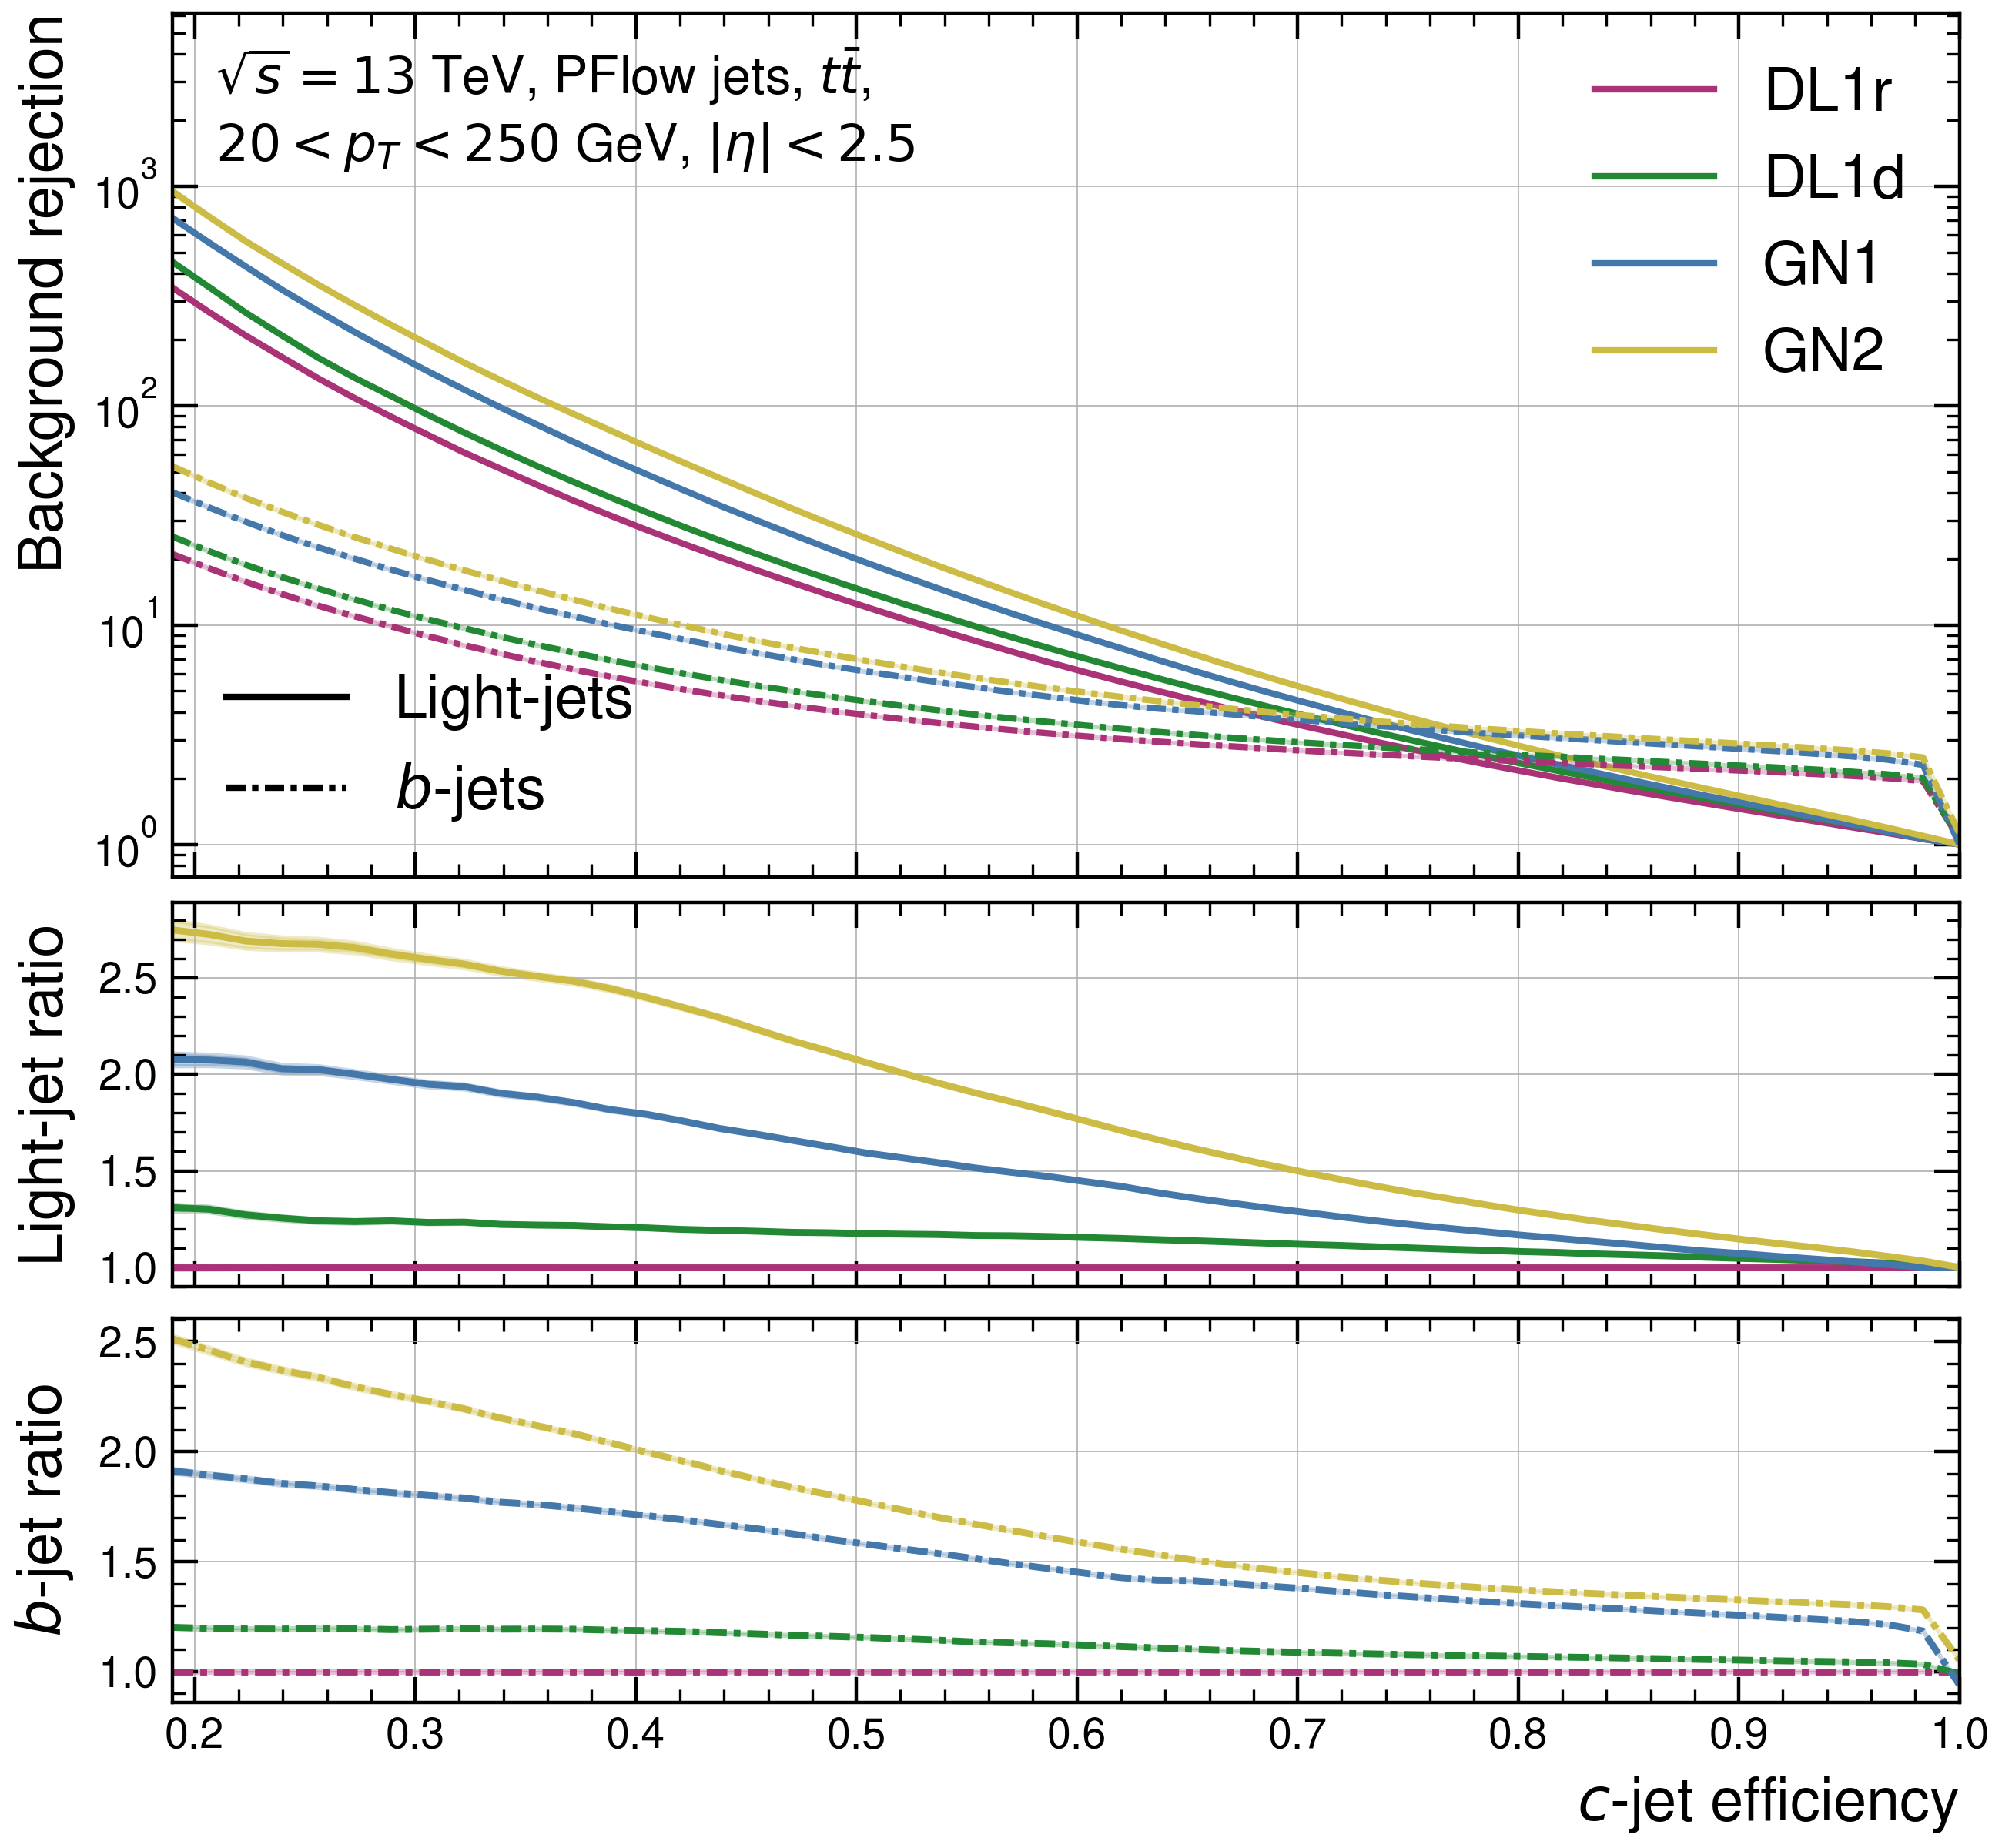
\includegraphics[width=0.50\textwidth]{Images/FTAG/GN/GN2/rocs/roc_ttbar_c.png}
  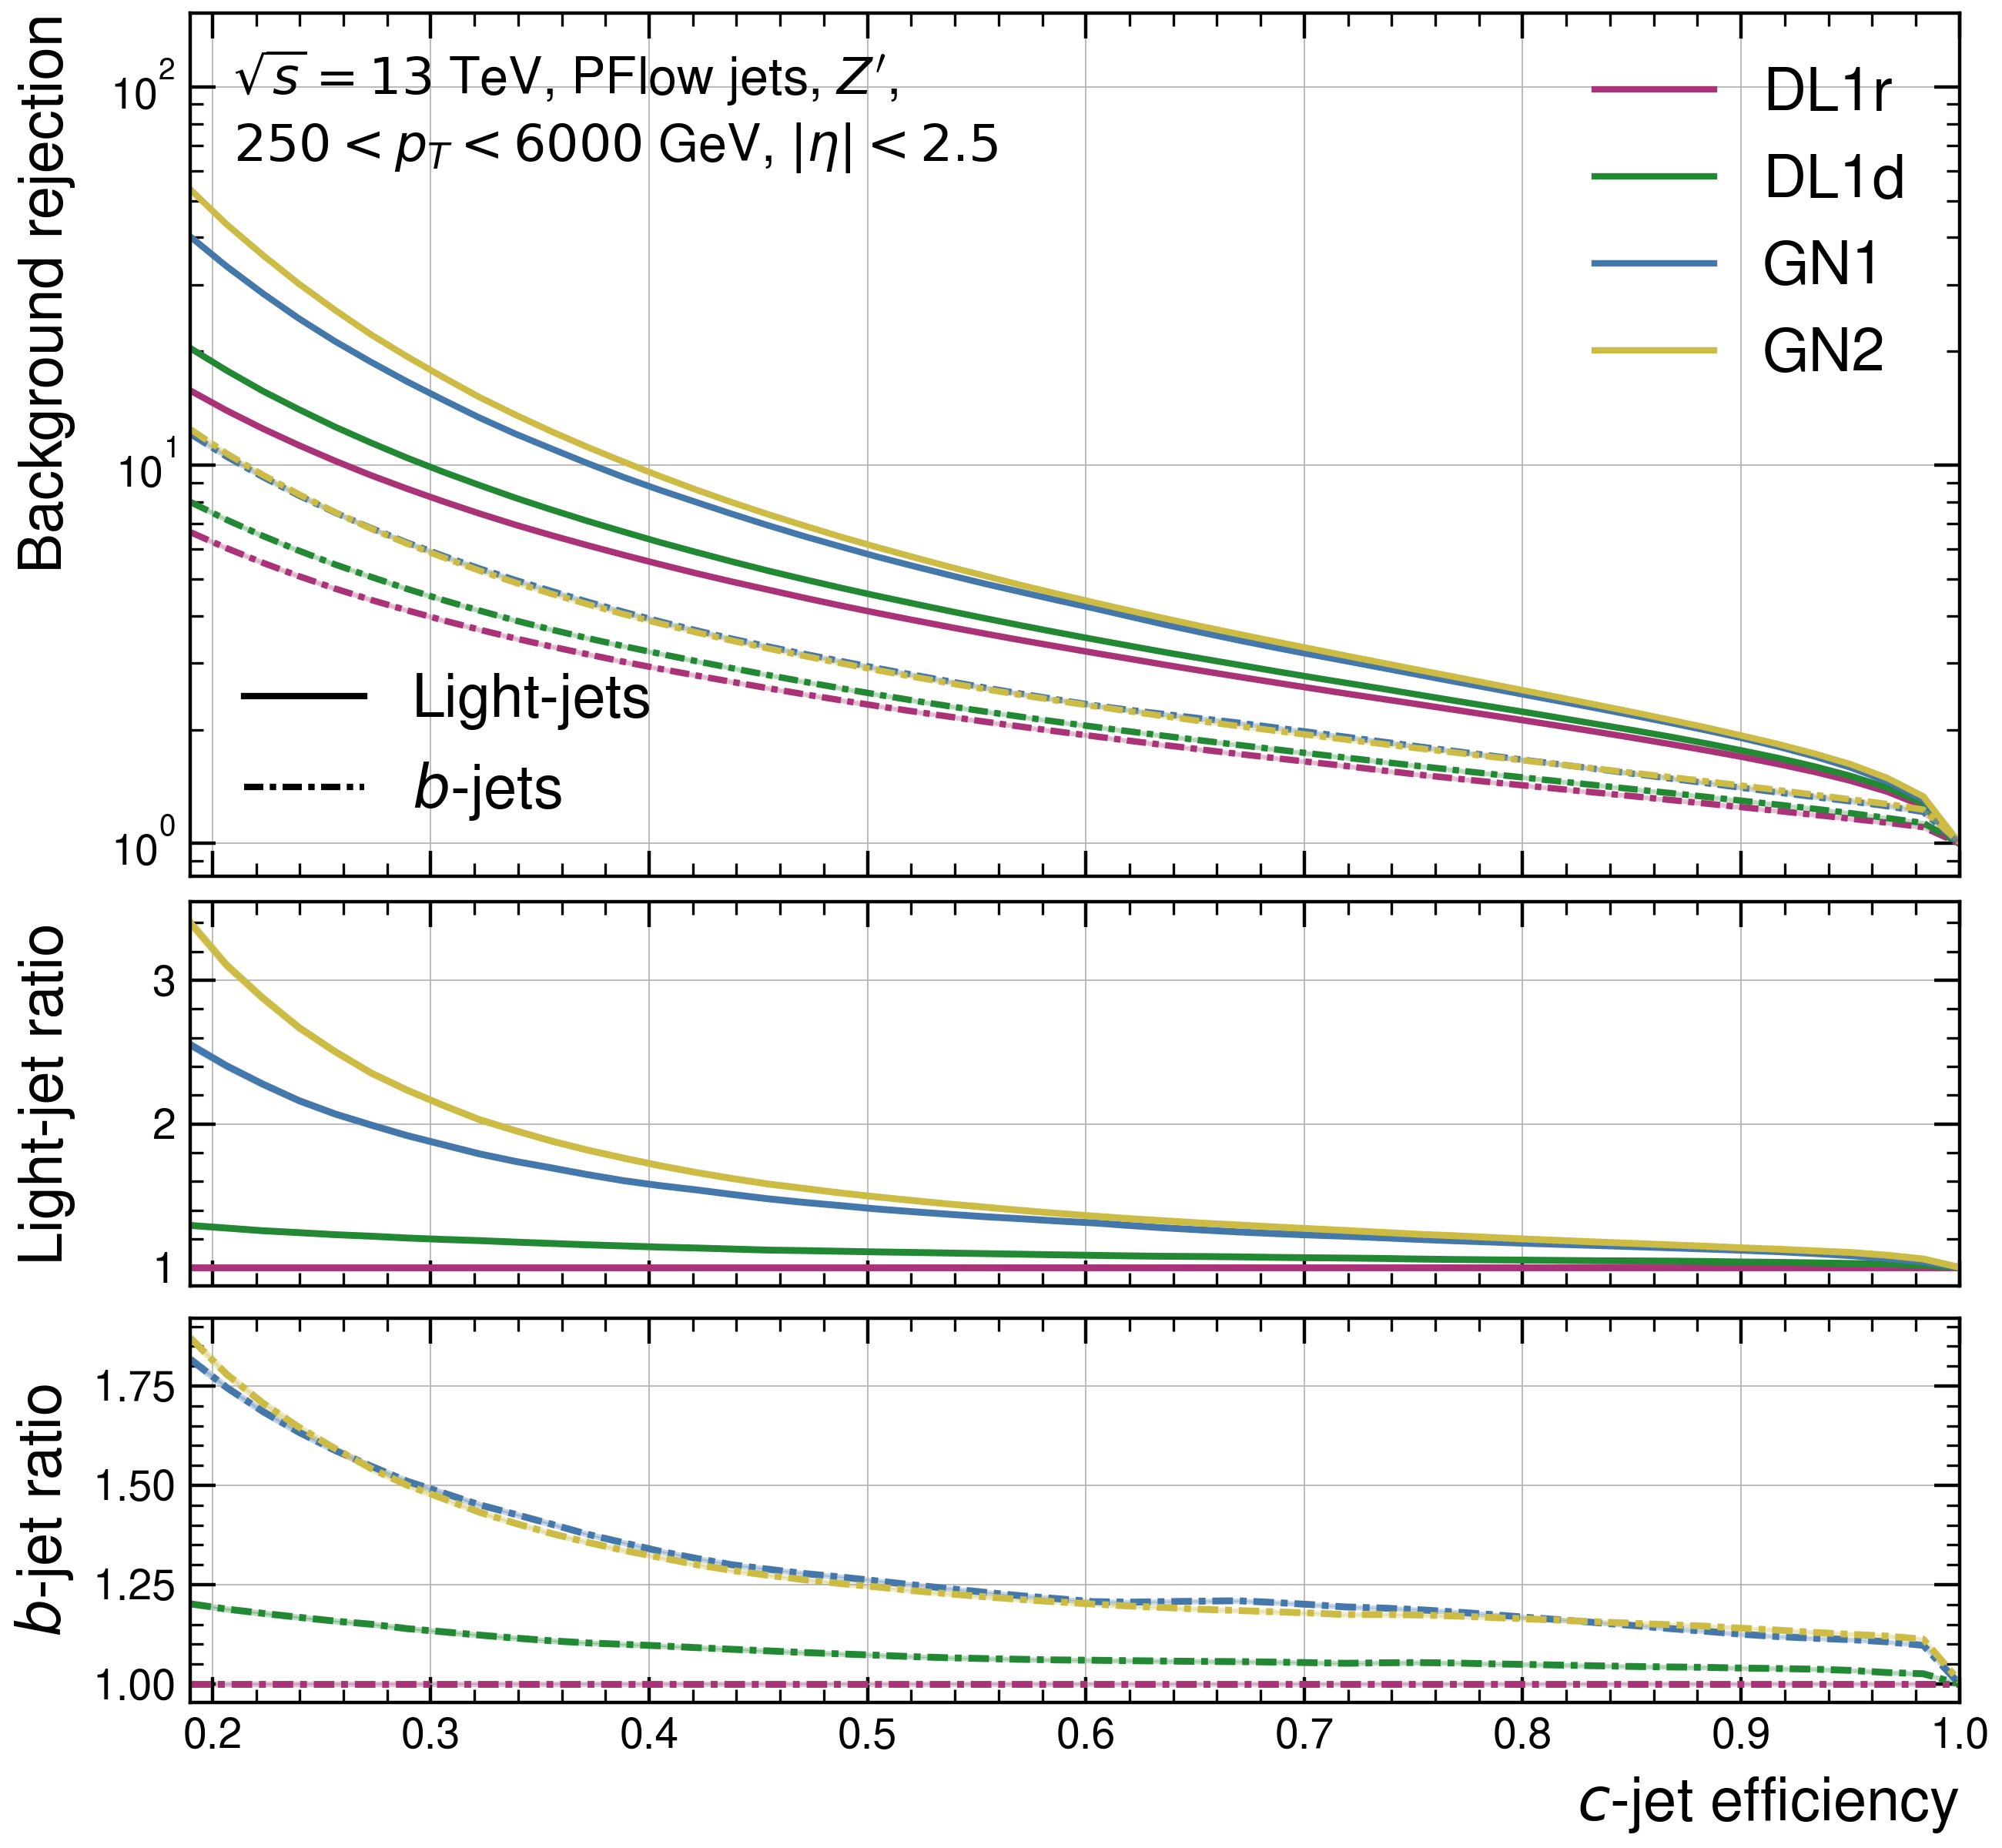
\includegraphics[width=0.50\textwidth]{Images/FTAG/GN/GN2/rocs/roc_zp_c.png}
  }
  \caption{The $b$- and light-rejections as a function of the $c$-jet tagging efficiency in the $t\bar{t}$ with $20 < p_T < 250$ GeV (left) and $Z'$ with $250 < p_T < 6000$ GeV (right) test samples. Models compared are DL1r in purple, DL1d in green, GN1 in blue, and GN2 in yellow. The bottom plots show the ratio with respect to the DL1d performance. Flavour fractions are set at $f^c_b = 0.2$ for all models. Shaded regions represent the binominal error band.}
  \label{fig:GN2rocc}
  \end{figure}
\end{center}

Fixing the $b$-tagging performance at the 77\% working point for both the $t\bar{t}$ and $Z'$, Figure \ref{fig:GNxscansfc} scans the $f^b_c$ flavour fractions for the different models. A clear hierarchy of performance is displayed by these four graphics: \gls{gn2} is occupies in an undisputed way the high rejections parts, followed by \gls{gn1}, \gls{dl1d}, and finally \gls{dl1r}. For $b$-tagging on $Z'$, the $c$-rejection could be further improved with limited impact on light-rejection by a larger $f^b_c$ choice. However, the flavour fractions are optimised for an improved $c$-rejection on $t\bar{t}$, with limited change to the light-rejection across tagger generations. If desired, the light-rejection on $t\bar{t}$ of a \gls{gn2} taggers could be push upwards by lowering the $f^b_c$, reaching values as high as 1800 at a $c$-rej of 4.8. The equivalent \gls{dl1d} performance is a light-rejection of 450 at a $c$-rejection of 4.5, equivalent 25\% of the \gls{gn2} light-rejection. Similarly, \gls{gn2} can reach a $c$-rejection of 19.5 at a ligh-rejection of 110, compared to a maximal $c$-rejection of 9.7 for a light-rejection of 40. \\

\begin{figure}[h!]
  \centering
  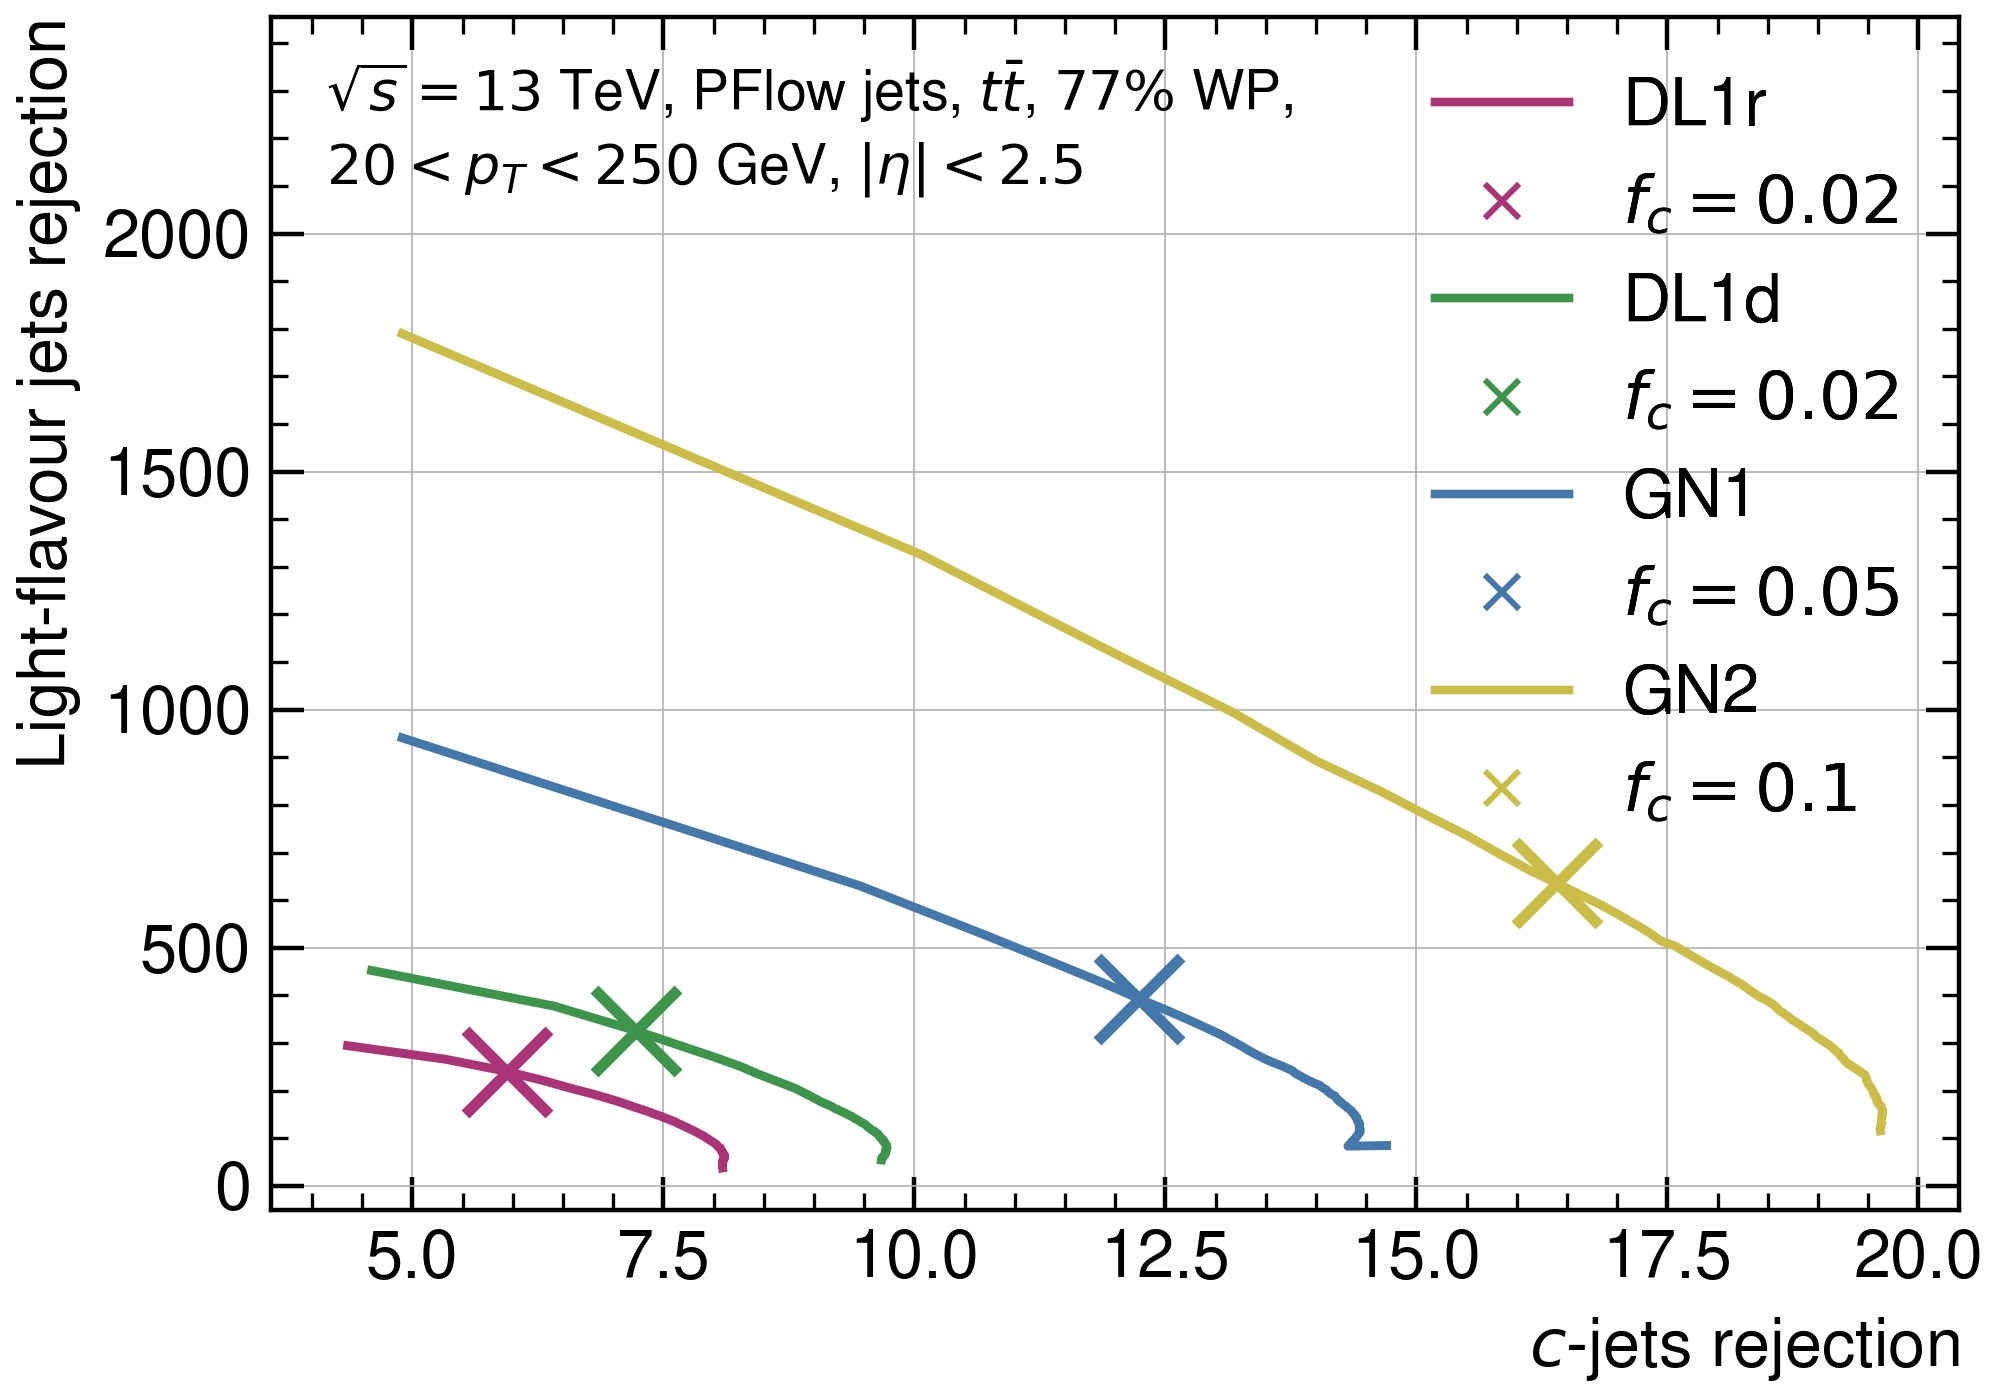
\includegraphics[width=0.48\textwidth]{Images/FTAG/GN/GN2/fraction_scans/FractionScanPlot_tt.png}
  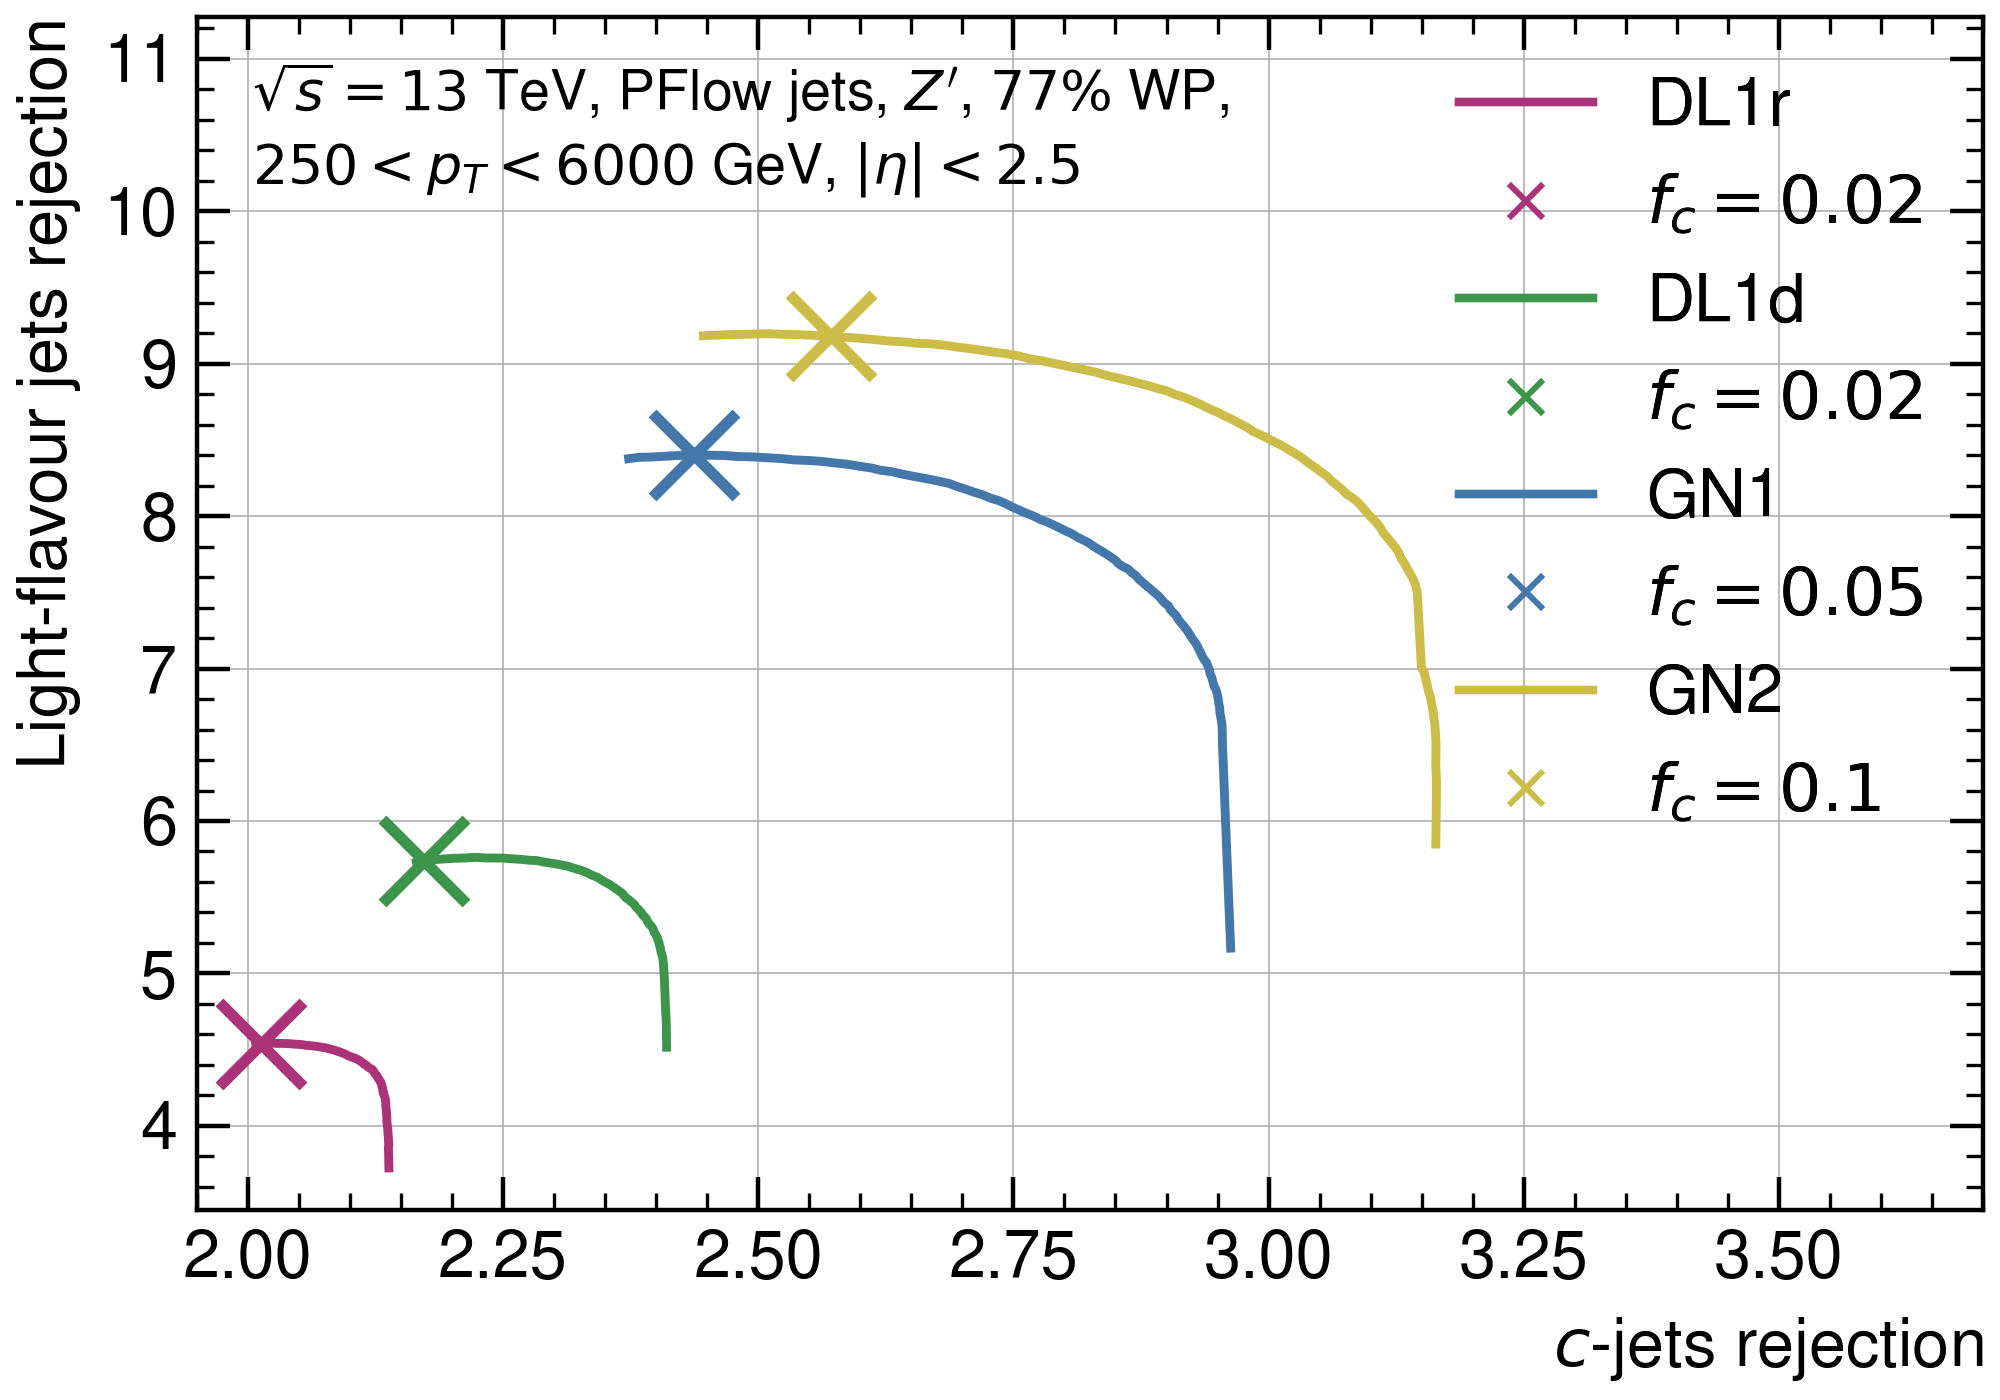
\includegraphics[width=0.48\textwidth]{Images/FTAG/GN/GN2/fraction_scans/FractionScanPlot_zp.png}
  \caption{The flavour fraction $f^b_c$ scans for $b$-tagging at a fixed working point of 77\% of the different models considered evaluated on the $t\bar{t}$ (left) and $Z'$ (right). The chosen values are marked on the curves, displaying on the $x$-axis the $c$-rejection vs the light-rejection on the $y$ axis. Increasing $f^b_c$ shifts the marker rightwards along the curves. }
  \label{fig:GNxscansfc}
\end{figure} 

Figure \ref{fig:GNxscansfb} displays the flavour fraction $f^c_b$ scans for $c$-tagging at the 30\% working point. The same conclusions as for $b$-tagging holds, underlying the overall superiority of \gls{gn2}. The scans for $c$-tagging show a different pattern than the $b$-tagging ones: at large $f^c_b$, the $b$-rejection rapidly increases while for $b$-tagging the $c$-rejection was saturating. This behaviour is due to the clear identification of $b$-jets giving them an outlying distribution compared to the overlap of $c$- and light-jets. \\

\begin{figure}[h!]
  \centering
  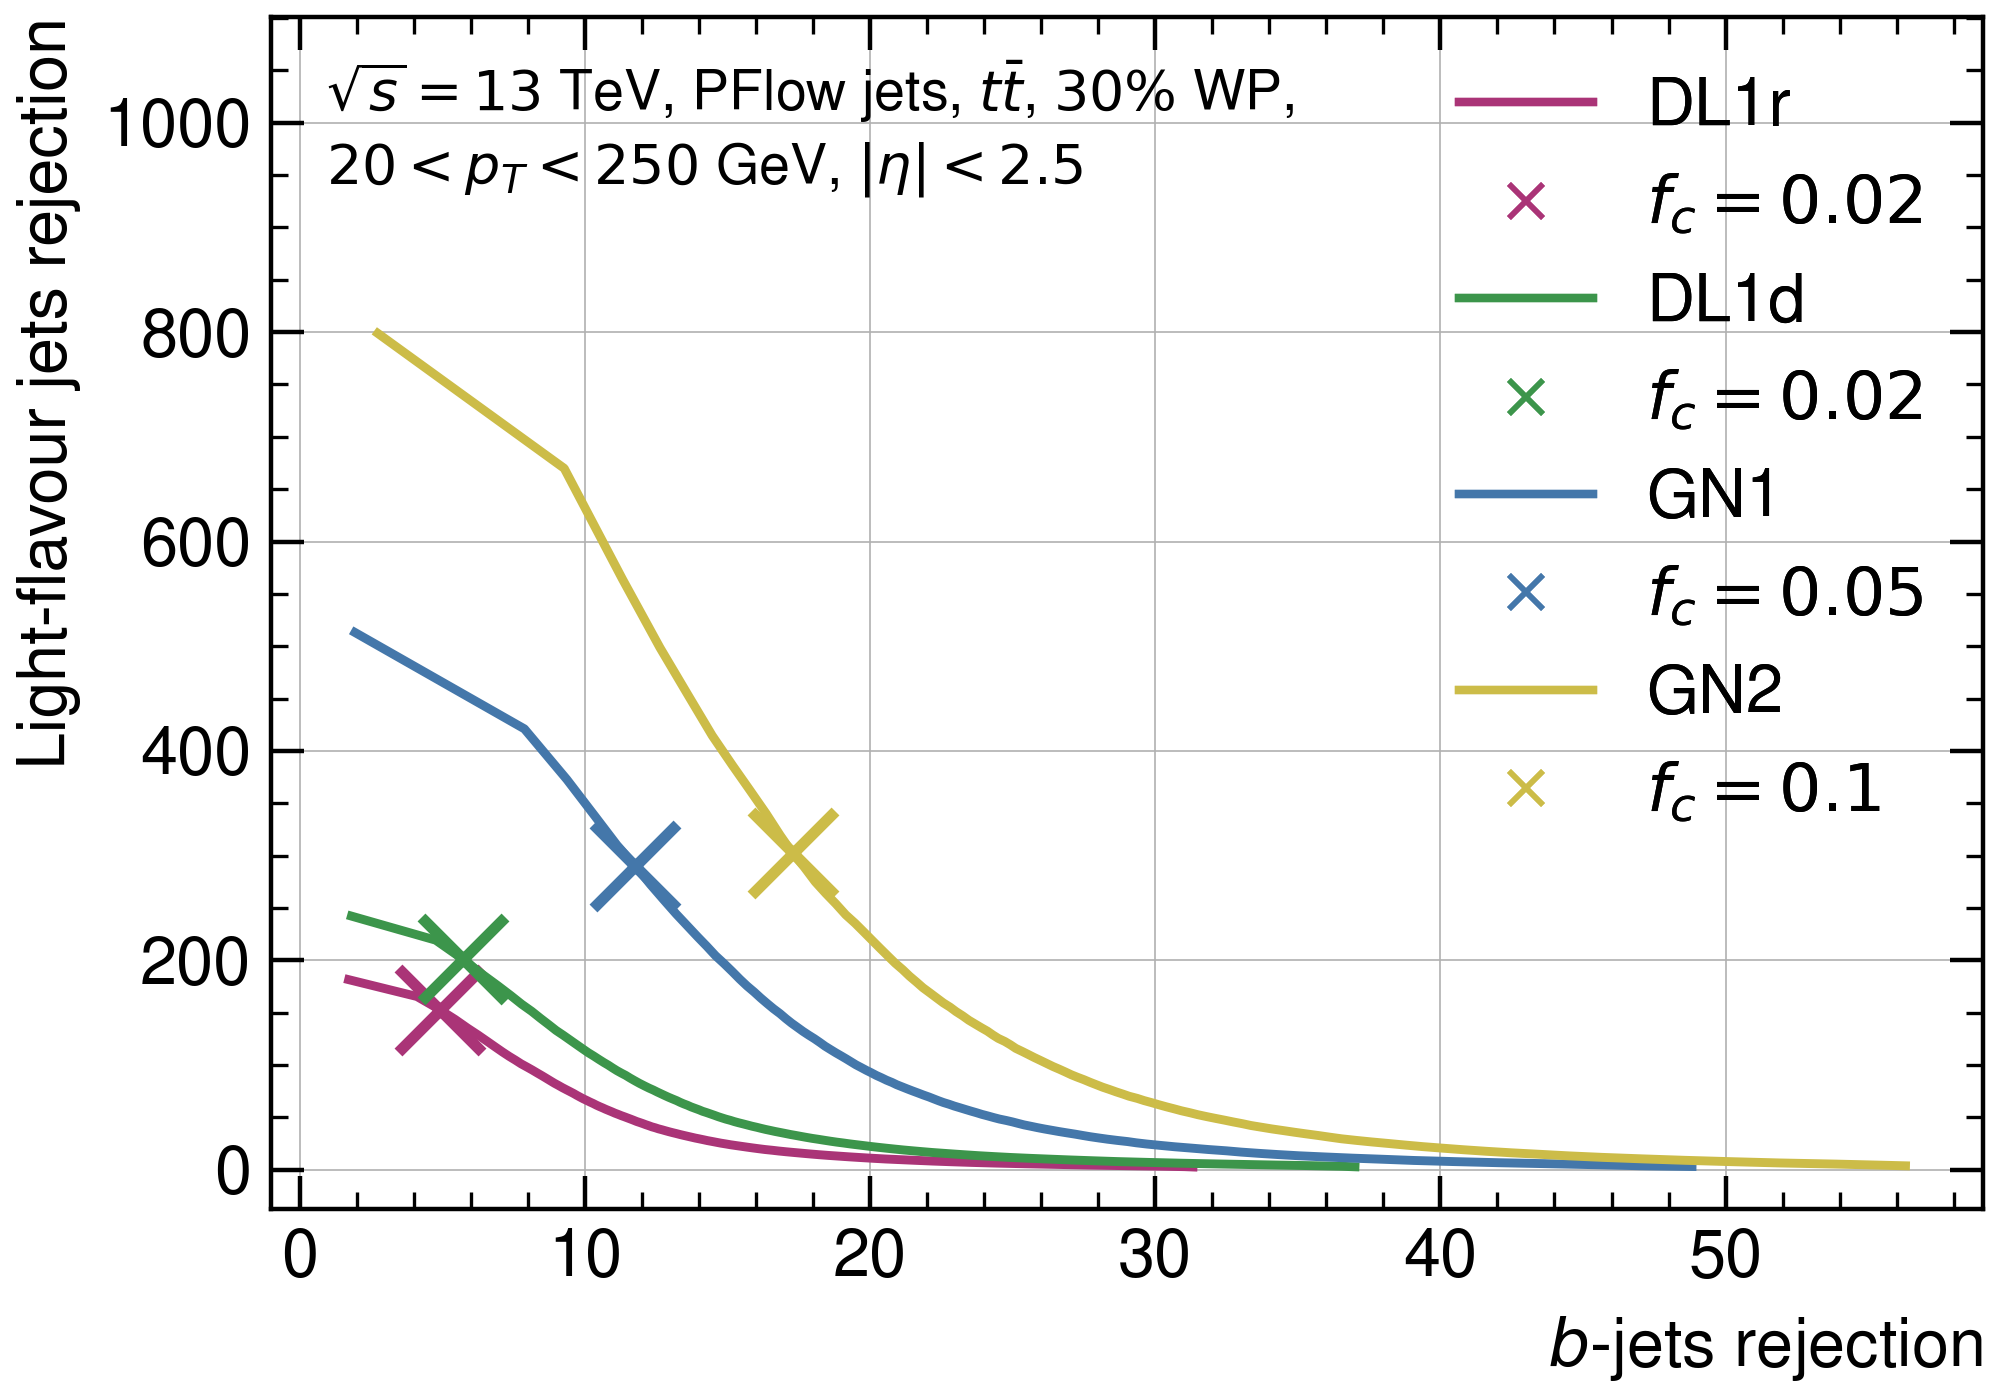
\includegraphics[width=0.48\textwidth]{Images/FTAG/GN/GN2/fraction_scans/FractionScanPlot_tt_c.png}
  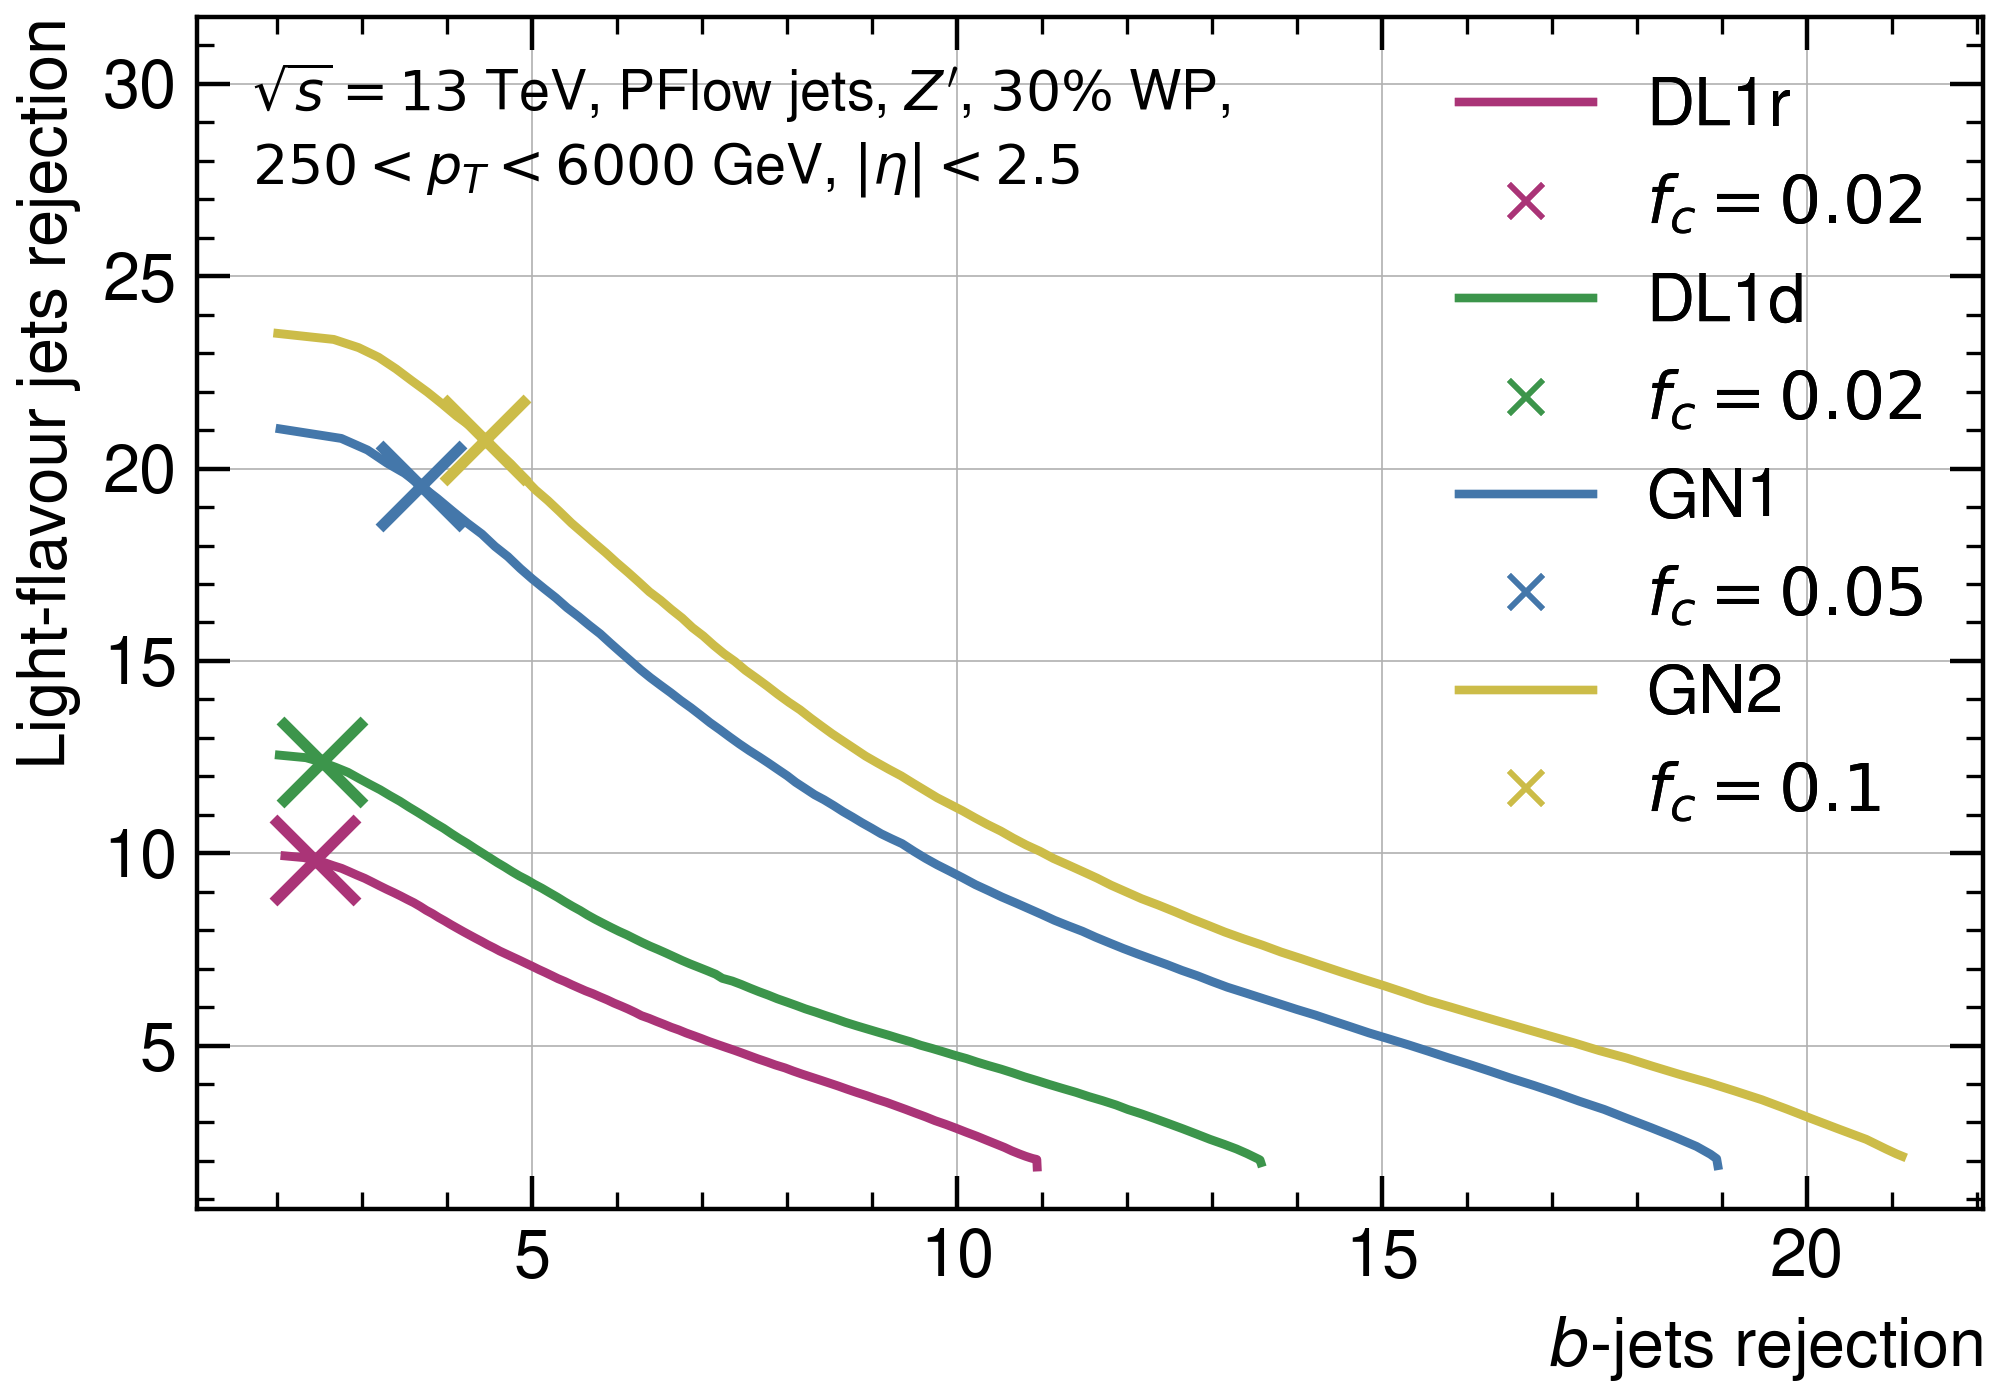
\includegraphics[width=0.48\textwidth]{Images/FTAG/GN/GN2/fraction_scans/FractionScanPlot_zp_c.png}
  \caption{The flavour fraction $f^c_b$ scans for $c$-tagging at a fixed working point of 30\% of the different models considered evaluated on the $t\bar{t}$ (left) and $Z'$ (right). The chosen values are marked on the curves, displaying on the $x$-axis the $b$-rejection vs the light-rejection on the $y$ axis. Increasing $f^c_b$ shifts the marker rightwards along the curves. }
  \label{fig:GNxscansfb}
\end{figure} 

% Eff for fixed WP
Figure \ref{fig:GNxptb_eff} displays the effective per bin $b$-tagging efficiency for inclusive $b$-tagging efficiency of 70\% for $t\bar{t}$ and 30\% for $Z'$ in each $p_T$ region considered. The performance is visibly not uniform across $p_T$, with teh model accomodating specific parts of the $p_T$ spectrum more easily. The region [100, 800] GeV overlapping the two samples is a sweet spot for performance, with more challenging results at lower and higher $p_T$. The performance for $Z'$ in particular reduces dramatically with larger momentum, due to the physics reasons previously explained. Figure \ref{apfig:GNxptc_eff} in Appendix \ref{app-GN2sup} displays the same information for $c$-tagging, leading to the same conclusions. 
\begin{figure}[h!]
  \centering
  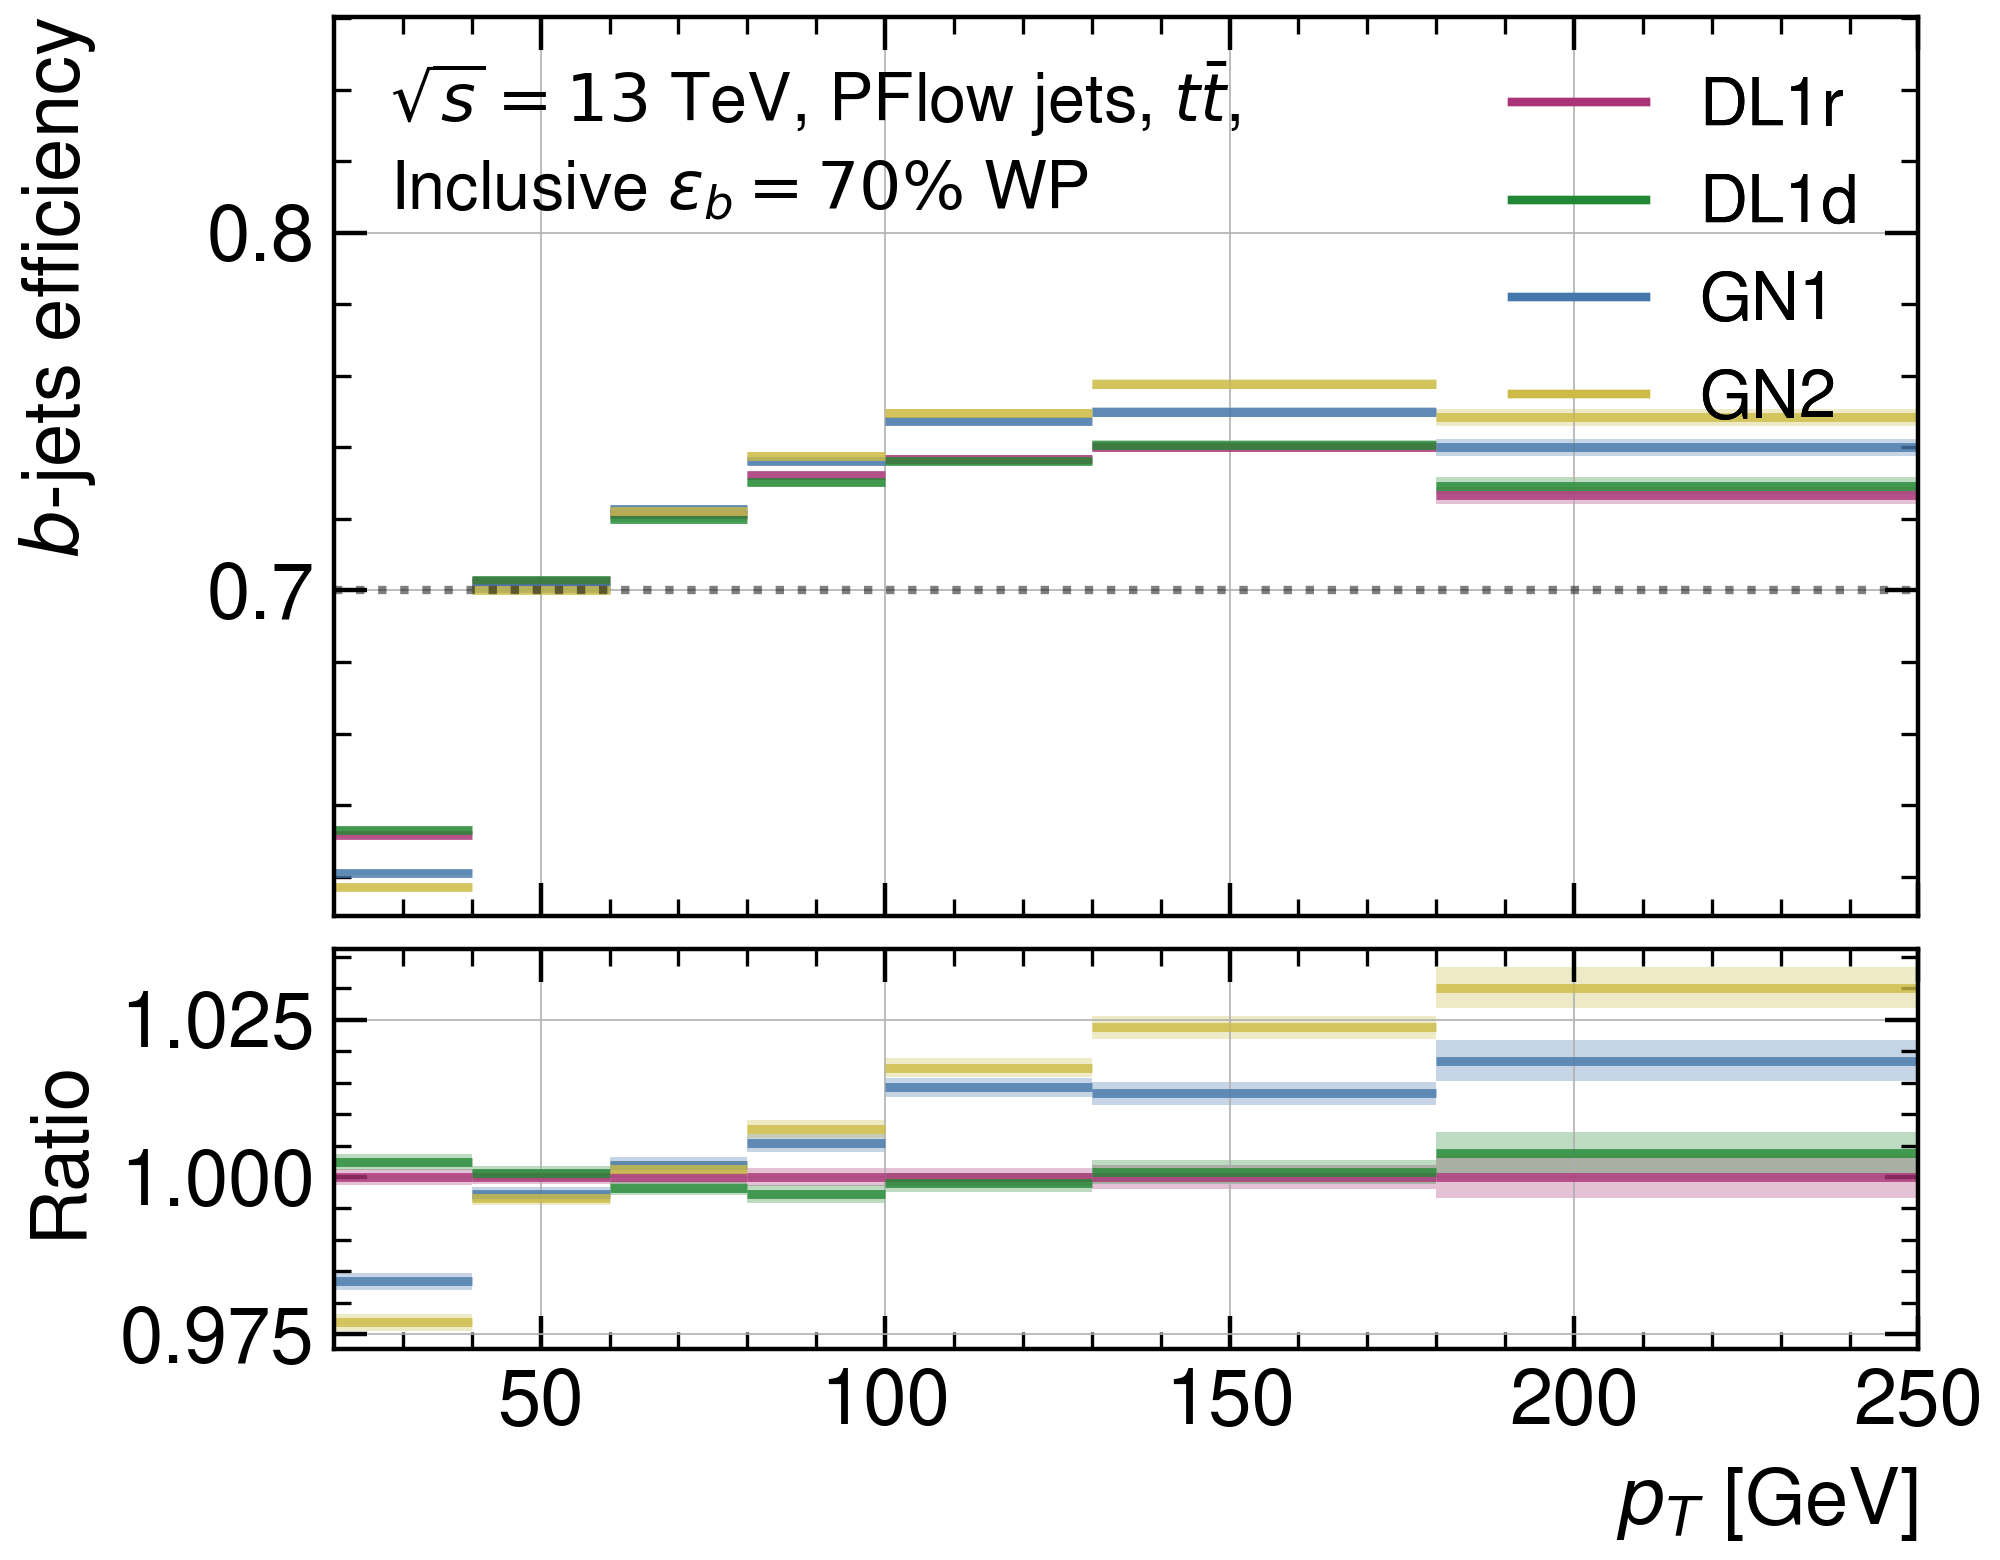
\includegraphics[width=0.48\textwidth]{Images/FTAG/GN/GN2/pt_plots/pt_ttbar_b_eff.png}
  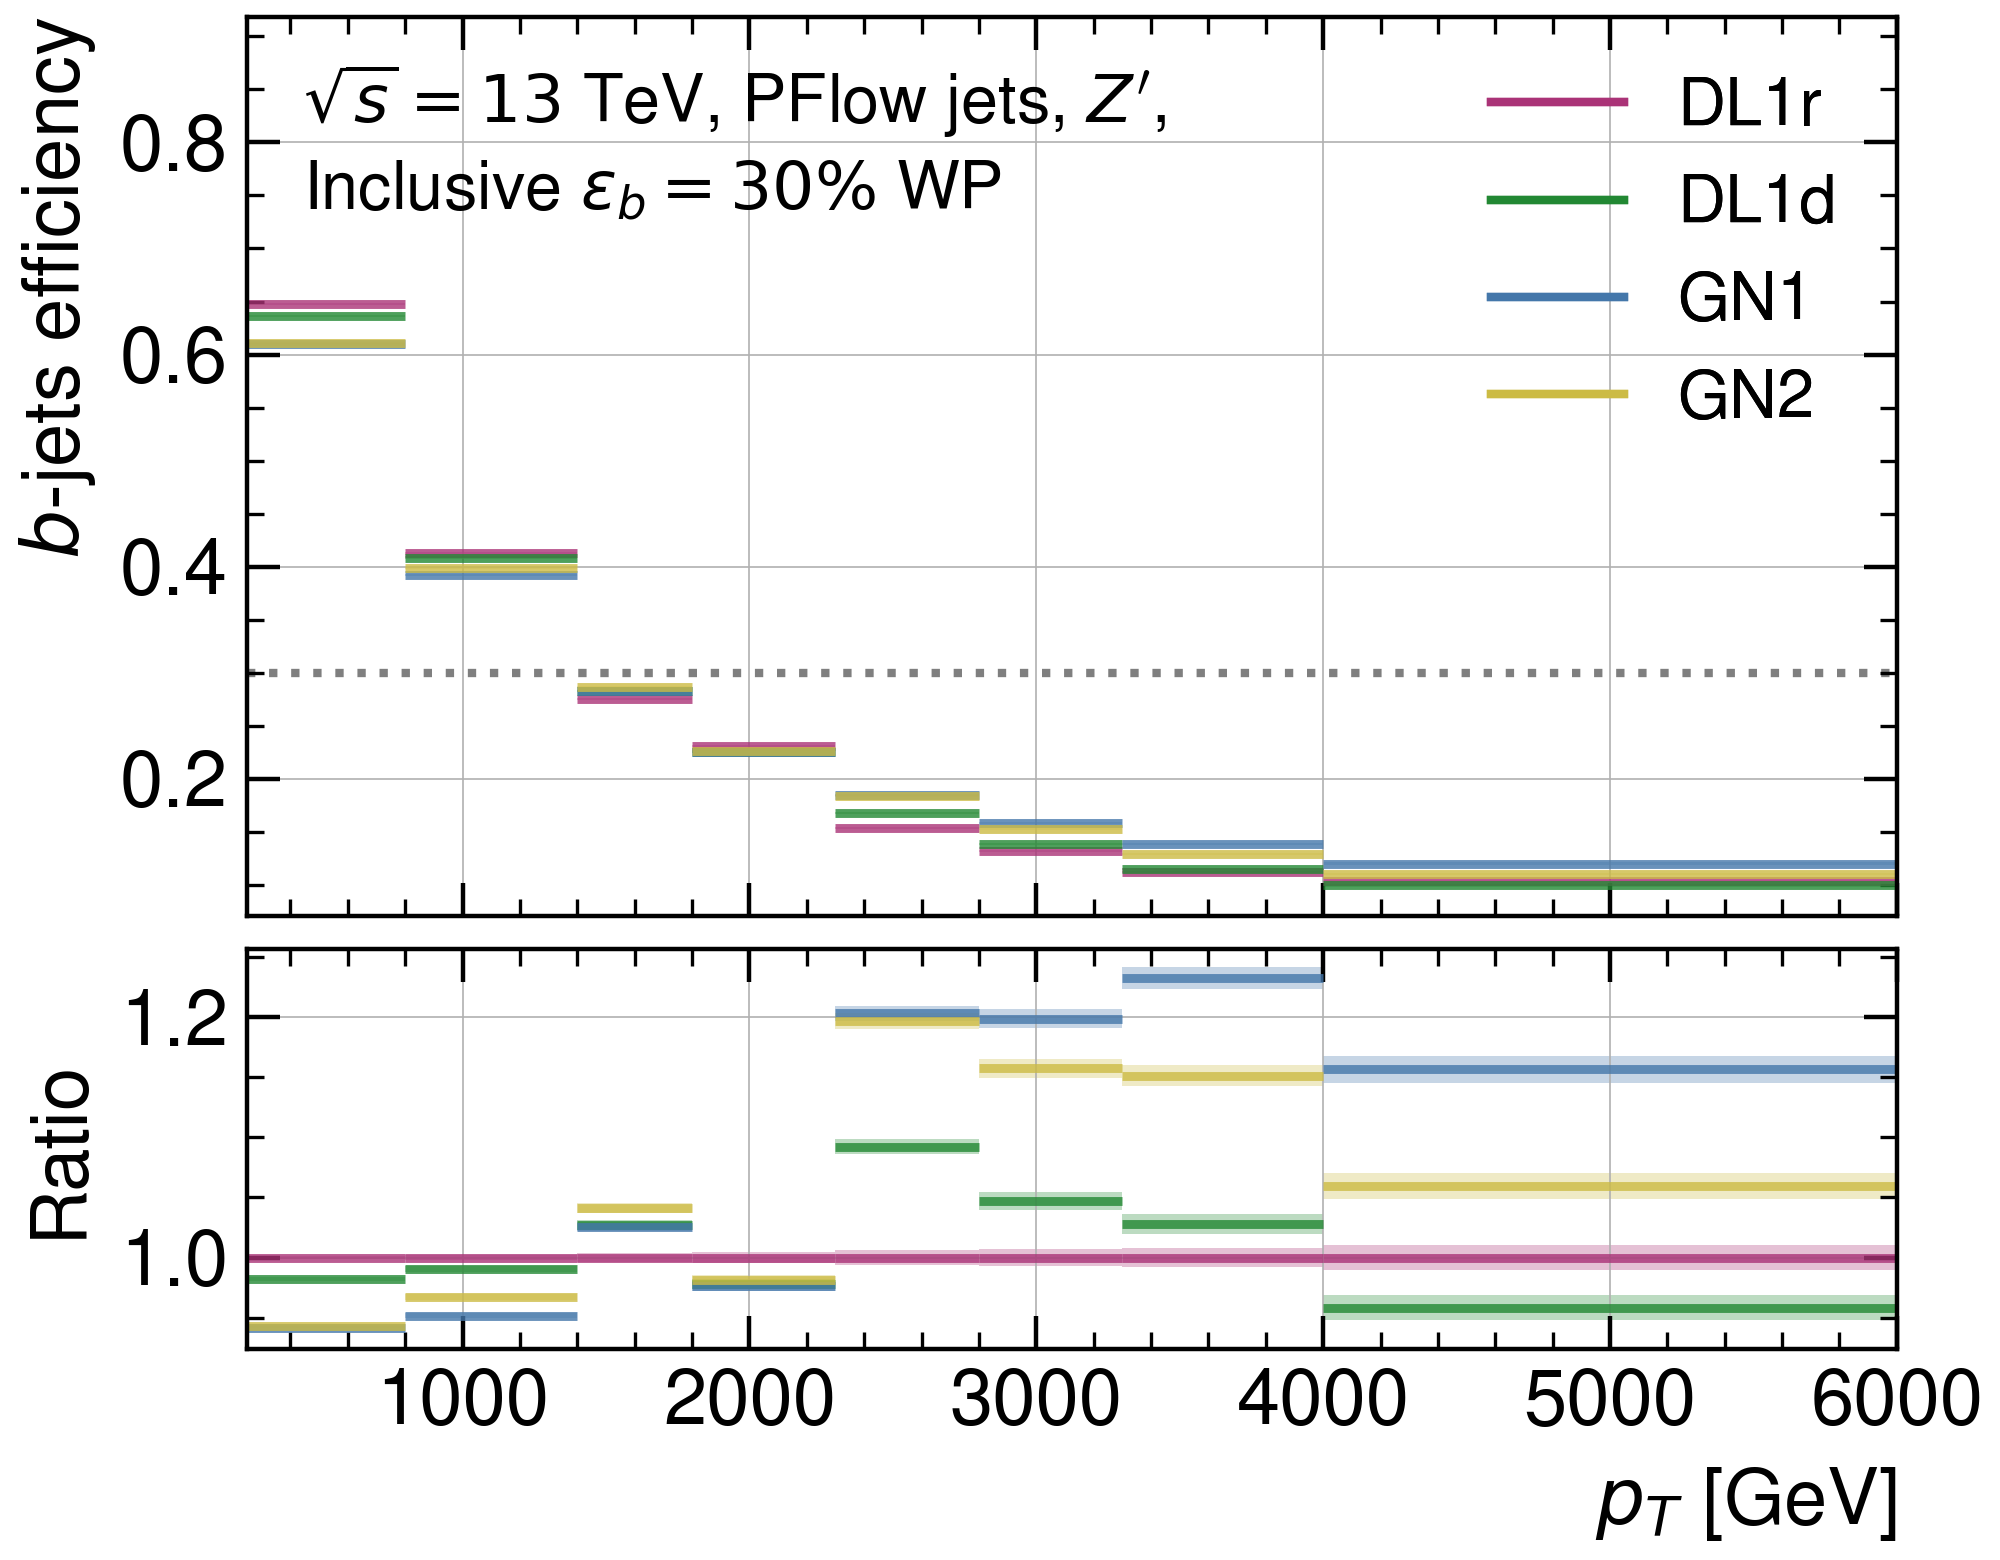
\includegraphics[width=0.48\textwidth]{Images/FTAG/GN/GN2/pt_plots/pt_zp_b_eff.png}
  \caption{Comparing the different models $b$-tagging efficiency as a function of jet $p_T$ for the inclusive $b$-tagging 70\% working point on the $t\bar{t}$ (left) and 30\% working point on $Z'$ (right). The flavour fraction is set at $f^b_c = 0.018$ for DL1r and DL1d, 0.05 for GN1, and 0.1 for GN2.}
  \label{fig:GNxptb_eff}
\end{figure} 

To avoid biasing the analysis with this per-bin performance dependency, Figure \ref{fig:GNxptb_efffixedl} displays the $b$-tagging efficiency distribution across $p_T$ at a fixed per bin light-rejection of 100. The superior capabilities of \gls{gn2} are clearly exhibited across the $p_T$ spectrum. The same conclusion holds for $c$-tagging, as displayed in Figure \ref{apfig:GNxptc_efffixedl} of the appendix. 
% Eff fixed light
\begin{figure}[h!]
  \centering
  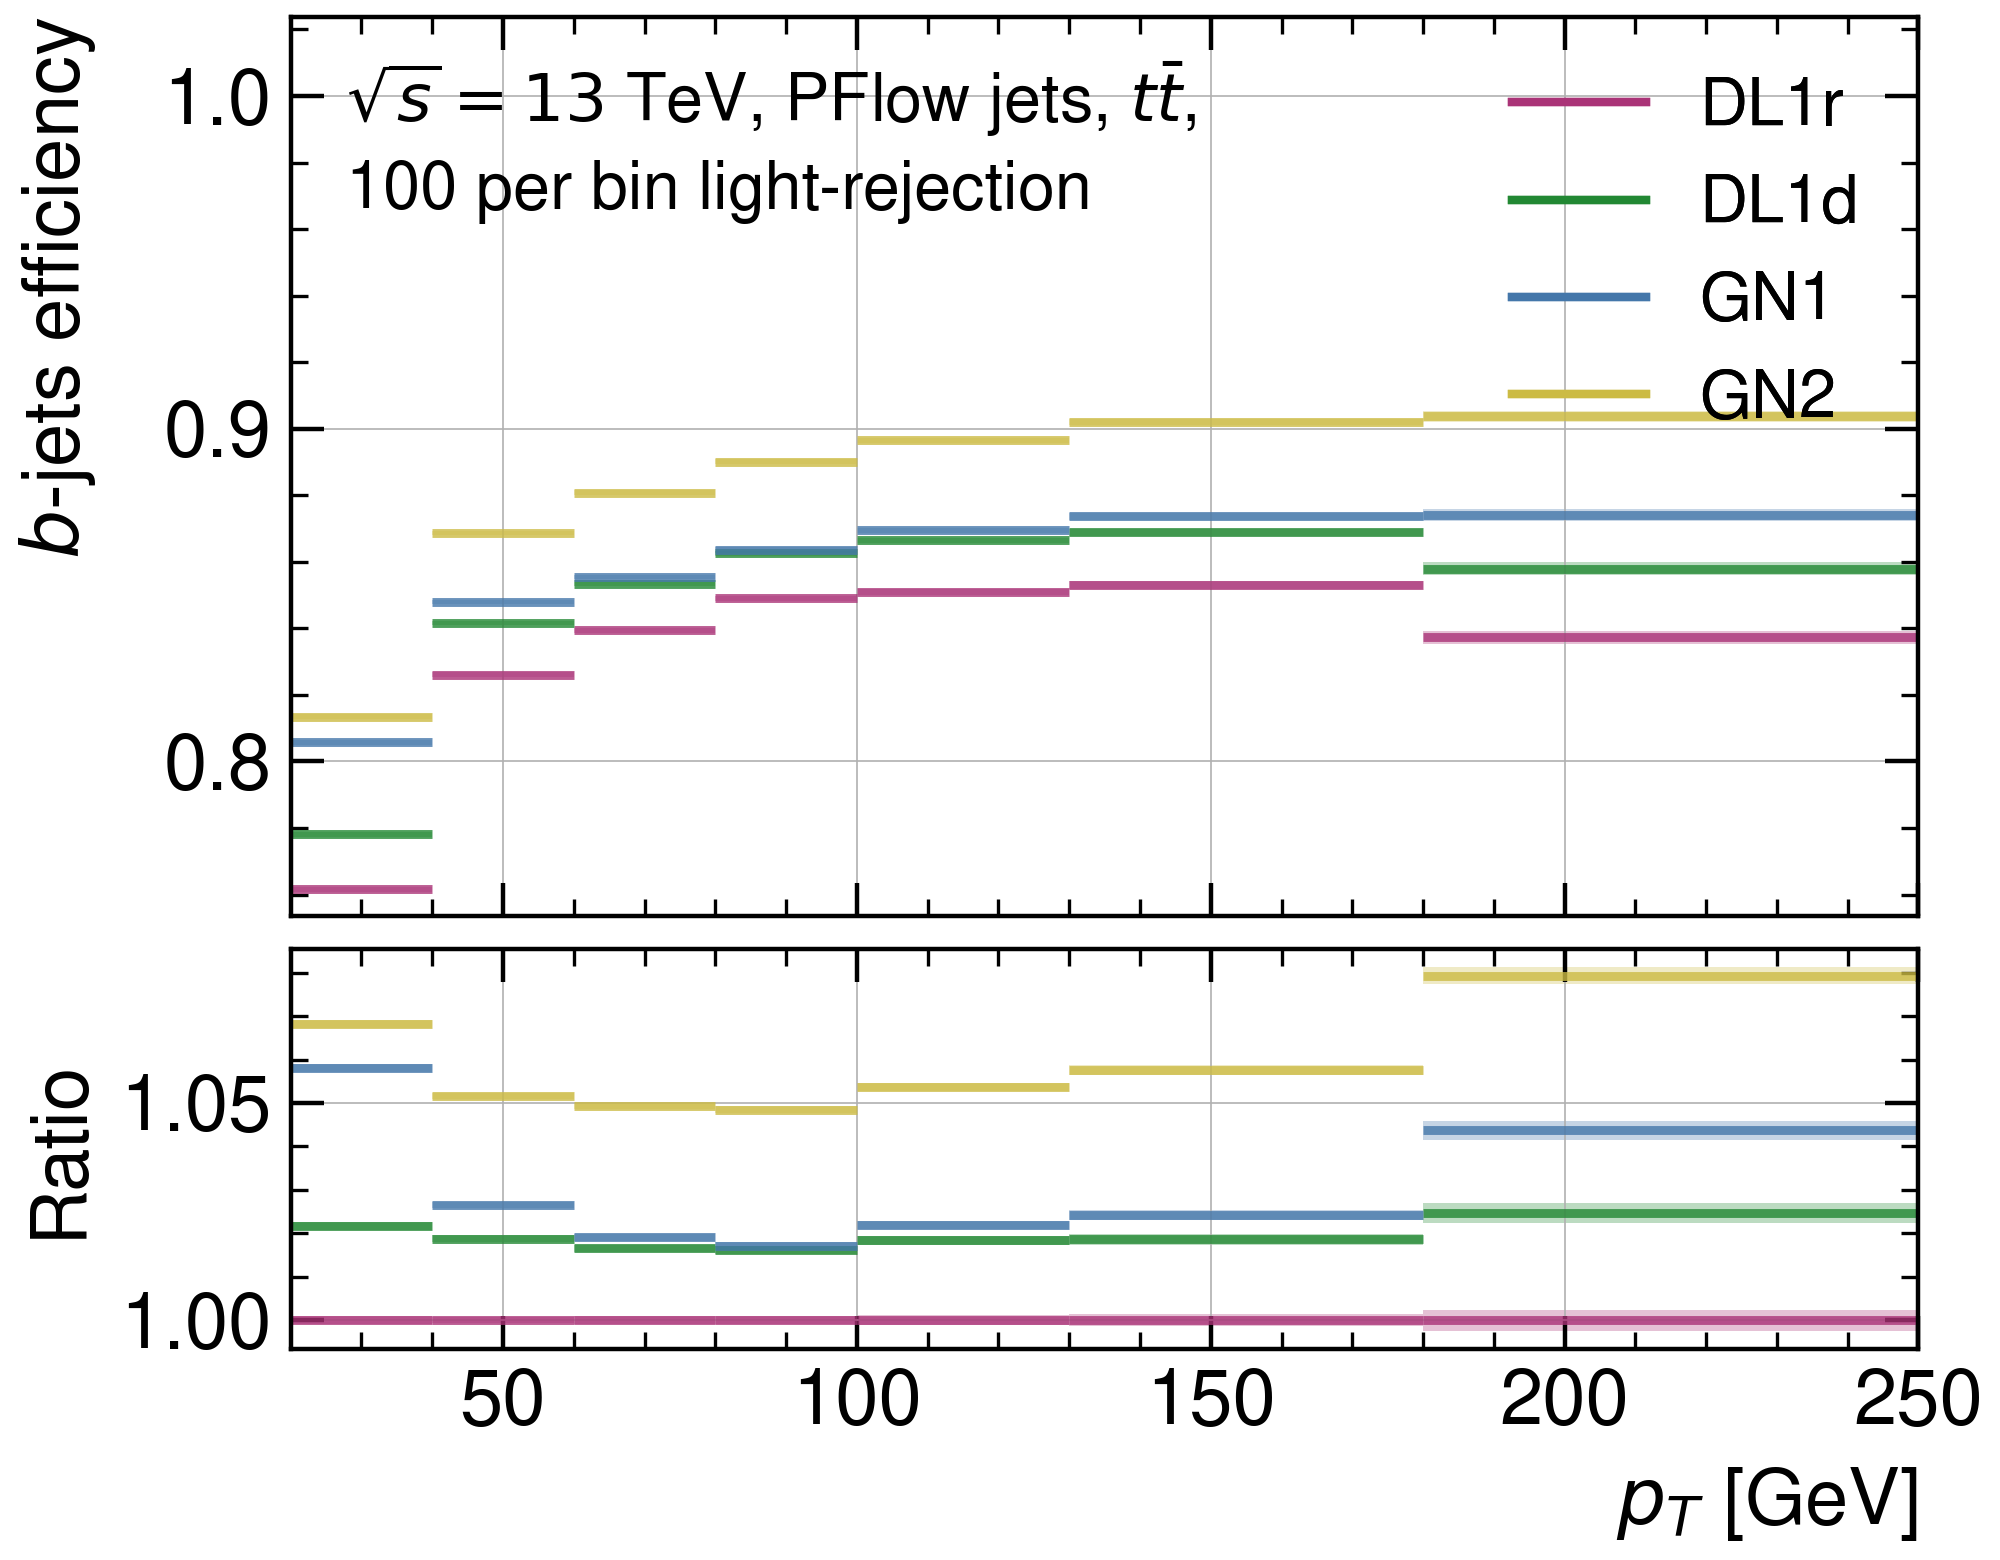
\includegraphics[width=0.48\textwidth]{Images/FTAG/GN/GN2/pt_plots/pt_ttbar_b_eff_fixedlight.png}
  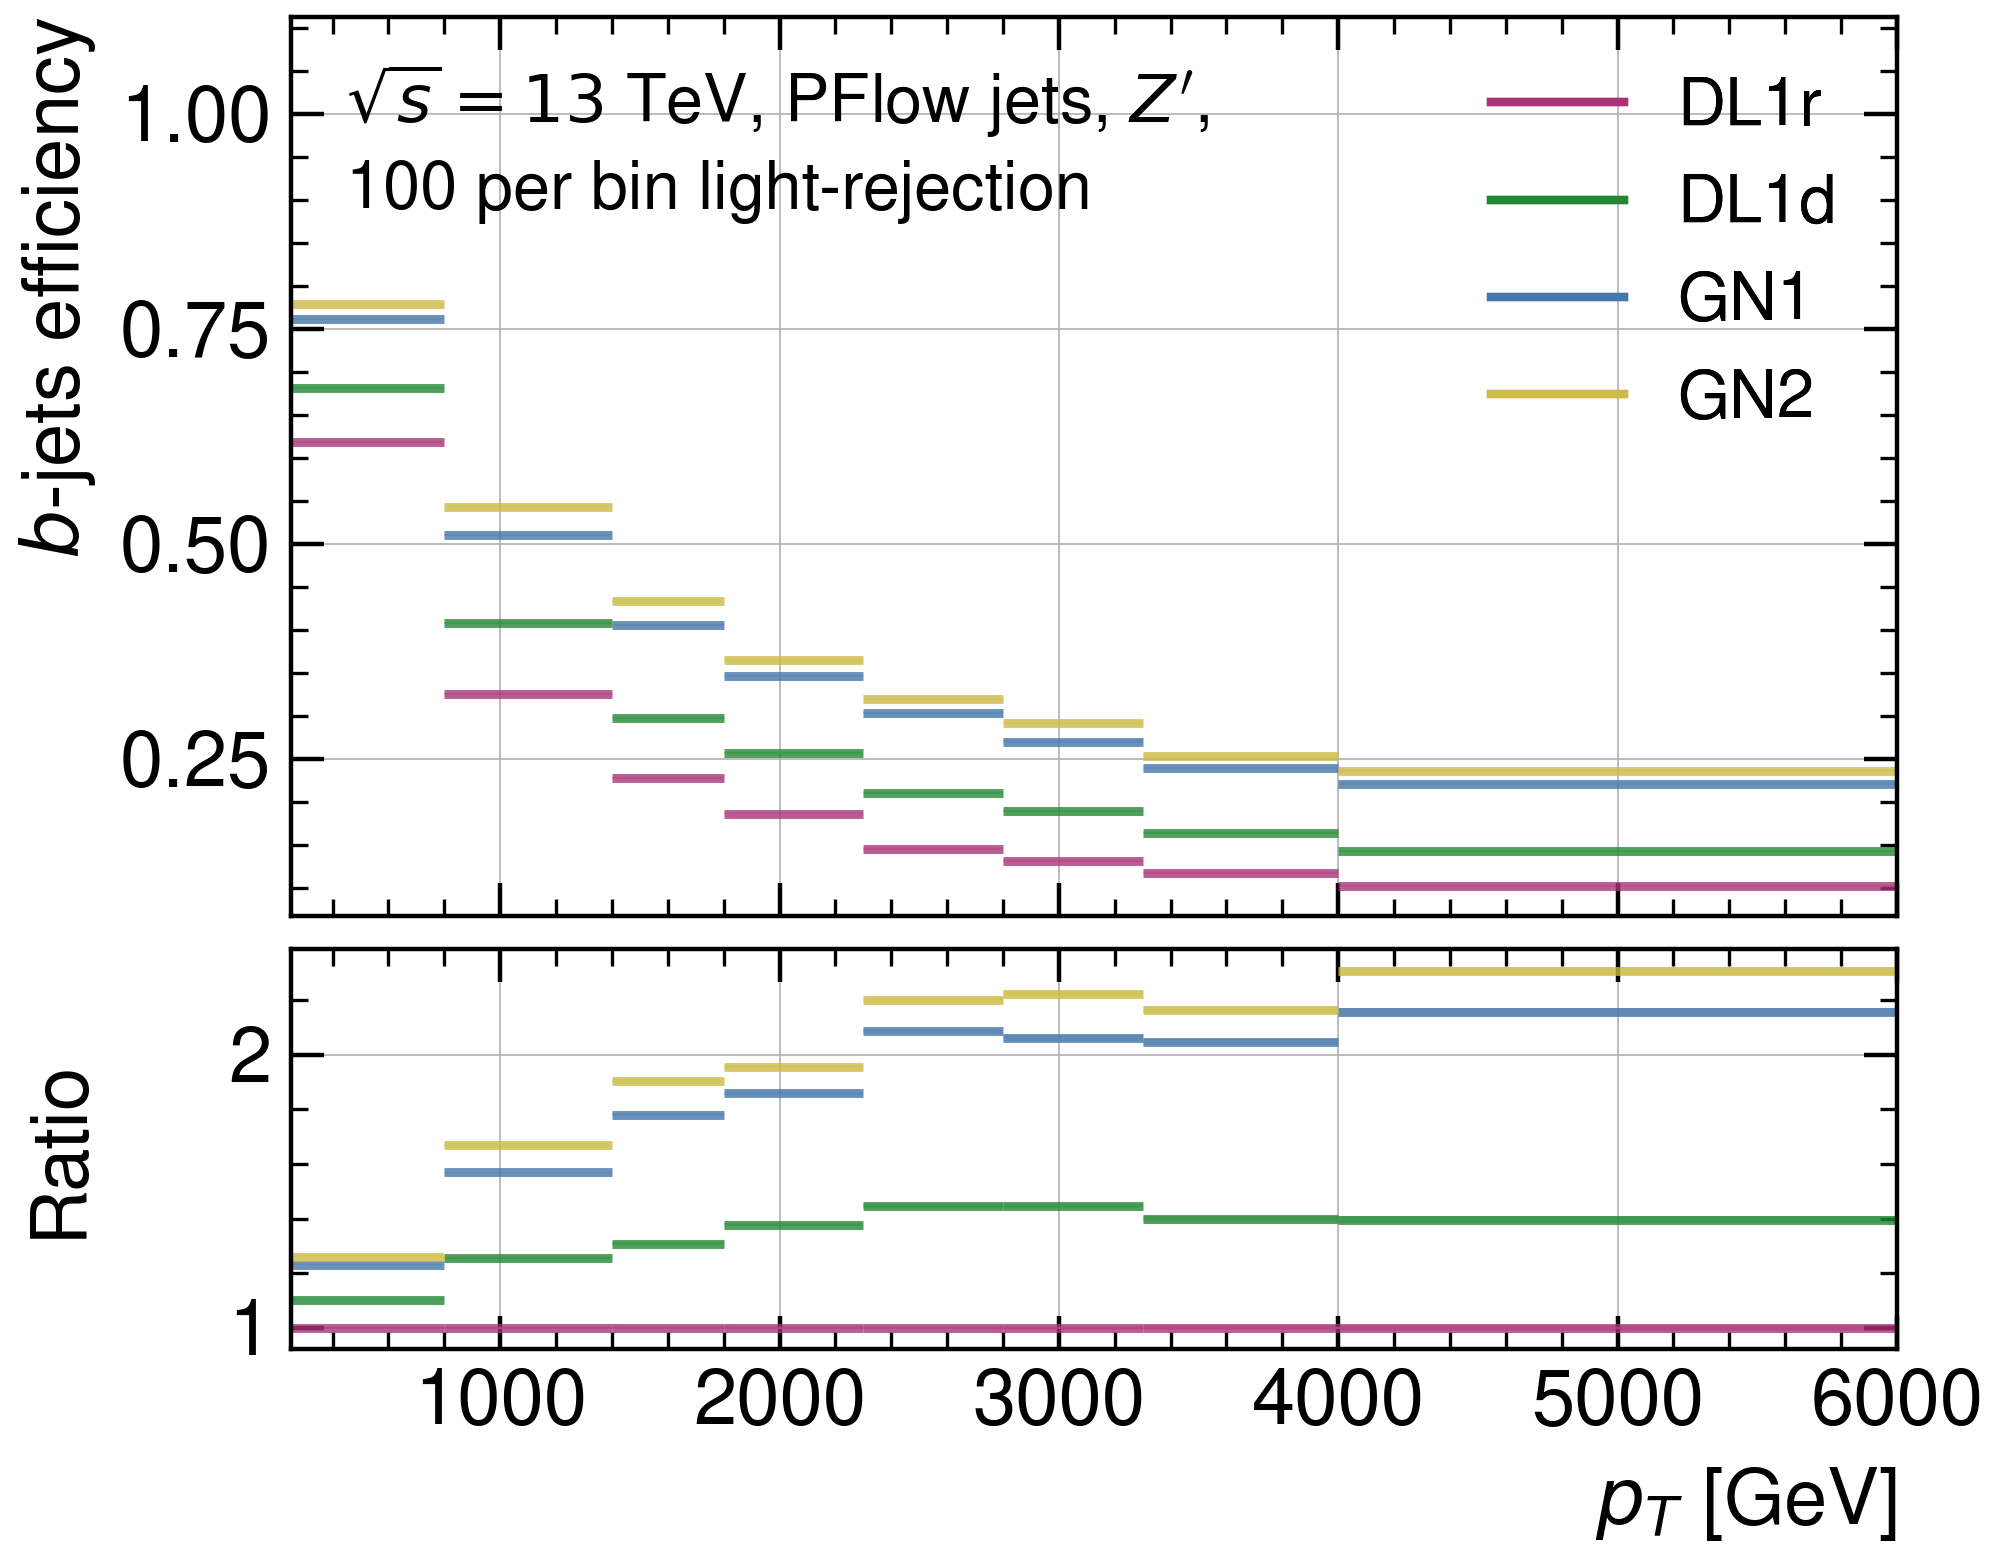
\includegraphics[width=0.48\textwidth]{Images/FTAG/GN/GN2/pt_plots/pt_zp_b_eff_fixedlight.png}
  \caption{Comparing the different models $b$-tagging efficiency as a function of jet $p_T$ at a fixed 100 light-jet rejection per bin on the $t\bar{t}$ (left) and $Z'$ (right) test samples. The flavour fraction is set at $f^b_c = 0.018$ for DL1r and DL1d, 0.05 for GN1, and 0.1 for GN2.}
  \label{fig:GNxptb_efffixedl}
\end{figure} 

Inspecting the rejections at a fixed $b$-tagging efficiency of 70\% per bin also leads to concluding the clear superiority of \gls{gn2}. Figures \ref{fig:GNxptb_crejflat} and \ref{fig:GNxptb_urejflat} respectively display the $c$- and light-rejection for a 70\% $b$-efficiency per bin, showing that most of the improvement from \gls{gn2} and \gls{gn1} is in the [100, 800] GeV $p_T$ sweetspot. The same distribution with an inclusive 70\% $b$-tagging efficiency, over the entire $p_T$ regions, are displayed in Figures \ref{apfig:GNxptb_crej} and \ref{apfig:GNxptb_urej} of the appendix. 

% Rej c - flat btagging
\begin{figure}[h!]
  \centering
  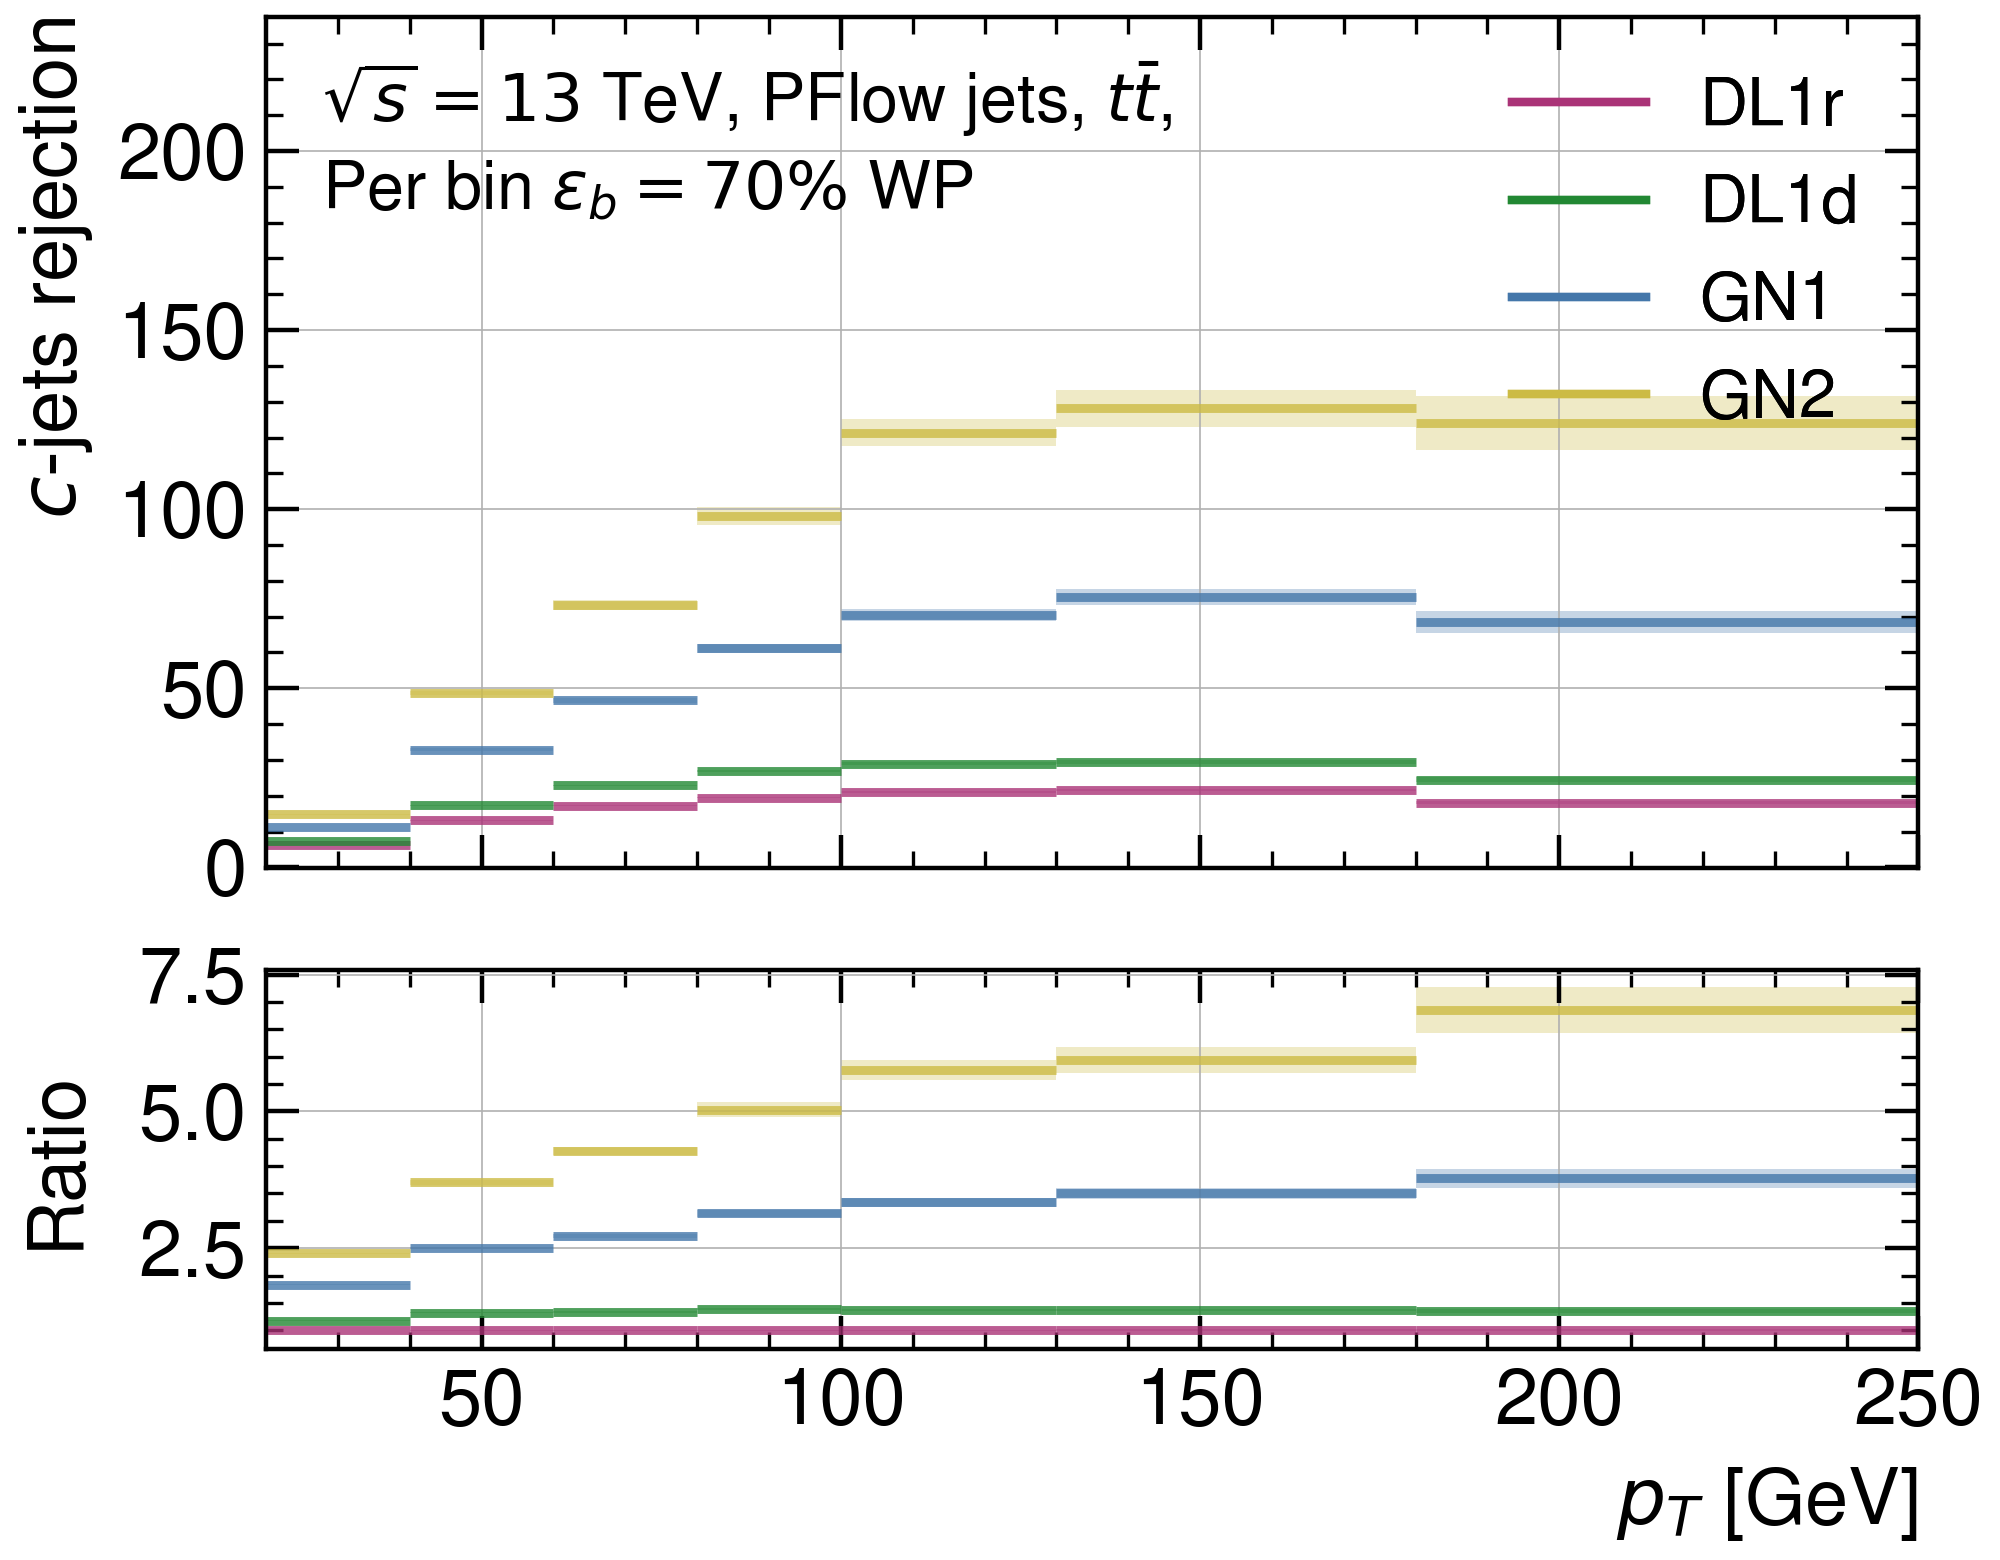
\includegraphics[width=0.48\textwidth]{Images/FTAG/GN/GN2/pt_plots/pt_ttbar_flat_c_rej.png}
  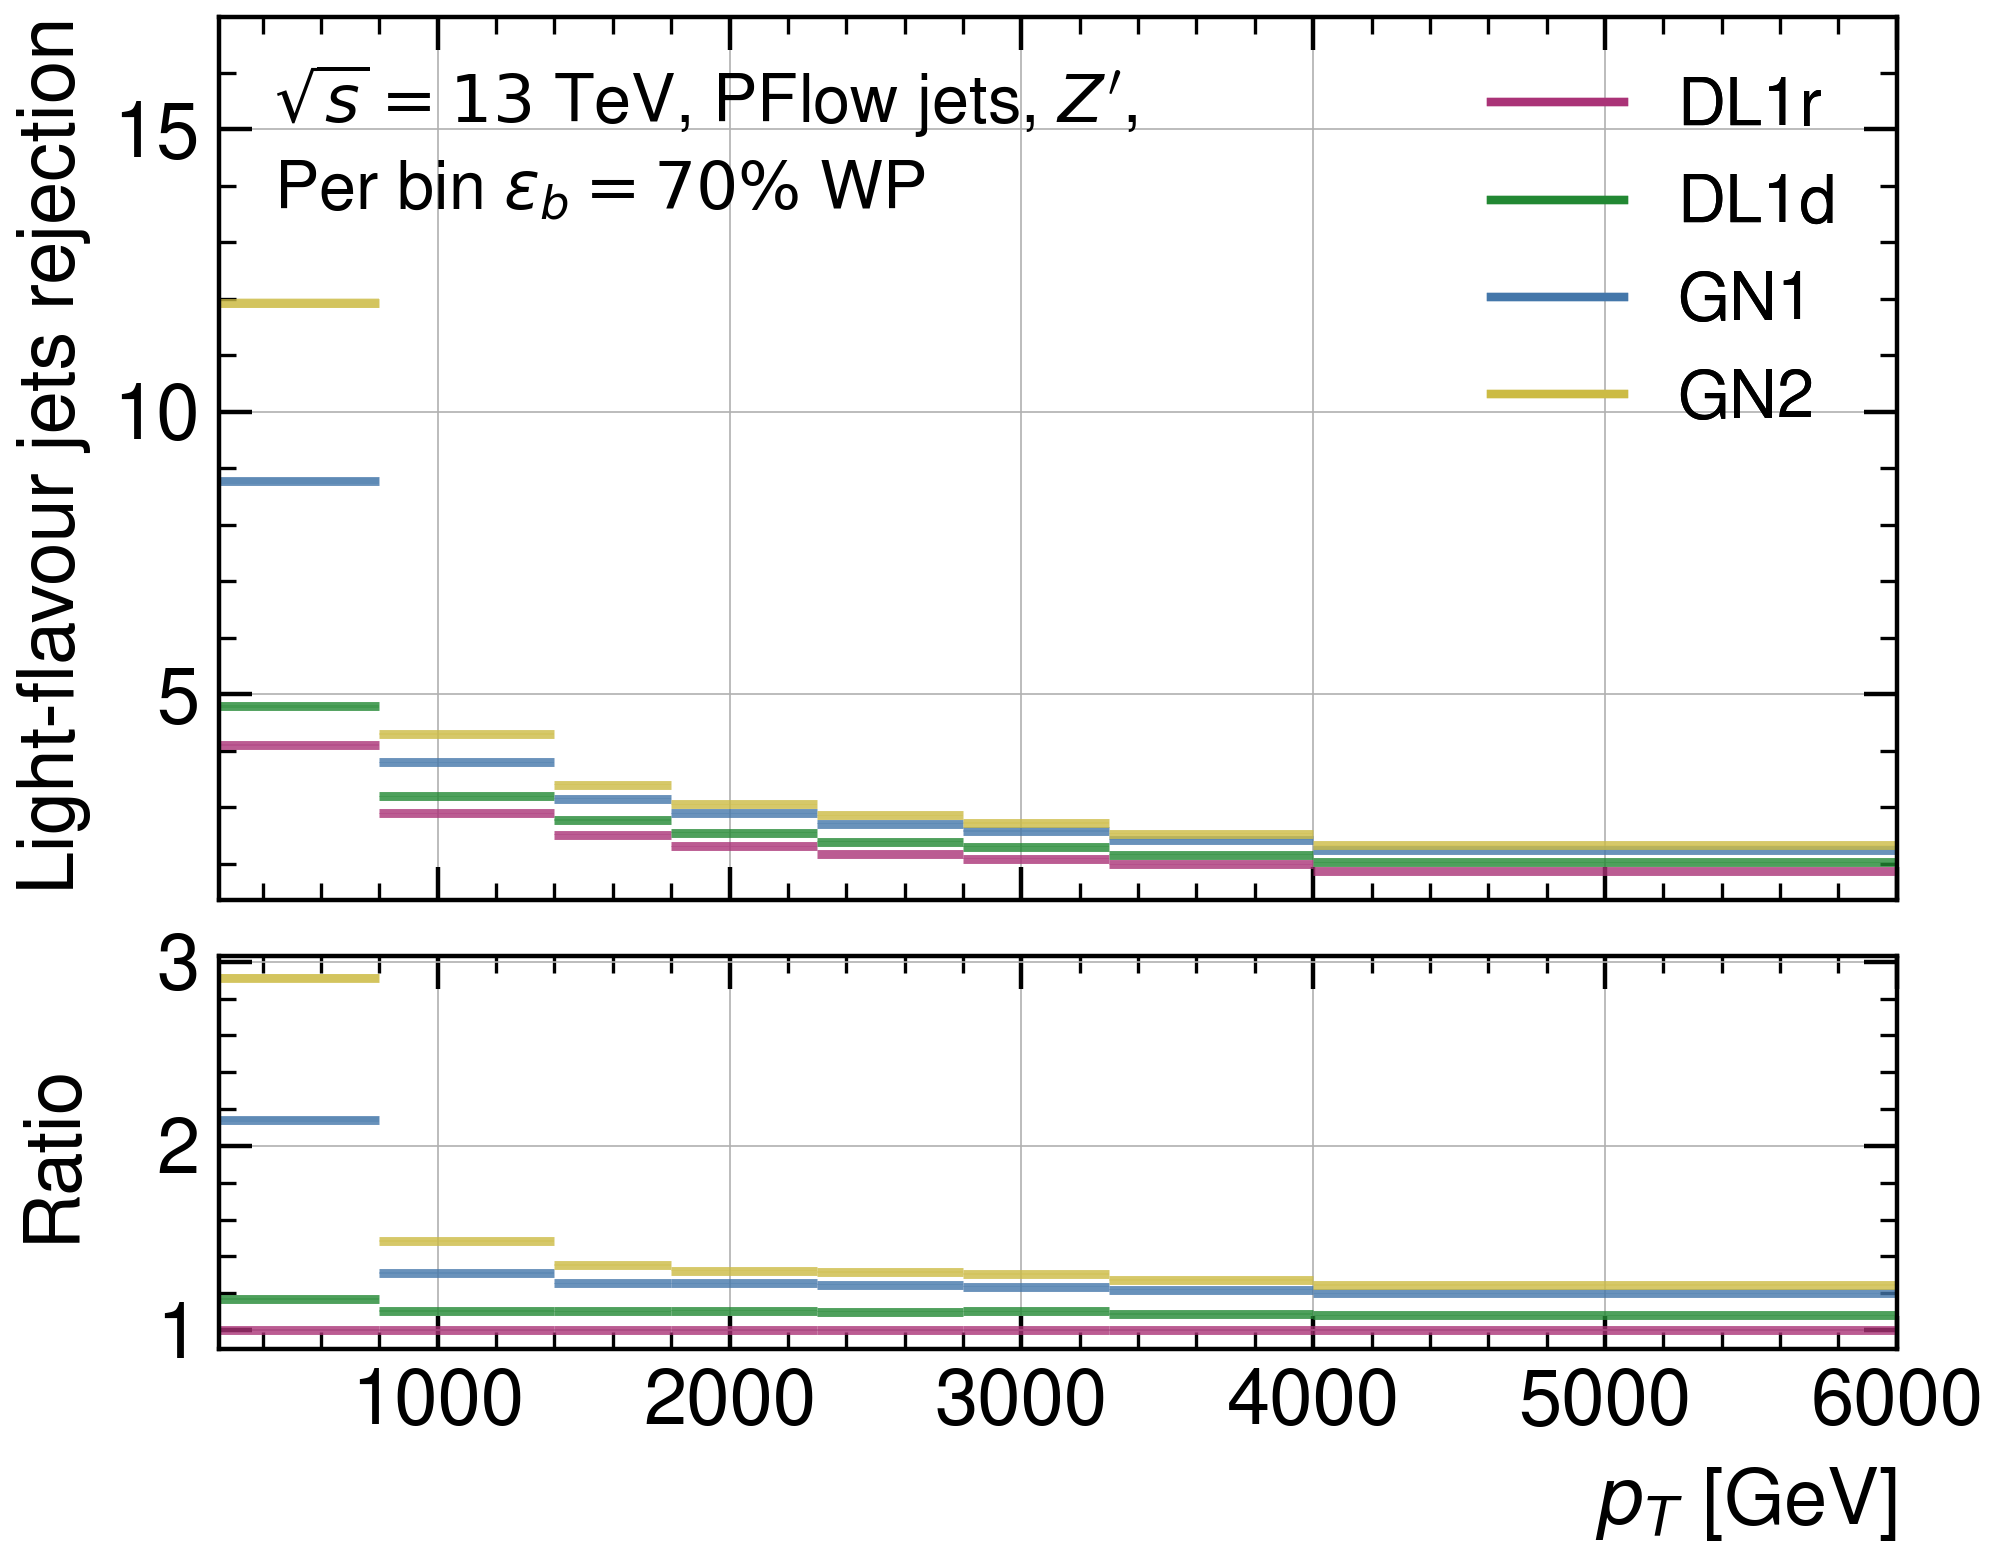
\includegraphics[width=0.48\textwidth]{Images/FTAG/GN/GN2/pt_plots/pt_zp_flat_c_rej.png}
  \caption{Comparing the different models $c$-rejection as a function of jet $p_T$ for the $b$-tagging 70\% working point per bin on the $t\bar{t}$ (left) and the 30\% working point per bin on $Z'$ (right). The flavour fraction is set at $f^b_c = 0.018$ for DL1r and DL1d, 0.05 for GN1, and 0.1 for GN2.}
  \label{fig:GNxptb_crejflat}
\end{figure} 

% Rej light -flat  btagging
\begin{figure}[h!]
  \centering
  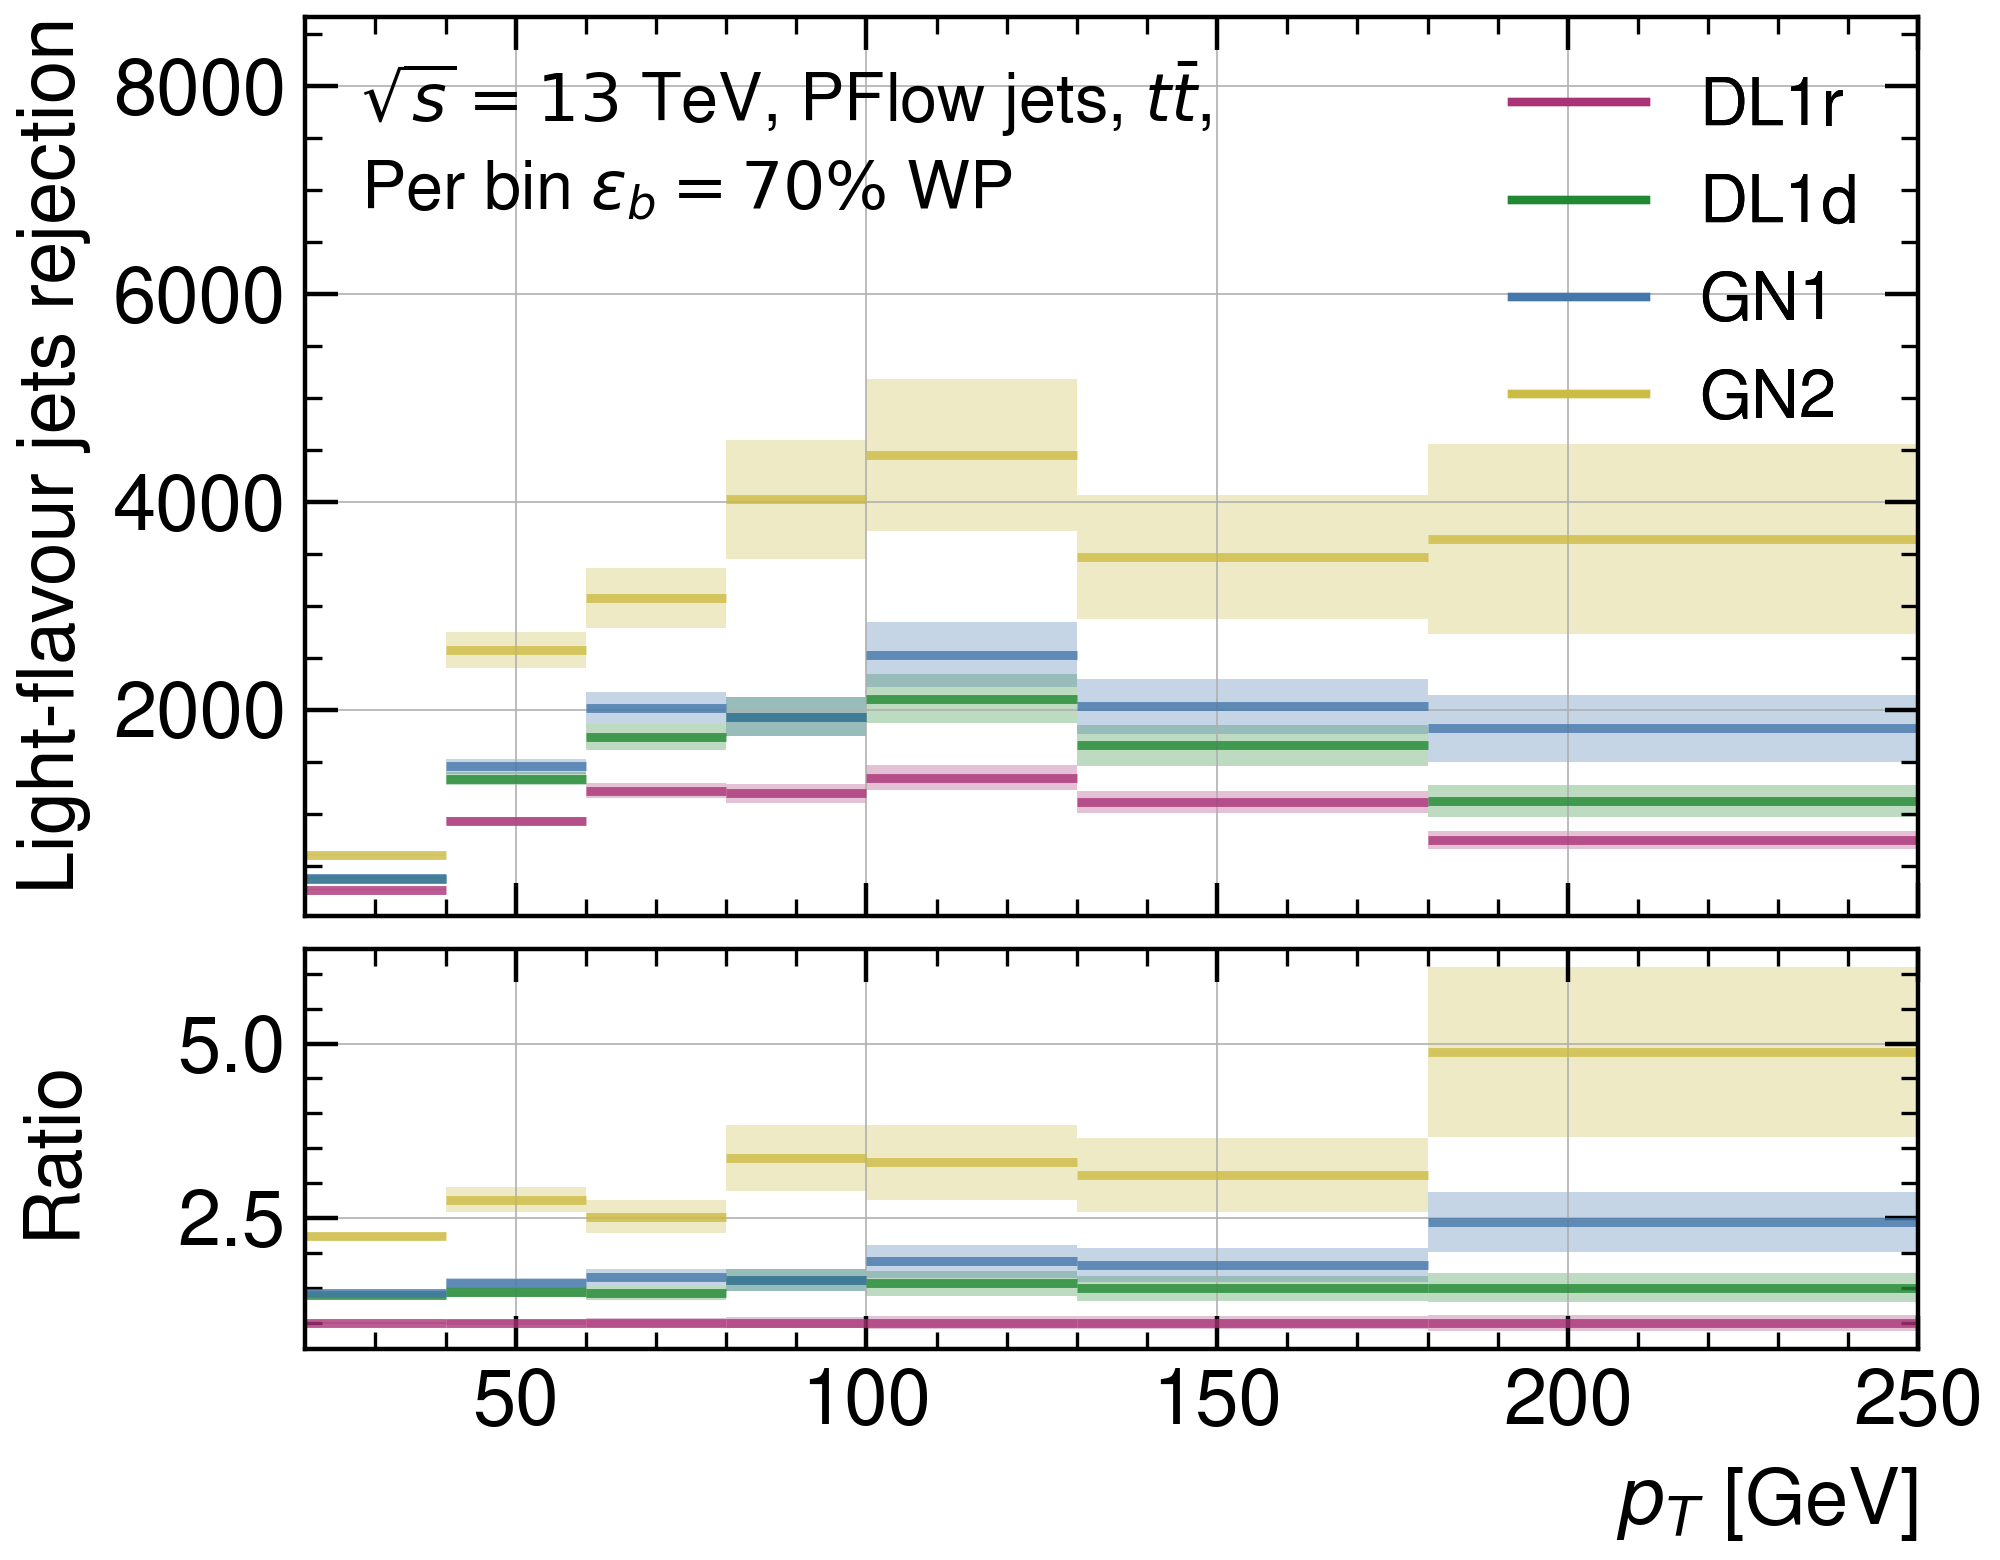
\includegraphics[width=0.48\textwidth]{Images/FTAG/GN/GN2/pt_plots/pt_ttbar_flat_light_rej.png}
  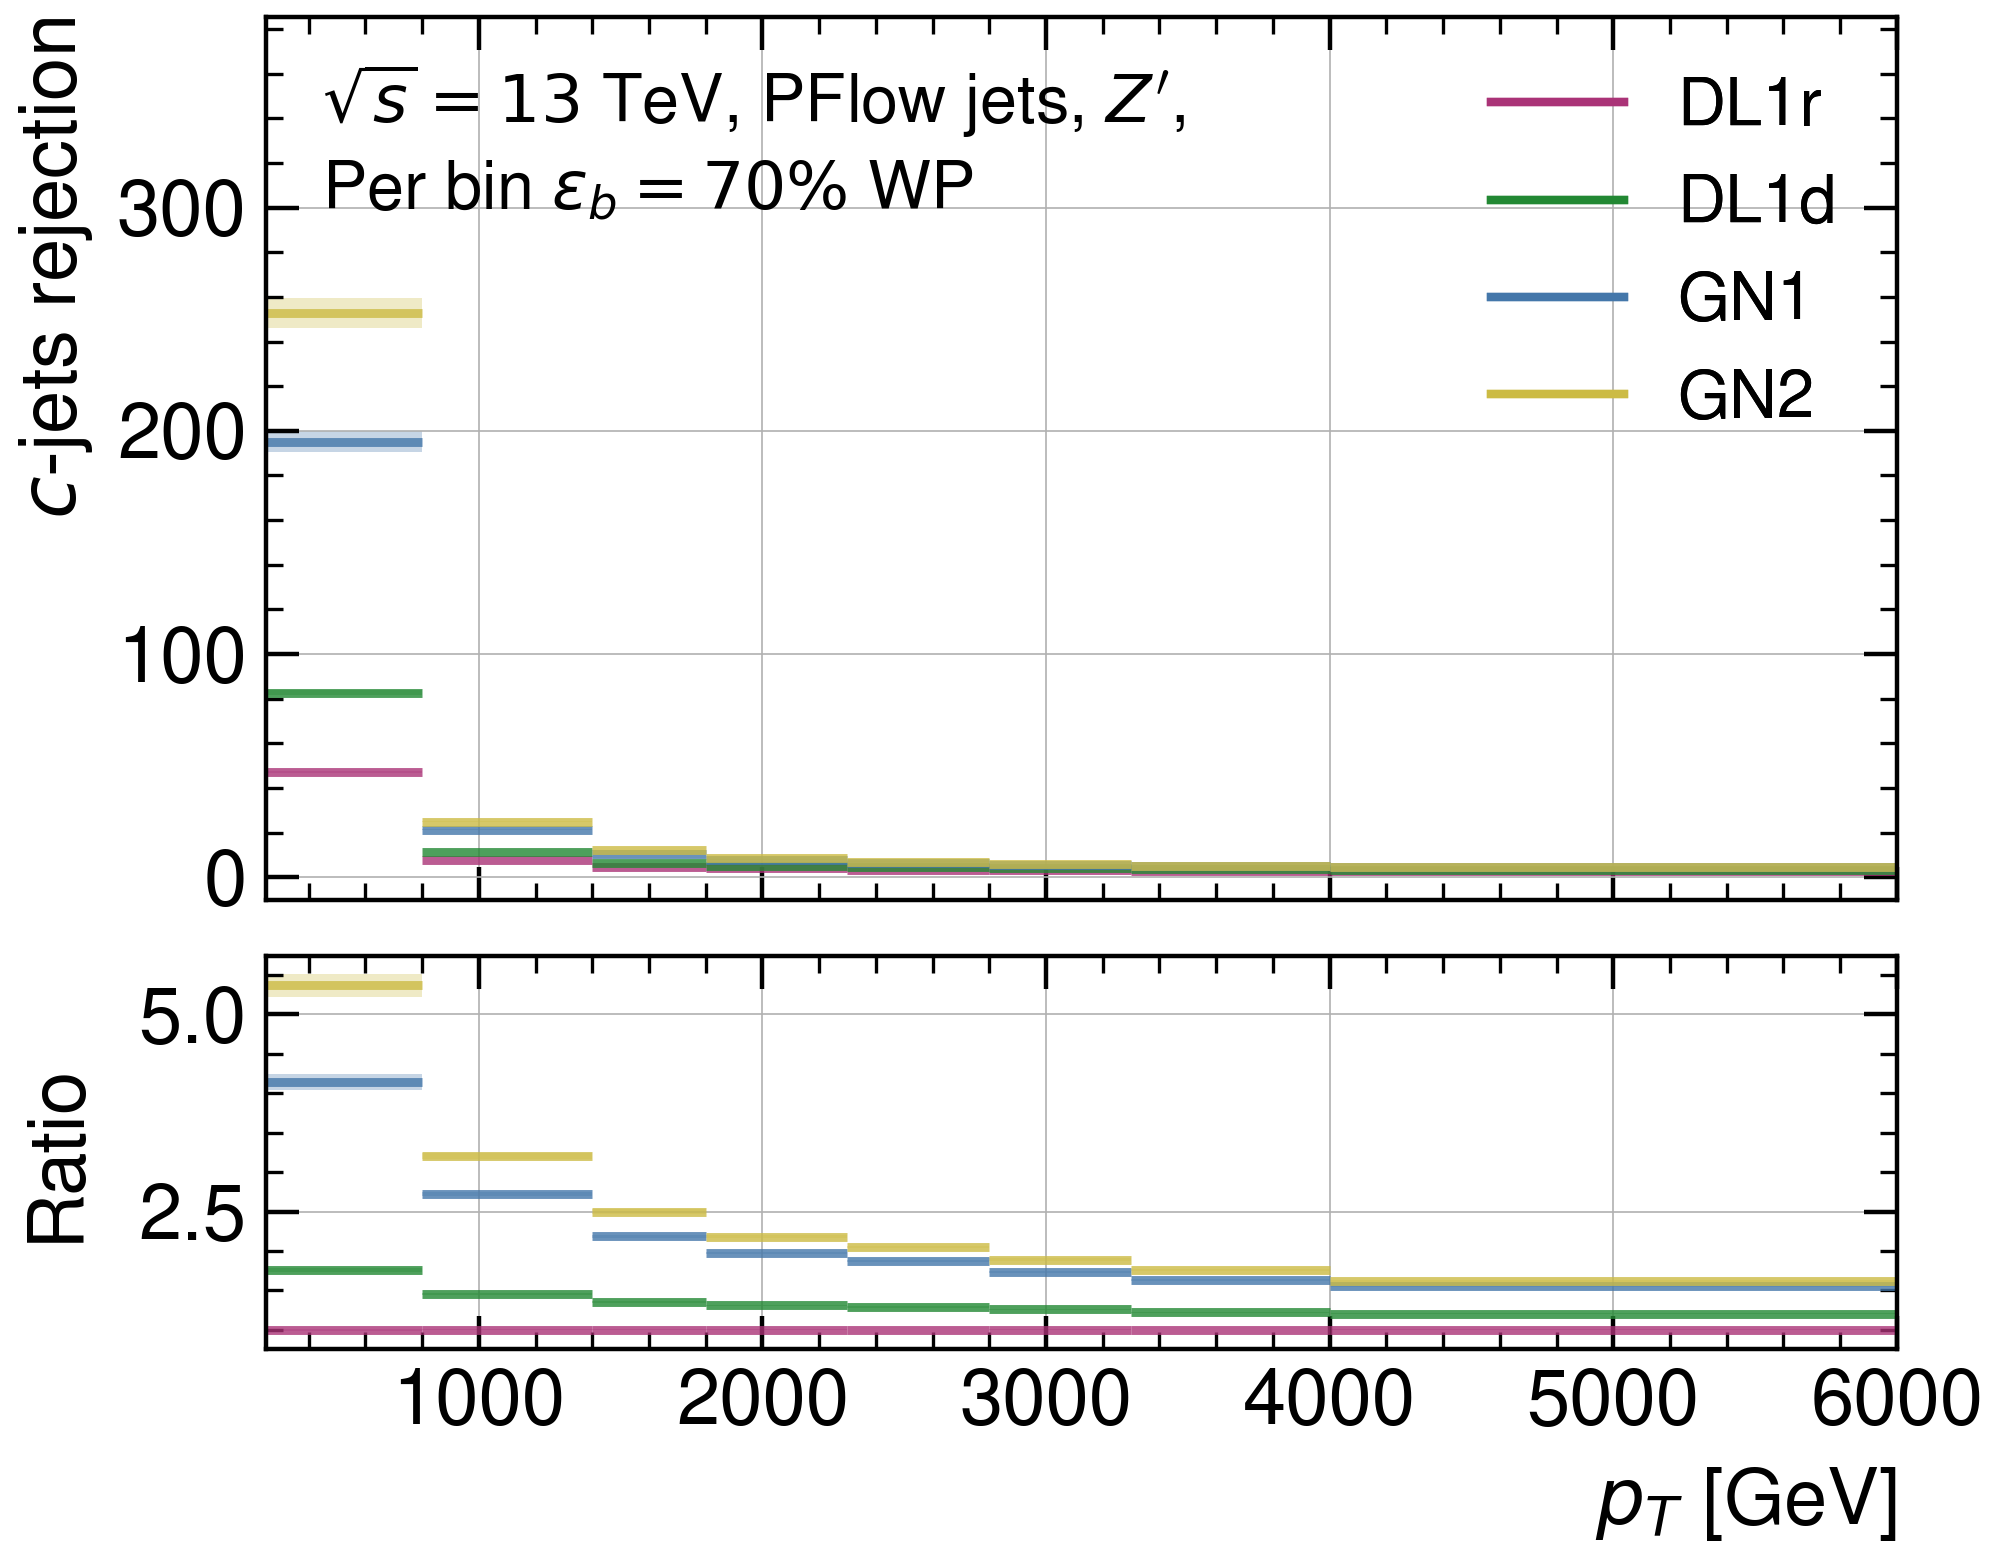
\includegraphics[width=0.48\textwidth]{Images/FTAG/GN/GN2/pt_plots/pt_zp_flat_light_rej.png}
  \caption{Comparing the different models light-rejection as a function of jet $p_T$ for the $b$-tagging 70\% working point per bin on the $t\bar{t}$ (left) and the 30\% working point per bin on $Z'$ (right). The flavour fraction is set at $f^b_c = 0.018$ for DL1r and DL1d, 0.05 for GN1, and 0.1 for GN2.}
  \label{fig:GNxptb_urejflat}
\end{figure} 

%%%


% Rej b - flat ctagging
\begin{figure}[h!]
  \centering
  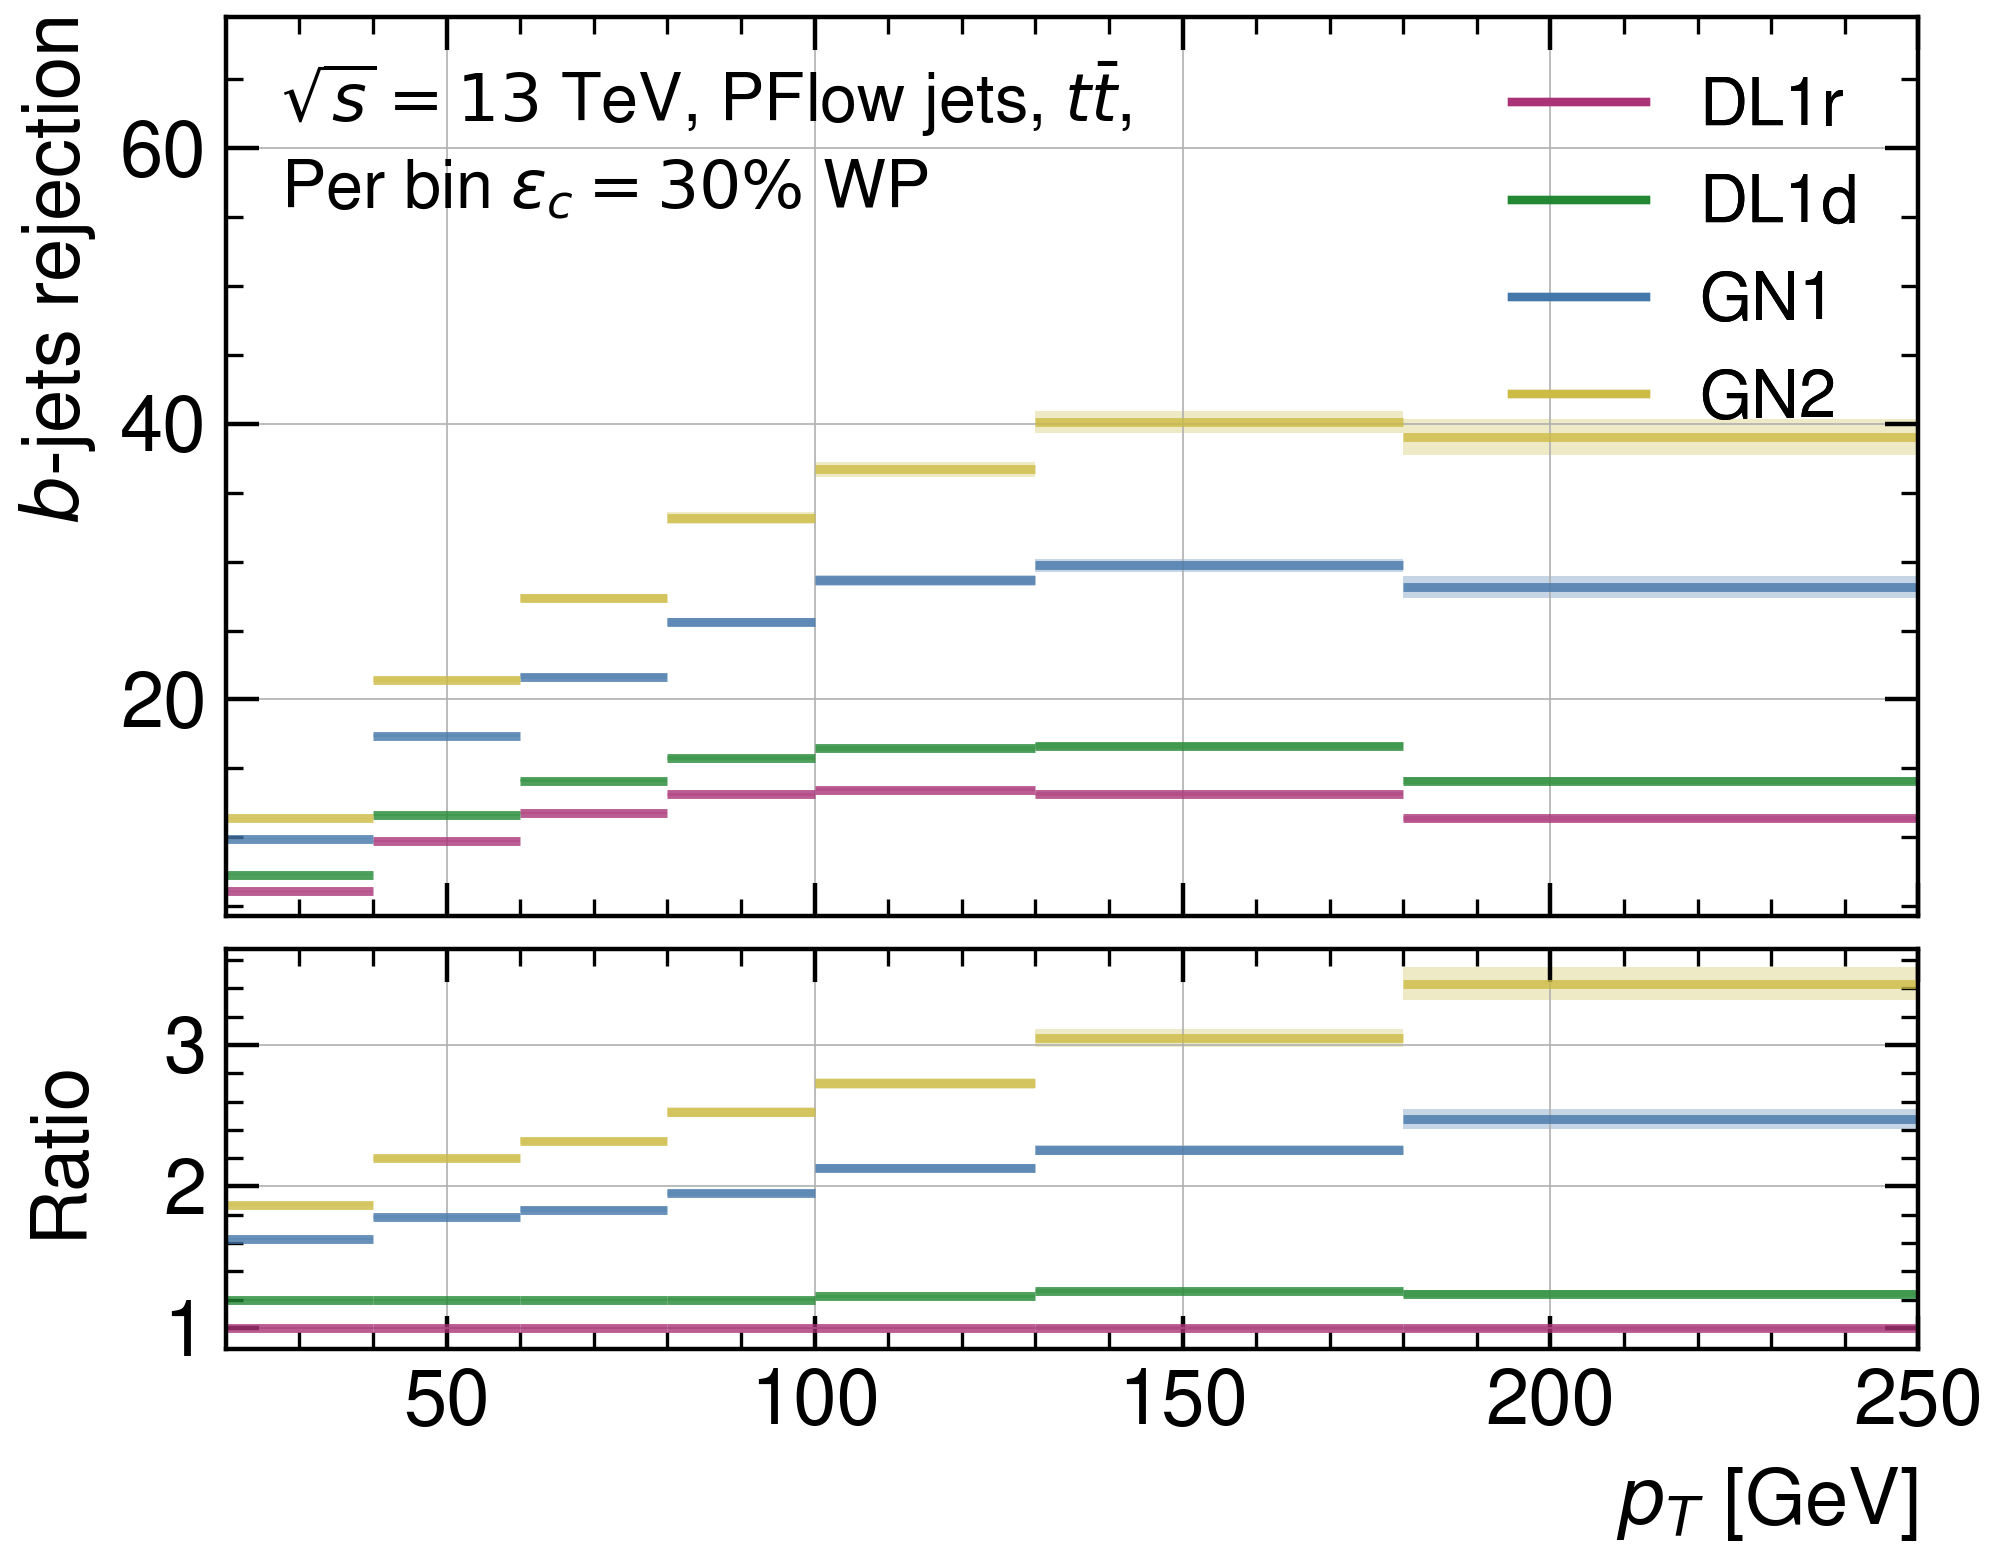
\includegraphics[width=0.48\textwidth]{Images/FTAG/GN/GN2/pt_plots/pt_ttbar_flat_b_rej_c.png}
  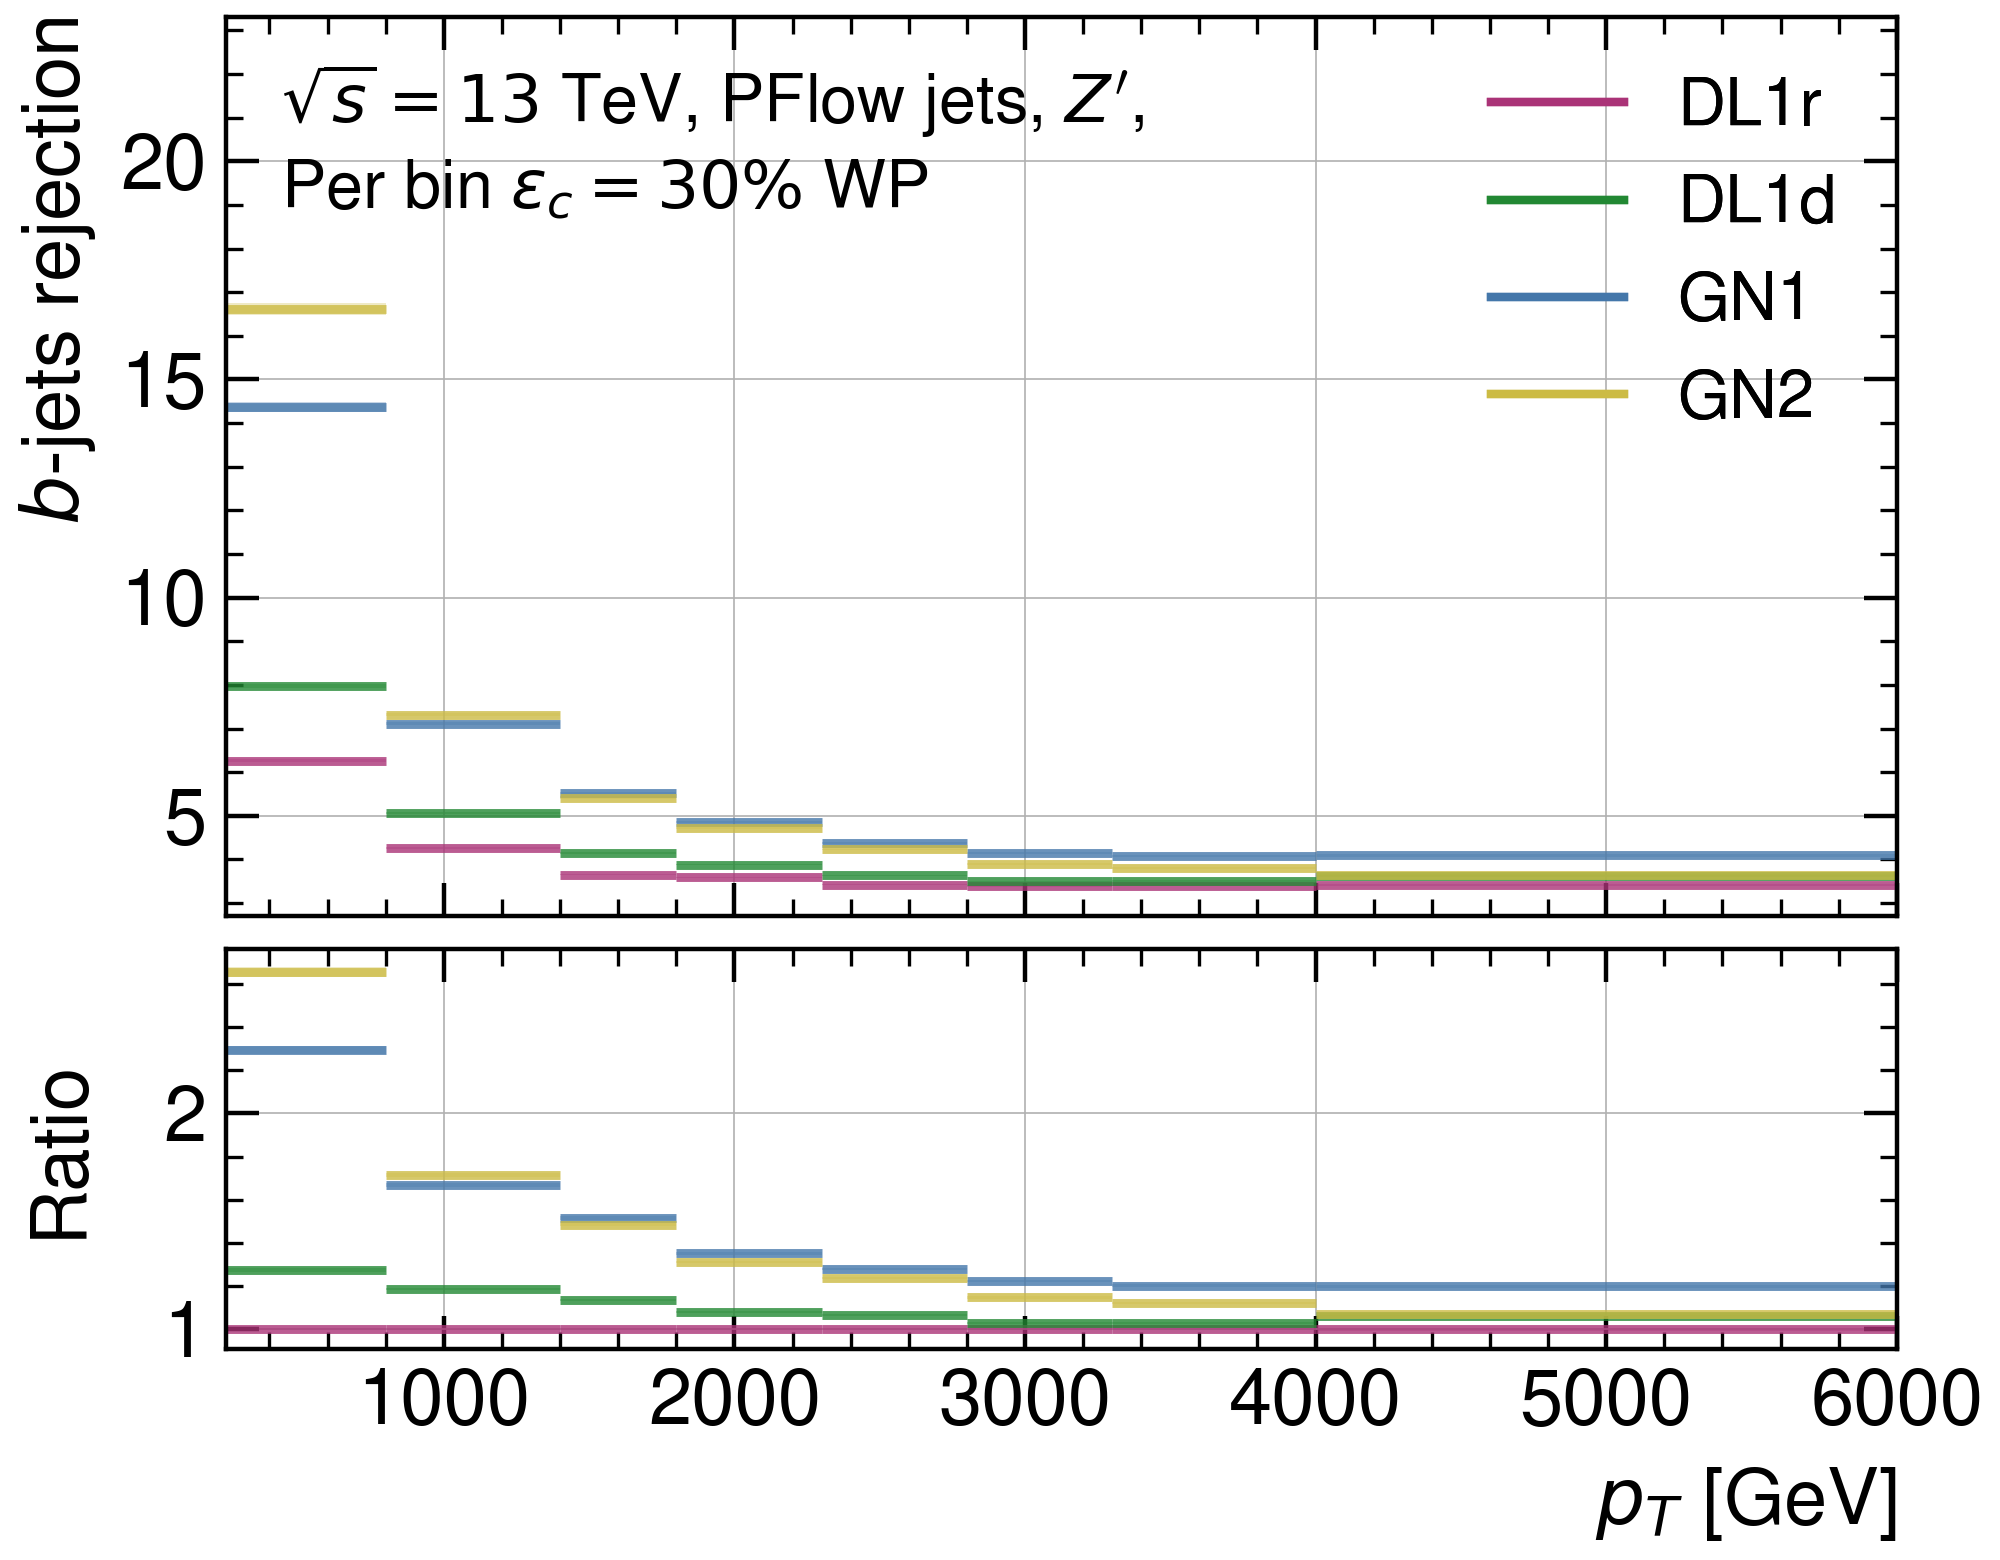
\includegraphics[width=0.48\textwidth]{Images/FTAG/GN/GN2/pt_plots/pt_zp_flat_b_rej_c.png}
  \caption{Comparing the different models $b$-rejection as a function of jet $p_T$ for the $c$-tagging 30\% working point per bin on the $t\bar{t}$ (left) and $Z'$ (right). The flavour fraction is set at $f^c_b = 0.2$ for all taggers.}
  \label{fig:GNxptc_brejflat}
\end{figure} 

% Rej light -flat  ctagging
\begin{figure}[h!]
  \centering
  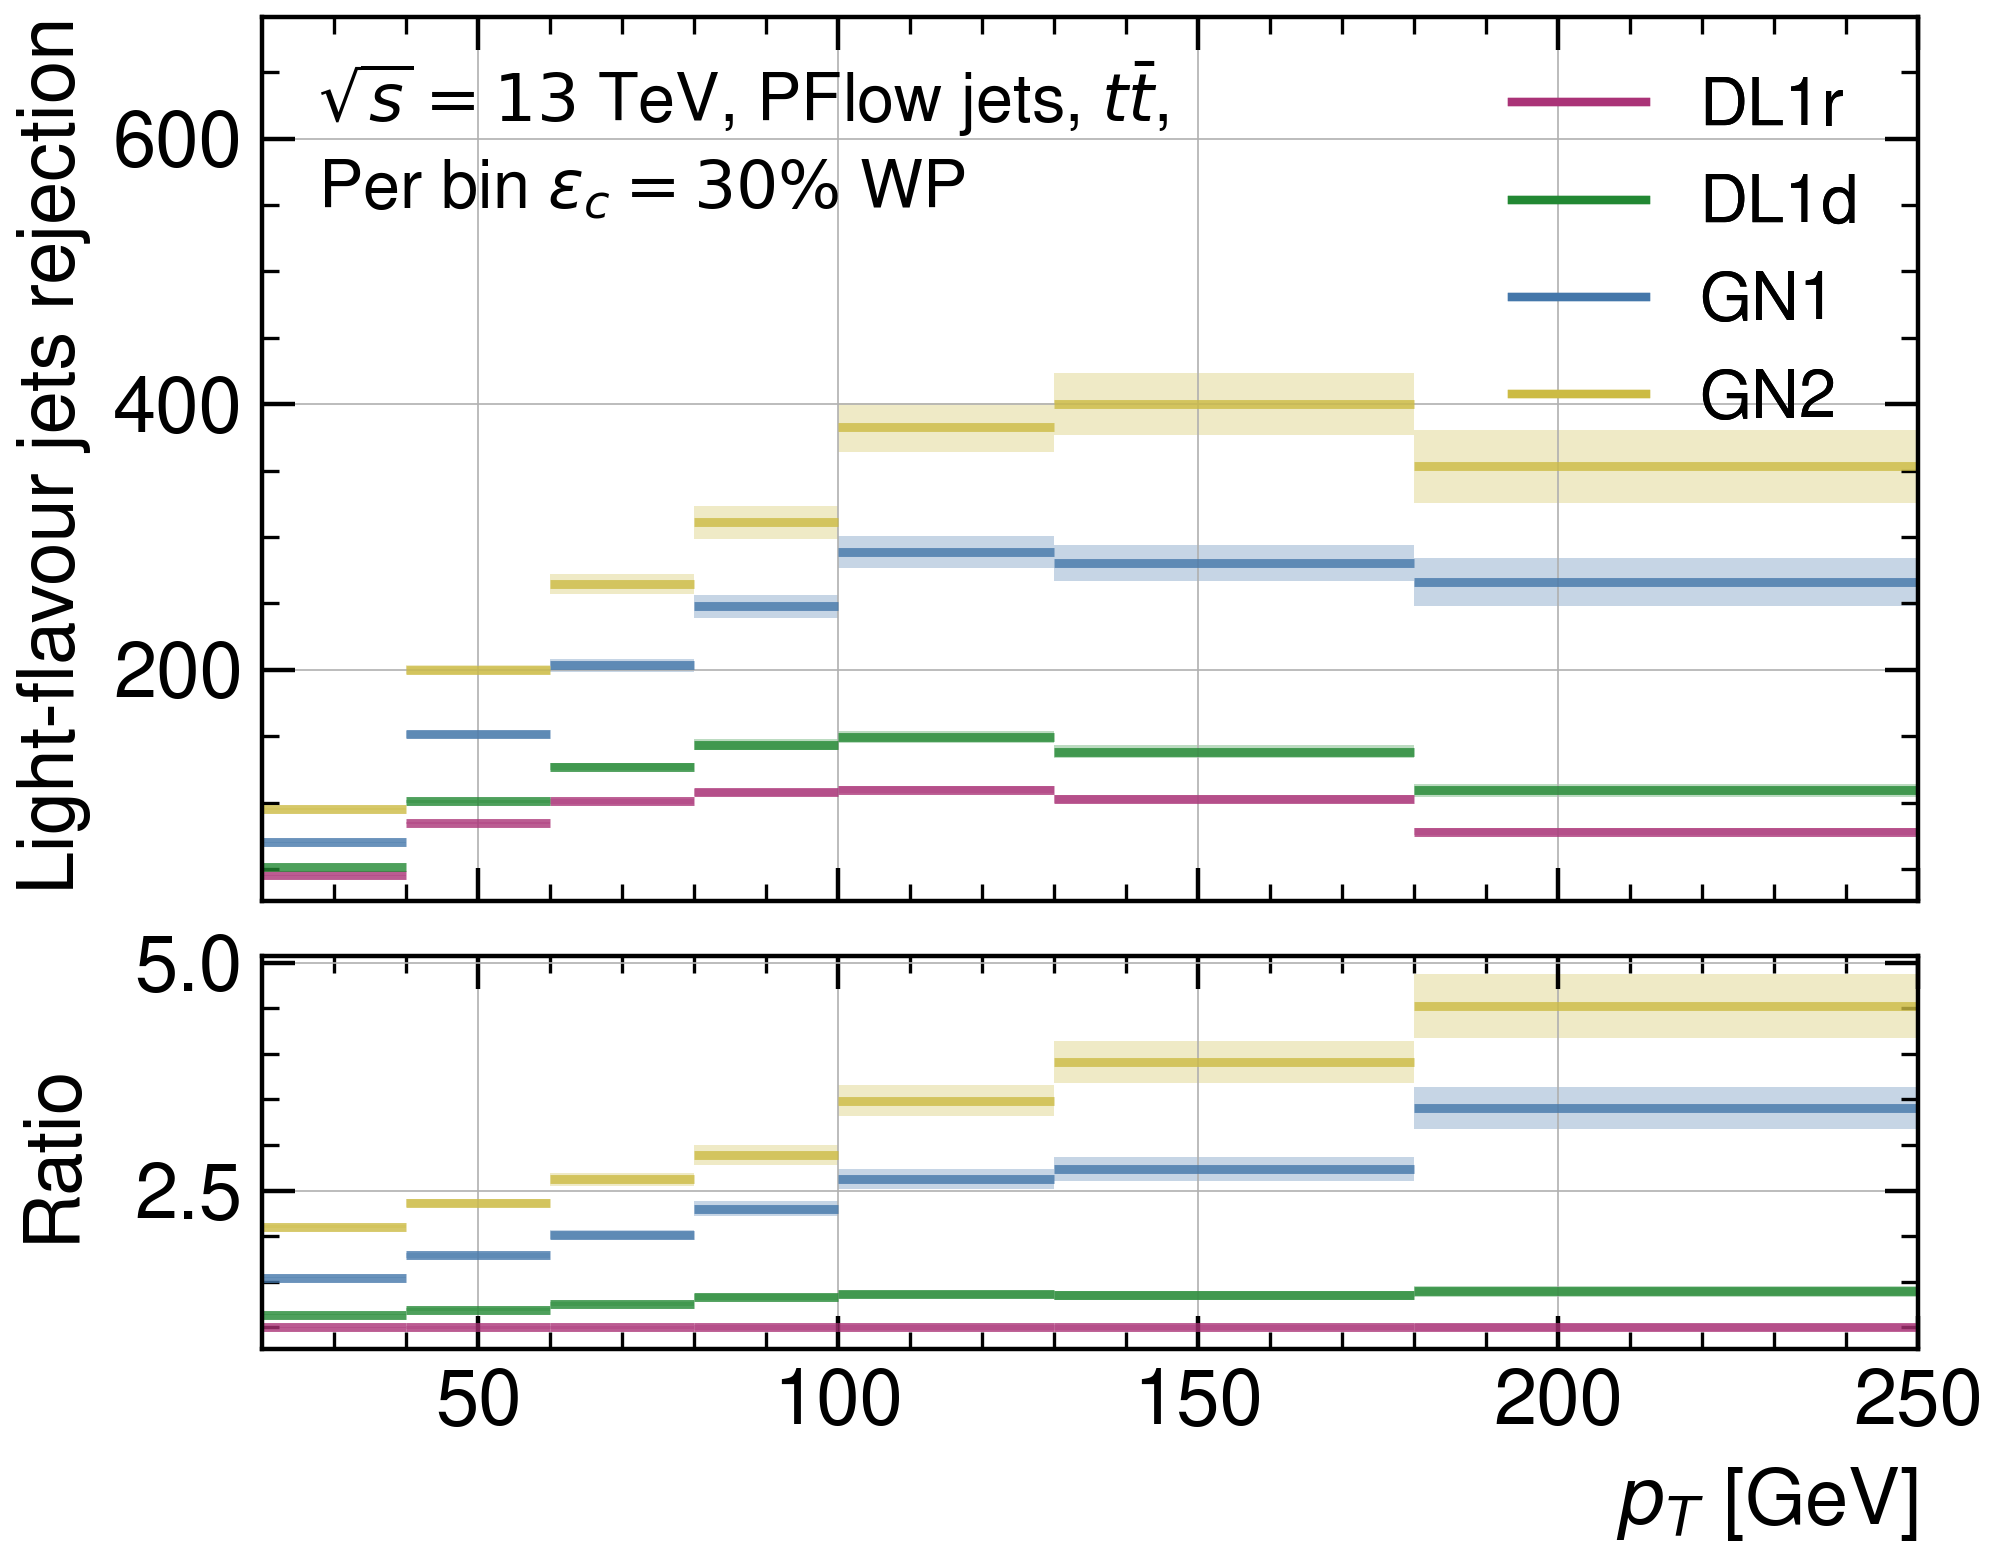
\includegraphics[width=0.48\textwidth]{Images/FTAG/GN/GN2/pt_plots/pt_ttbar_flat_light_rej_c.png}
  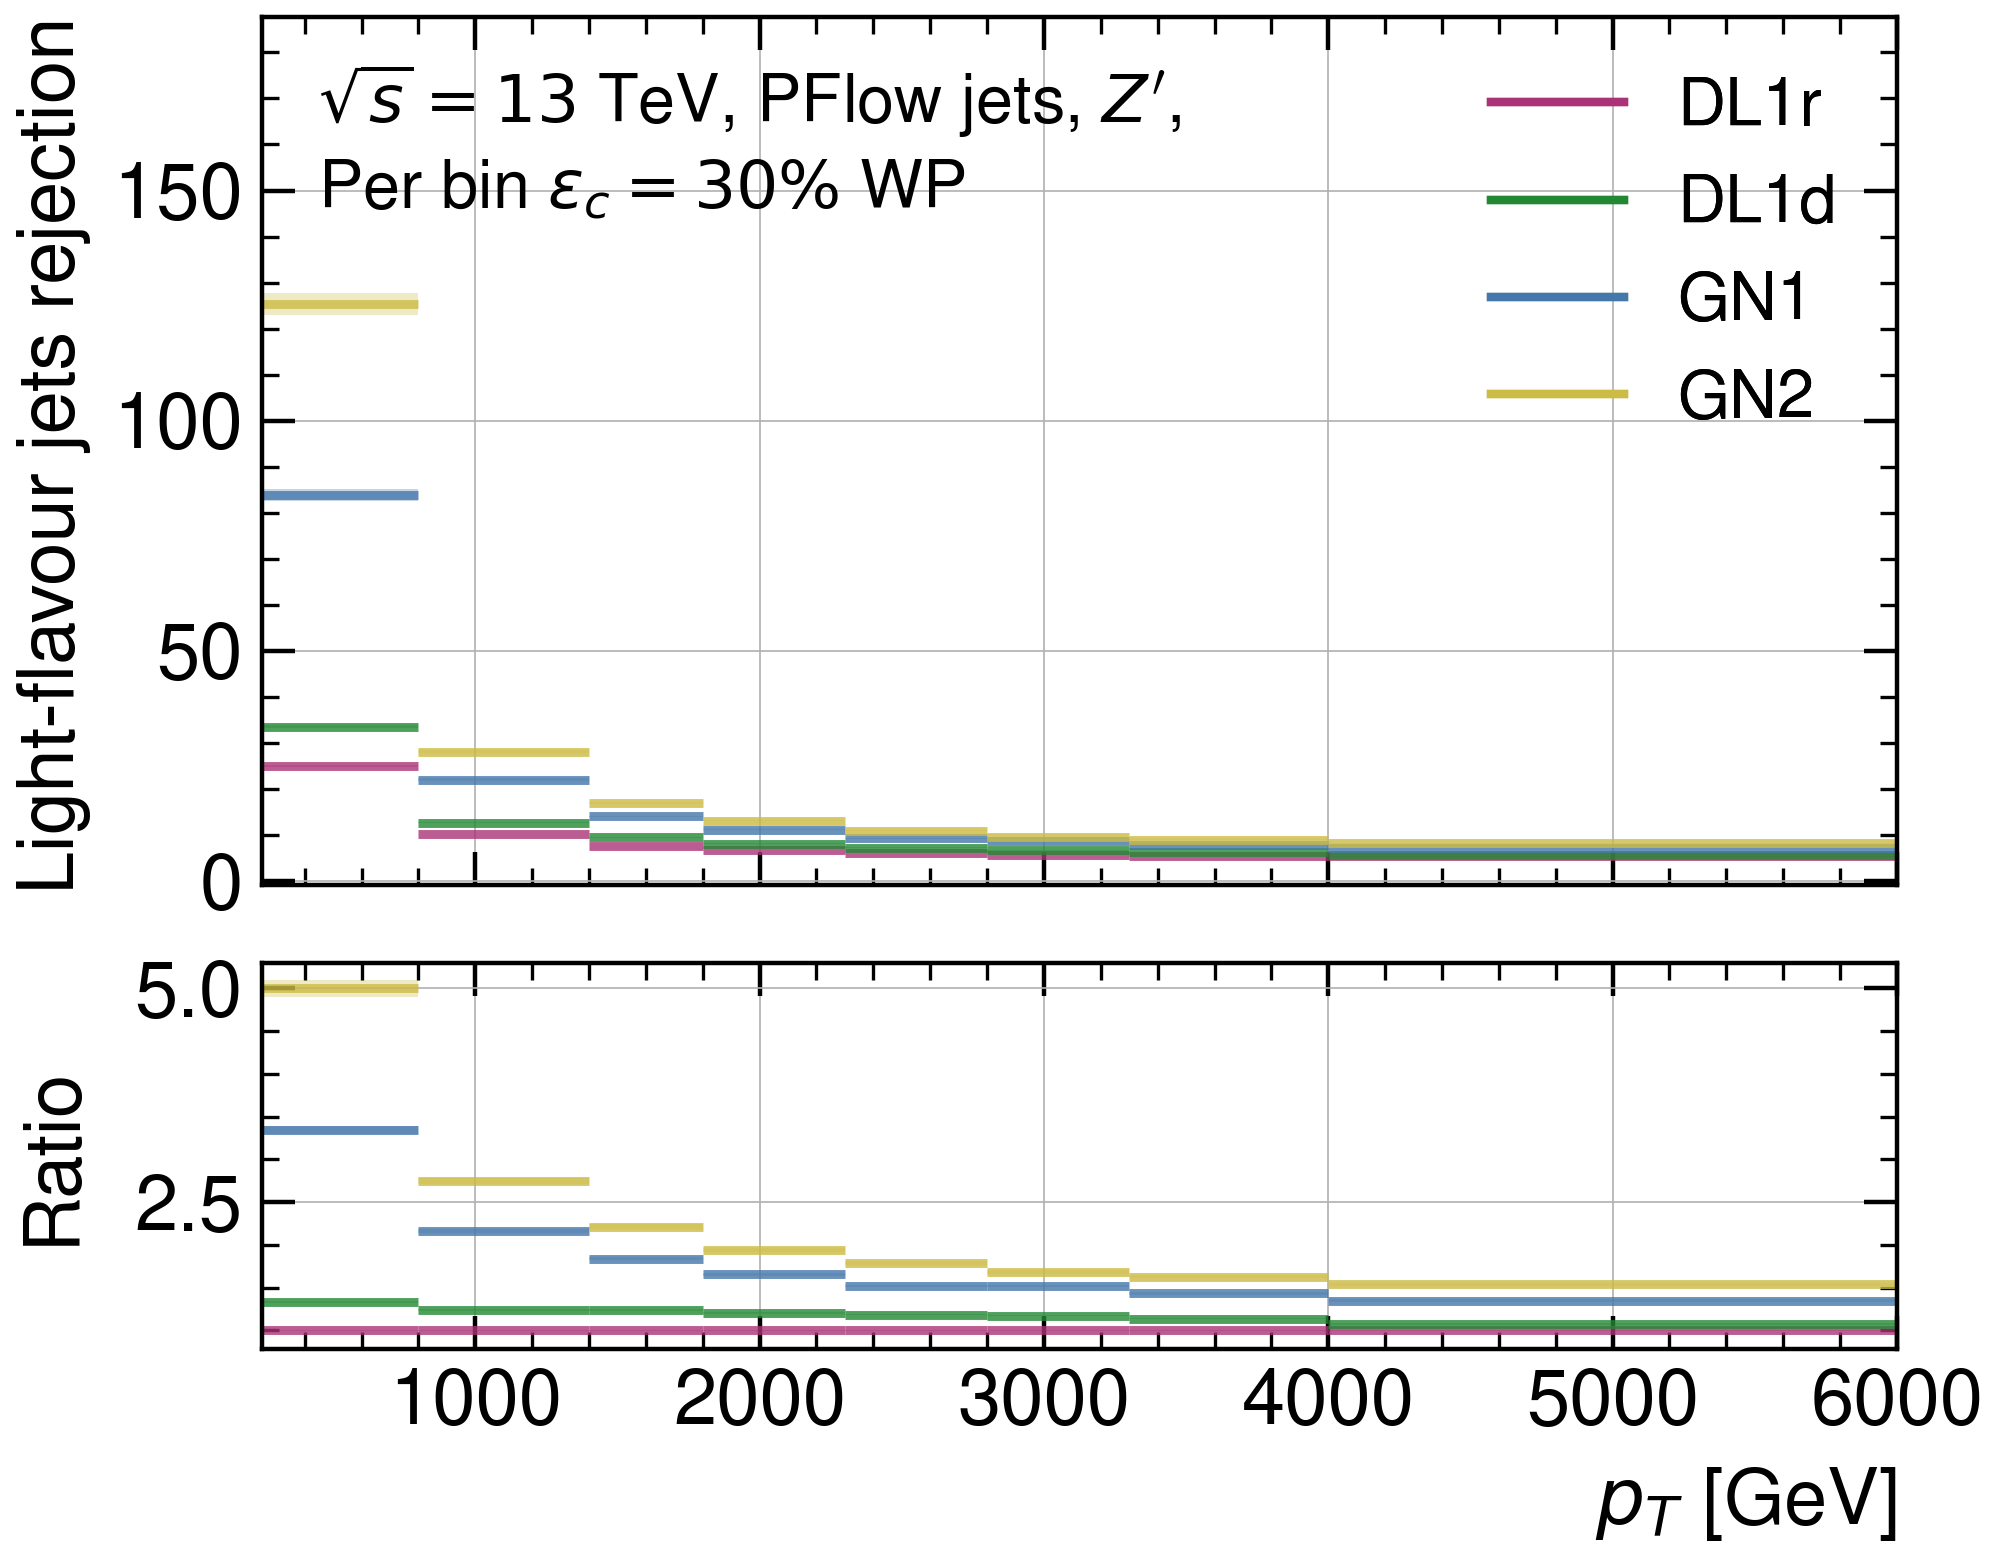
\includegraphics[width=0.48\textwidth]{Images/FTAG/GN/GN2/pt_plots/pt_zp_flat_light_rej_c.png}
  \caption{Comparing the different models light-rejection as a function of jet $p_T$ for the $c$-tagging 30\% working point per bin on the $t\bar{t}$ (left) and $Z'$ (right). The flavour fraction is set at $f^c_b = 0.2$ for all taggers.}
  \label{fig:GNxptc_urejflat}
\end{figure} 

To conclude this section, the $b$- and light-rejection at the 30\% $c$-tagging per bin working point are displayed in Figures \ref{fig:GNxptc_brejflat} and \ref{fig:GNxptc_urejflat} respectively. Clearly, most of the improvements unlocked by \gls{gn2} and \gls{gn1} is to be found in the [100, 800] GeV sweetspot of the $p_T$ spectrum. \\

These results, ableit intermediary as the developpment of the new tagger is still underway at the time of writing, are highly suggestive of the promised performance unleashed by the state-of-the-art \gls{gn2} model. Leveraging a simpler design and a more parallelisable architecture, \gls{gn2} can effectively grow to larger amount of parameters processing ever larger datasets effectively, with no significant overtraining occuring. The story of modern flavour tagging is a story of refining and ever more expressive machine learning. \gls{rnnip} and \gls{dips} required 50-60k parameters, which when used in the high-level algorithm to form \gls{dl1r} and \gls{dl1d} gives rise to models with $\sim$130k parameters. \gls{gn1} revolutionises the approach by adopting a single powerful architecture with $\sim$800k parameters. \gls{gn2} modifies this radical new design to adopt a highly efficient, regularised, and parallelisable model that easily scales the number of parameters to $\sim$1200k, being the first flavour tagger to cross the million parameters threshold. The latest design of \gls{gn2} uses 2.6M parameters, and further tests raised this number up to $\sim$70M parameters. Expert knowledge is passed to the model using supervised attention, framing the intuition as learnable tasks enforced during training. 
